% main.tex — KMITL Applied Statistics & Data Analytics Thesis (XeLaTeX)
% =====================================================================
% Compile: xelatex → biber → xelatex → xelatex
% In Overleaf: Menu → Compiler → XeLaTeX
% =====================================================================
\documentclass[12pt,a4paper,oneside]{report}

% ── Fonts (Thai + English via XeLaTeX) ─────────────────
\usepackage{fontspec}
\usepackage{polyglossia}
\setdefaultlanguage{thai}
\setotherlanguage{english}

% Auto-detect TH Sarabun New: ถ้ามีไฟล์ใน fonts/ → ใช้ Sarabun, ไม่มี → fallback ไป Norasi
\IfFontExistsTF{[./fonts/THSarabunNew.ttf]}{%
  \setmainfont[
    Path=./fonts/,
    UprightFont=THSarabunNew.ttf,
    BoldFont=THSarabunNew-Bold.ttf,
    ItalicFont=THSarabunNew-Italic.ttf,
    BoldItalicFont=THSarabunNew-BoldItalic.ttf,
    Scale=1.4,
    Ligatures=TeX
  ]{THSarabunNew}%
}{%
  \setmainfont[Ligatures=TeX,Scale=1.0]{Norasi}%
}

\setmonofont[Scale=0.9]{Latin Modern Mono}

\IfFontExistsTF{[./fonts/THSarabunNew.ttf]}{%
  \newfontfamily\thaifonttt[
    Path=./fonts/,
    UprightFont=THSarabunNew.ttf,
    BoldFont=THSarabunNew-Bold.ttf,
    Scale=1.3,
    Ligatures=TeX
  ]{THSarabunNew}%
}{%
  \newfontfamily\thaifonttt[Scale=1.0,Ligatures=TeX]{Norasi}%
}

% ── Thai line breaking (XeLaTeX) ──────────────────────
\XeTeXlinebreaklocale "th"
\XeTeXlinebreakskip = 0pt plus 1pt minus 0.1pt
\tolerance=2000
\emergencystretch=3em
\hyphenpenalty=5000
\exhyphenpenalty=5000

% ── Page geometry (KMITL) ──────────────────────────────
\usepackage[a4paper,top=3.5cm,bottom=2.5cm,left=3.5cm,right=2.5cm]{geometry}
\usepackage{setspace}
\onehalfspacing

% ── Math / tables / graphics ─────────────────────────
\usepackage{amsmath,amssymb,amsthm}
\usepackage{tabularx}
\usepackage{booktabs}
\usepackage{longtable}
\usepackage{arydshln}
\usepackage{array}
\usepackage{multirow}
\usepackage{graphicx}
\usepackage{xcolor}
\usepackage{caption}
\usepackage{subcaption}
\usepackage{enumitem}
\usepackage{listings}
\usepackage{float}
\usepackage{url}
\usepackage{tikz}
\usetikzlibrary{shapes.geometric,shapes.misc,arrows.meta,positioning,fit,backgrounds,calc}
\usepackage{pgfplots}
\pgfplotsset{compat=1.18}
\usepackage{hyperref}
\hypersetup{colorlinks=true, linkcolor=black, citecolor=blue, urlcolor=blue}

% ── Bibliography ──────────────────────────────────────
\usepackage[backend=biber,style=numeric,sorting=nyt,language=english]{biblatex}
\addbibresource{references.bib}

% ── Code listings ─────────────────────────────────────
\definecolor{codebg}{rgb}{0.96,0.96,0.96}
\definecolor{codekey}{rgb}{0.0,0.4,0.7}
\definecolor{codecom}{rgb}{0.4,0.55,0.4}
\definecolor{codestr}{rgb}{0.7,0.2,0.2}
\lstset{
  backgroundcolor=\color{codebg},
  basicstyle=\ttfamily\footnotesize,
  keywordstyle=\color{codekey}\bfseries,
  commentstyle=\color{codecom}\itshape,
  stringstyle=\color{codestr},
  numbers=left, numberstyle=\tiny, frame=single,
  breaklines=true, captionpos=b, tabsize=2,
  showstringspaces=false,
  inputencoding=utf8, extendedchars=true
}
\lstdefinelanguage{yaml}{
  keywords={true,false,null},
  sensitive=true,
  comment=[l]{\#},
  morestring=[b]',
  morestring=[b]"
}

% ── Captions in Thai ──────────────────────────────────
\addto\captionsthai{%
  \renewcommand{\contentsname}{สารบัญ}%
  \renewcommand{\listfigurename}{สารบัญรูป}%
  \renewcommand{\listtablename}{สารบัญตาราง}%
  \renewcommand{\bibname}{เอกสารอ้างอิง}%
  \renewcommand{\appendixname}{ภาคผนวก}%
  \renewcommand{\chaptername}{บทที่}%
  \renewcommand{\figurename}{ภาพที่}%
  \renewcommand{\tablename}{ตารางที่}%
  \renewcommand{\abstractname}{บทคัดย่อ}%
}

% ── Thesis metadata ────────────────────────────────────
\newcommand{\thesistitleTH}{การศึกษาเชิงเปรียบเทียบของแบบจำลองทรานส์ฟอร์เมอร์ภาษาไทยสำหรับพยากรณ์ความไวรัลของวิดีโอ YouTube: WangchanBERTa, PhayaThaiBERT และ XLM-RoBERTa-large}
\newcommand{\thesistitleEN}{A Comparative Study of Thai Transformer Language Models for YouTube Video Virality Prediction: WangchanBERTa, PhayaThaiBERT, and XLM-RoBERTa-large}
\newcommand{\authorone}{นายตรัยภูรินท์ สืบสุวรรณสาร}
\newcommand{\authortwo}{นายธีรนนท์ ไชยลังกา}
\newcommand{\authorthree}{นายภาณุเดช ภู่โทสนธิ์}
\newcommand{\authoroneEN}{Mr.\ Traipoohrin Suebuswansarn}
\newcommand{\authortwoEN}{Mr.\ Teeranon Chailangka}
\newcommand{\authorthreeEN}{Mr.\ Phanudech Phuthoson}
\newcommand{\studentidone}{65050330}
\newcommand{\studentidtwo}{65050417}
\newcommand{\studentidthree}{65050685}
\newcommand{\advisor}{ผศ.\ ดร.\ พรพิมล\ ชัยวุฒิศักดิ์}
\newcommand{\advisorEN}{Asst.\ Prof.\ Dr.\ Pornpimol Chaiwuttisak}
\newcommand{\academicyear}{2568}
\newcommand{\academicyearEN}{2025}
\newcommand{\department}{ภาควิชาสถิติประยุกต์และการวิเคราะห์ข้อมูล}
\newcommand{\school}{คณะวิทยาศาสตร์}
\newcommand{\university}{สถาบันเทคโนโลยีพระจอมเกล้าเจ้าคุณทหารลาดกระบัง}
\newcommand{\universityEN}{King Mongkut's Institute of Technology Ladkrabang}

\begin{document}

% frontmatter/cover.tex — หน้าปกปัญหาพิเศษ KMITL
\thispagestyle{empty}
\begin{center}
  \vspace*{0.1cm}

  
\includegraphics[width=3.2cm]{figures/kmitl_logo.png}\\[0.4cm]

  % {\Large\bfseries ปัญหาพิเศษ}

  % \vspace{1cm}
  % {\large เรื่อง}

  \vspace{0.8cm}
  \begin{minipage}{0.92\textwidth}
    \begin{center}
      {\large\bfseries\thesistitleTH\par}
    \end{center}
  \end{minipage}

  \vspace{1.2cm}
  \begin{minipage}{0.92\textwidth}
    \begin{center}
      {\large\bfseries\thesistitleEN\par}
    \end{center}
  \end{minipage}

  \vspace{1.6cm}
  จัดทำโดย

  \vspace{0.4cm}
  {\large \authorone\quad รหัสนักศึกษา\ \studentidone}\\[2pt]
  {\large \authortwo\quad รหัสนักศึกษา\ \studentidtwo}\\[2pt]
  {\large \authorthree\quad รหัสนักศึกษา\ \studentidthree}

  \vspace{1.2cm}
  อาจารย์ที่ปรึกษา

  \vspace{0.3cm}
  {\large \advisor}

  \vspace{1.4cm}
  ปัญหาพิเศษนี้เป็นส่วนหนึ่งของการศึกษาตามหลักสูตร

  ปริญญาวิทยาศาสตรบัณฑิต (สถิติประยุกต์และการวิเคราะห์ข้อมูล)

  \department\ \school

  \university

  ปีการศึกษา \academicyear
\end{center}
\newpage

% frontmatter/approval.tex — หน้าอนุมัติ
\thispagestyle{empty}

\noindent\textbf{หัวข้อปัญหาพิเศษ}\hfill\thesistitleTH

\vspace{0.4cm}
\noindent\textbf{}\hfill\thesistitleEN

\vspace{0.6cm}
\noindent\textbf{ชื่อนักศึกษา}\hfill\authorone\quad รหัสนักศึกษา \studentidone\\
\hspace*{0pt}\hfill \authortwo\quad รหัสนักศึกษา \studentidtwo\\
\hspace*{0pt}\hfill \authorthree\quad รหัสนักศึกษา \studentidthree

\vspace{0.4cm}
\noindent\textbf{ปริญญา}\hfill วิทยาศาสตรบัณฑิต (สถิติประยุกต์)

\noindent\textbf{ภาควิชา}\hfill สถิติประยุกต์และการวิเคราะห์ข้อมูล

\noindent\textbf{ปีการศึกษา}\hfill \academicyear

\noindent\textbf{อาจารย์ที่ปรึกษา}\hfill \advisor

\vspace{1.2cm}
\noindent \school\ \university\ (สจล.) อนุมัติให้
ปัญหาพิเศษนี้เป็นส่วนหนึ่งของการศึกษาตามหลักสูตรปริญญาวิทยาศาสตรบัณฑิต
(สถิติประยุกต์และการวิเคราะห์ข้อมูล) ประจำปีการศึกษา \academicyear.

\vspace{1.5cm}
\begin{center}
\textbf{คณะกรรมการสอบ}
\end{center}

\vspace{0.6cm}
\noindent\hspace{2cm}\rule{8cm}{0.4pt}\hspace{0.5cm}ประธานกรรมการ\\
\hspace*{2cm}(\,ดร.\ อัครชัย อินทนิล\,)

\vspace{1cm}
\noindent\hspace{2cm}\rule{8cm}{0.4pt}\hspace{0.5cm}กรรมการ\\
\hspace*{2cm}(\,อ.\ สุจิตรา สุคนธมัต\,)

\vspace{1cm}
\noindent\hspace{2cm}\rule{8cm}{0.4pt}\hspace{0.5cm}อาจารย์ที่ปรึกษา\\
\hspace*{2cm}(\,\advisor\,)

\newpage

% frontmatter/abstract-th.tex — บทคัดย่อภาษาไทย
\chapter*{บทคัดย่อ}
\addcontentsline{toc}{chapter}{บทคัดย่อภาษาไทย}

\noindent\textbf{หัวข้อปัญหาพิเศษ:}\ \thesistitleTH\\
\textbf{โดย:}\ \authorone, \authortwo, \authorthree\\
\textbf{อาจารย์ที่ปรึกษา:}\ \advisor\\
\textbf{ปีการศึกษา:}\ \academicyear

\vspace{0.6cm}

แพลตฟอร์มวิดีโอ YouTube มีผู้ใช้งานต่อเดือนมากกว่า 2.5 พันล้านคน และเป็นช่องทางการตลาด
ที่สำคัญของผู้สร้างเนื้อหาภาษาไทย การพยากรณ์ \emph{ความไวรัล} (virality) ของวิดีโอตั้งแต่
ก่อนเผยแพร่ จึงมีคุณค่าในเชิงพาณิชย์และเชิงวิชาการ งานวิจัยนี้กำหนดปัญหาเป็นการจำแนก
ประเภททวิภาคของวิดีโอภาษาไทยว่าจะเป็นไวรัลหรือไม่ โดยใช้ \emph{ดัชนีความไวรัลภายในช่อง}
(Per-channel Virality Index, $\mathit{VI}$) ซึ่งสร้างจากผลรวมแบบถ่วงน้ำหนักของอัตรา
ส่วนการมีส่วนร่วม (engagement rate) อัตราส่วนการกดถูกใจ และอัตราส่วนความคิดเห็น
หลังการแปลงด้วยลอการิทึมและ z-score ภายในช่องเจ้าของ ป้ายกำกับเชิงบวกถูกกำหนดเป็น
เดไซล์บนสุด (top-decile) ของแต่ละช่องเพื่อหลีกเลี่ยงไม่ให้ขนาดช่องเป็นปัจจัยรบกวน

ชุดข้อมูลประกอบด้วยวิดีโอจำนวน 23{,}431 รายการจาก 82 ช่องที่จัดเก็บผ่าน YouTube Data
API v3 มีอัตราส่วนคลาสบวก 10.16\% การแบ่งชุดข้อมูลใช้ \emph{แบบไวต่อเวลาผสมจัดกลุ่ม
ตามช่อง} (channel-grouped, time-aware split) โดยกำหนดให้ชุดทดสอบเป็นวิดีโอที่ตีพิมพ์
ในช่วง 15\% หลังสุดตามเวลา และทำการสุ่มลดข้อมูล (undersampling) ในอัตราส่วน 3:1
\emph{เฉพาะชุดฝึกฝนเท่านั้น} เพื่อรักษาการกระจายตัวตามธรรมชาติของชุดตรวจสอบและ
ชุดทดสอบ

งานวิจัยเปรียบเทียบแบบจำลองทรานส์ฟอร์เมอร์ภาษาไทยขนาดและสถาปัตยกรรมต่างกัน
3 แบบ ได้แก่ \textbf{WangchanBERTa} (105M, RoBERTa SentencePiece) \textbf{PhayaThaiBERT}
(278M, RoBERTa) และ \textbf{XLM-RoBERTa-large} (560M, multilingual) ทุกแบบจำลอง
ปรับจูนแบบเต็ม (full fine-tuning) บน GPU NVIDIA T4/A10G ผ่าน Hugging Face Jobs
แบบจำลองพื้นฐาน (Logistic Regression, LightGBM, XGBoost) ใช้ชุดคุณลักษณะเชิงโครงสร้าง
27 ตัว ผสมกับ TF-IDF อักขระ-N-gram และฟีเจอร์อารมณ์ (sentiment) จาก Wisesight-Sentiment
นอกจากนี้ยังพัฒนาแบบจำลอง \emph{ไฮบริด} (MLP + LightGBM head) ซึ่งใช้เวกเตอร์ฝัง
ข้อความรวมกับฟีเจอร์เชิงโครงสร้าง ปิดท้ายด้วย \emph{การประกอบแบบเรียงซ้อน} (stacking
ensemble) ที่ใช้ Logistic Regression เป็นตัวเรียนระดับเมตา (meta-learner) บนความน่าจะเป็น
ของฐาน 15 แบบจำลอง

จากการประเมินบนชุดทดสอบเดียวกัน แบบจำลองที่ดีที่สุดคือ \textbf{stacking ensemble
ที่ปรับเทียบด้วย Platt} ซึ่งให้ค่า ROC-AUC = \textbf{0.6914} โดยมีช่วงความเชื่อมั่นบูตสแตรป
95\% \textbf{[0.6625, 0.7174]}, ECE = 0.016 ซึ่งสูงกว่าแบบจำลองที่ดีที่สุดเดี่ยว
(LightGBM-Structured+TF-IDF, 0.6728) อย่างมีนัยสำคัญ ($p$ = $6.9\!\times\!10^{-53}$
จาก McNemar's test) ในระดับแบบจำลองทรานส์ฟอร์เมอร์เดี่ยว PhayaThaiBERT (0.6451)
ทำงานได้ดีที่สุด ตามด้วย WangchanBERTa (0.6402) และ XLM-RoBERTa-large (0.5450)
การทดสอบ Cochran's Q ระหว่างทรานส์ฟอร์เมอร์ทั้งสามให้ $Q = 612.69$,
$p = 9.0\!\times\!10^{-134}$ ($df = 2$) แสดงว่ามีความแตกต่างของรูปแบบความผิดพลาด
อย่างมีนัยสำคัญ การแบ่งย่อยรายช่องชี้ว่าแบบจำลองทำงานได้ดีกว่าในช่องขนาดใหญ่
(ROC-AUC = 0.7459 สำหรับ $\geq$1M ผู้ติดตาม) เทียบกับช่องขนาดกลาง (0.6273)

งานวิจัยรายงานผลลัพธ์ \emph{เชิงลบที่ตรงไปตรงมา} ว่าการเพิ่มข้อความหลายฟิลด์
(title + description + channel) ทำให้ประสิทธิภาพ PhayaThaiBERT \emph{ลดลง}
จาก 0.6451 เหลือ 0.5455 ซึ่งสะท้อนว่าคำอธิบายวิดีโอภาษาไทยส่วนใหญ่เป็นข้อความ
มาตรฐาน (boilerplate) การวิเคราะห์ความสามารถอธิบาย (explainability) ผ่าน SHAP,
LIME และ Attention Rollout แสดงว่าตัวสำคัญที่สุดในการพยากรณ์คือฟีเจอร์เชิงโครงสร้าง
(ความยาวชื่อ ความหนาแน่นของอีโมจิ ผู้ติดตามช่อง) ในขณะที่สัญญาณจากตัวภาษาเสริม
ผ่านการประกอบแบบเรียงซ้อน

\noindent\textbf{คำสำคัญ:} การพยากรณ์ความไวรัลของวิดีโอ, ทรานส์ฟอร์เมอร์ภาษาไทย,
WangchanBERTa, PhayaThaiBERT, XLM-RoBERTa, การประกอบแบบเรียงซ้อน,
McNemar's test, Cochran's Q, การปรับเทียบความน่าจะเป็น, SHAP, LIME

\newpage

% frontmatter/abstract-en.tex — English abstract
\chapter*{Abstract}
\addcontentsline{toc}{chapter}{Abstract (English)}

\noindent\textbf{Title:}\ \thesistitleEN\\
\textbf{By:}\ \authoroneEN, \authortwoEN, \authorthreeEN\\
\textbf{Advisor:}\ \advisorEN, Ph.D.\\
\textbf{Academic Year:}\ \academicyearEN

\vspace{0.6cm}

YouTube hosts more than 2.5 billion monthly active users and is the dominant
distribution channel for Thai content creators. Predicting whether a newly
posted video will go \emph{viral} is therefore commercially and academically
valuable. This study formulates the task as binary classification of Thai
videos using a \emph{per-channel virality index} ($\mathit{VI}$) that
aggregates the engagement rate, like ratio, and comment ratio after a
log-transform and a within-channel z-score, with the positive class taken
as the top decile per channel. The per-channel construction explicitly
removes channel size as a confounder.

The dataset comprises 23{,}431 videos from 82 channels collected through the
YouTube Data API v3, with a 10.16\% positive class rate. The split policy is
\emph{channel-grouped and time-aware}: the test set is the latest 15\% of
videos by \texttt{published\_at}, with no channel shared between train and
validation. Class imbalance is handled \emph{only on the training fold}
(3:1 undersampling), so validation and test retain the natural distribution.

Three Thai transformer encoders of differing scale and architecture are
compared end-to-end: \textbf{WangchanBERTa} (105M, RoBERTa SentencePiece),
\textbf{PhayaThaiBERT} (278M, RoBERTa), and \textbf{XLM-RoBERTa-large}
(560M, multilingual). All three are full-fine-tuned on cloud GPUs (NVIDIA
T4/A10G via Hugging Face Jobs). Classical baselines (Logistic Regression,
LightGBM, XGBoost) are trained over 27 structured features fused with
character-N-gram TF-IDF and Wisesight-Sentiment scores. A hybrid model
(MLP + LightGBM head) operates on title embeddings concatenated with
structured features. Finally, a \emph{Platt-calibrated stacking ensemble}
fits a logistic-regression meta-learner over the validation-fold
probabilities of fifteen base models.

On the held-out time-aware test set, the calibrated stacking ensemble
attains a test \textbf{ROC-AUC of 0.6914} with a 1{,}000-sample bootstrap
95\% confidence interval of \textbf{[0.6625, 0.7174]} and an Expected
Calibration Error of 0.016. This is significantly higher than the strongest
single model, LightGBM-Structured+TF-IDF (0.6728; McNemar
$p = 6.9\!\times\!10^{-53}$). Among single transformer encoders, PhayaThaiBERT
performs best (0.6451), followed by WangchanBERTa (0.6402) and
XLM-RoBERTa-large (0.5450). Cochran's Q across the three encoders yields
$Q = 612.69$, $p = 9.0\!\times\!10^{-134}$ ($df = 2$), confirming that the
encoders' error patterns differ significantly. Per-bucket evaluation shows
the ensemble generalises better on large channels ($\geq$1M subscribers,
ROC-AUC = 0.7459) than on mid-size channels (100k--1M, 0.6273).

We report an honest \emph{negative finding}: feeding PhayaThaiBERT a
multi-field text (\texttt{title + description + channel}) \emph{degraded}
ROC-AUC from 0.6451 to 0.5455, reflecting the boilerplate nature of Thai
YouTube descriptions. Explainability analyses (SHAP, LIME, attention
rollout) show that the dominant predictive signal lives in structured
features (title length, emoji density, channel subscriber count) and that
language signals contribute to the ensemble through diversity rather than
through any single best encoder.

\noindent\textbf{Keywords:} YouTube virality prediction, Thai transformer
language models, WangchanBERTa, PhayaThaiBERT, XLM-RoBERTa, stacking
ensemble, McNemar's test, Cochran's Q, probability calibration, SHAP, LIME.

\newpage

% frontmatter/acknowledgement.tex
\chapter*{กิตติกรรมประกาศ}
\addcontentsline{toc}{chapter}{กิตติกรรมประกาศ}

ปัญหาพิเศษเล่มนี้สำเร็จลุล่วงได้ด้วยดี เนื่องจากได้รับความกรุณาและความเอื้อเฟื้อ
เป็นอย่างยิ่งจาก \advisor{} อาจารย์ที่ปรึกษา ที่ได้สละเวลาอันมีค่าในการให้
คำปรึกษา ชี้แนะแนวทาง ตรวจสอบ และให้ข้อเสนอแนะที่เป็นประโยชน์อย่างยิ่ง
ตลอดระยะเวลาการดำเนินงาน ตั้งแต่การออกแบบกรอบงานวิจัย การกำหนดดัชนีความ
ไวรัล การออกแบบการทดลอง การวิเคราะห์ผล จนถึงการเขียนรูปเล่ม คณะผู้จัดทำ
ขอกราบขอบพระคุณเป็นอย่างสูงมา ณ โอกาสนี้

ขอขอบพระคุณ ดร.\ อัครชัย อินทนิล ประธานกรรมการสอบ และ อ.\ สุจิตรา
สุคนธมัต กรรมการสอบ ที่ได้กรุณาให้ข้อเสนอแนะอันมีคุณค่าต่อการปรับปรุง
งานวิจัยให้สมบูรณ์ยิ่งขึ้น

ขอขอบพระคุณ\department\ \school\ \university\ ที่ได้ให้การสนับสนุน
ทรัพยากรการคำนวณ ความรู้พื้นฐานทางสถิติ และสภาพแวดล้อมทางวิชาการที่
เอื้อต่อการศึกษาวิจัย

ขอขอบคุณทีมงานที่อยู่เบื้องหลังเครื่องมือโอเพนซอร์สที่ใช้ในงานนี้ ได้แก่
AIResearch.in.th (WangchanBERTa), CLICKNEXT (PhayaThaiBERT), Meta AI
(XLM-RoBERTa), Hugging Face (Transformers, Datasets, Hub, Jobs),
PyThaiNLP, scikit-learn, LightGBM, XGBoost, MLflow, SHAP และ LIME
ที่ทำให้ผู้วิจัยสามารถเข้าถึงเทคโนโลยีระดับโลกได้

ท้ายที่สุด คณะผู้จัดทำขอขอบพระคุณบิดา มารดา ครอบครัว เพื่อน และรุ่นพี่
ในภาควิชา ที่เป็นกำลังใจสำคัญตลอดระยะเวลาการดำเนินงาน

\vspace{1.5cm}
\begin{flushright}
\authorone\\
\authortwo\\
\authorthree
\end{flushright}
\newpage


\tableofcontents
\listoffigures
\listoftables
% frontmatter/abbreviations.tex
\chapter*{รายการคำย่อ}
\addcontentsline{toc}{chapter}{รายการคำย่อ}

\begin{longtable}{lp{11.5cm}}
\toprule
\textbf{คำย่อ} & \textbf{ความหมาย} \\
\midrule
\endhead
API     & Application Programming Interface \\
AUC     & Area Under the Curve \\
BERT    & Bidirectional Encoder Representations from Transformers \\
BOS     & Beginning-Of-Sequence token \\
CE      & Cross-Entropy (loss) \\
CI      & Confidence Interval \\
CLS     & Classification token (BERT-family) \\
CNN     & Convolutional Neural Network \\
CV      & Cross-Validation \\
ECE     & Expected Calibration Error \\
EDA     & Exploratory Data Analysis \\
FN      & False Negative \\
FP      & False Positive \\
FT      & Fine-Tuning \\
GBM     & Gradient Boosting Machine \\
GPU     & Graphics Processing Unit \\
HF      & Hugging Face \\
HPO     & Hyperparameter Optimisation \\
KMITL   & King Mongkut's Institute of Technology Ladkrabang \\
LIME    & Local Interpretable Model-Agnostic Explanations \\
LM      & Language Model \\
LR      & Logistic Regression / Learning Rate (per context) \\
LLM     & Large Language Model \\
MCC     & Matthews Correlation Coefficient \\
MLP     & Multi-Layer Perceptron \\
MLM     & Masked Language Modelling \\
MPS     & Metal Performance Shaders (Apple Silicon GPU API) \\
NLP     & Natural Language Processing \\
NSP     & Next Sentence Prediction \\
PEFT    & Parameter-Efficient Fine-Tuning \\
PR-AUC  & Precision-Recall Area Under the Curve \\
QLoRA   & Quantised Low-Rank Adaptation \\
RNN     & Recurrent Neural Network \\
ROC-AUC & Receiver-Operating-Characteristic Area Under the Curve \\
SEP     & Separator token (BERT-family) \\
SHAP    & SHapley Additive exPlanations \\
SP      & SentencePiece tokeniser \\
SOTA    & State-Of-The-Art \\
TF-IDF  & Term Frequency--Inverse Document Frequency \\
TN      & True Negative \\
TP      & True Positive \\
URL     & Uniform Resource Locator \\
VI      & Virality Index (per-channel) \\
XLM-R   & XLM-RoBERTa (multilingual encoder) \\
\bottomrule
\end{longtable}
\newpage

% frontmatter/symbols.tex — รายการสัญลักษณ์ทางคณิตศาสตร์
\chapter*{รายการสัญลักษณ์}
\addcontentsline{toc}{chapter}{รายการสัญลักษณ์}

\begin{longtable}{lp{11cm}}
\toprule
\textbf{สัญลักษณ์} & \textbf{ความหมาย} \\
\midrule
\endhead
$\mathit{VI}$              & ดัชนีความไวรัล (Per-Channel Virality Index) \\
$w_e, w_l, w_c$            & น้ำหนักของ engagement, like, comment ใน $\mathit{VI}$ (0.5, 0.3, 0.2) \\
$z_{r,i}$                  & ค่า z-score ของอัตราส่วน $r$ ของวิดีโอ $i$ ภายในช่อง \\
$Q_{0.9}^{(g)}$            & เดไซล์ที่ 9 ของ $\mathit{VI}$ ในช่อง $g$ \\
$y_i$                      & ป้ายกำกับทวิภาค $\in \{0,1\}$ ของวิดีโอ $i$ \\
$\hat p_i$                 & ความน่าจะเป็นพยากรณ์ของชั้นบวกสำหรับวิดีโอ $i$ \\
$\theta$                   & threshold การจำแนก (จาก validation, optimise F1$_{\text{pos}}$) \\
$\alpha$                   & ระดับนัยสำคัญ ($=0.05$) \\
$\gamma$                   & พารามิเตอร์ของ Focal Loss \\
$\beta_j$                  & ค่าสัมประสิทธิ์ของ meta-LR สำหรับแบบจำลองฐาน $j$ \\
$Q, K, V$                  & เมทริกซ์ Query / Key / Value ใน Self-Attention \\
$d_k$                      & มิติของ key ใน Scaled Dot-Product Attention \\
$A^{(l)}$                  & เมทริกซ์ attention weight ของชั้น $l$ \\
$\tilde A^{(l)}$           & attention หลังเพิ่ม identity และ row-normalise \\
$M$                        & จำนวน bins ใน ECE \\
$|B_m|$                    & ขนาดของ bin $m$ \\
$n_{01}, n_{10}$           & ความถี่ของกรณี A ถูก/B ผิด และ A ผิด/B ถูก ใน McNemar table \\
$\chi^2_{k}$               & การกระจายไคสแควร์ที่ $k$ degrees of freedom \\
$Q$ (สถิติ)                & สถิติของ Cochran's Q test \\
$C_j, R_i$                 & ผลรวมความถูกของตัวจำแนก $j$ / ตัวอย่าง $i$ ใน Cochran's Q \\
$T$                        & ผลรวมความถูกทั้งหมด ($\sum_j C_j = \sum_i R_i$) \\
$n_{\text{train}}, n_{\text{val}}, n_{\text{test}}$ & ขนาดของชุดข้อมูล \\
$\epsilon$                 & ค่าน้อย ($10^{-6}$) ป้องกัน division-by-zero \\
\bottomrule
\end{longtable}
\newpage


% chapters/01-introduction.tex
\chapter{บทนำ}
\label{ch:intro}

\section{ความเป็นมาและความสำคัญของปัญหา}
\label{sec:intro-background}

แพลตฟอร์มวิดีโอออนไลน์เป็นสื่อหลักของผู้บริโภคในยุคปัจจุบัน ในปี ค.ศ.\ 2025
YouTube มีผู้ใช้งานต่อเดือนมากกว่า 2.5 พันล้านคนทั่วโลก \cite{kemp2025digital}
และจัดเป็นแพลตฟอร์มวิดีโอที่มีการเข้าถึงสูงสุดในประเทศไทย รายงาน Digital
Thailand 2025 ระบุว่าผู้ใช้อินเทอร์เน็ตชาวไทยรับชม YouTube เฉลี่ย 1 ชั่วโมง
44 นาทีต่อวัน \cite{datareportal2025thailand} การเติบโตของระบบนิเวศการสร้าง
รายได้ผ่าน YouTube Partner Programme รวมถึงการรับสปอนเซอร์โดยตรง การตลาดผ่าน
ผู้มีอิทธิพล (influencer marketing) และการขายสินค้าผ่านวิดีโอ ทำให้คุณค่าทาง
เศรษฐกิจของแต่ละวิดีโอที่ \emph{เป็นกระแส} หรือ \emph{ไวรัล} (viral) มีนัยสำคัญ
อย่างยิ่งทั้งต่อผู้สร้างเนื้อหารายเล็กและบริษัทขนาดใหญ่

ในขณะเดียวกัน อัตราการแข่งขันบนแพลตฟอร์มเพิ่มสูงขึ้นเรื่อย ๆ มีการประเมินว่ามี
วิดีโอใหม่ถูกอัปโหลดขึ้น YouTube กว่า 500 ชั่วโมงต่อนาที \cite{ceci2024youtube}
สัดส่วนของวิดีโอที่กลายเป็นกระแสในวงกว้างจึงเหลือเพียงเศษเสี้ยวของวิดีโอทั้งหมด
ผู้สร้างเนื้อหา ผู้จัดการช่อง และฝ่ายการตลาดในประเทศไทยยังต้องอาศัย
\emph{การคาดเดาเชิงประสบการณ์} เป็นหลักในการตัดสินใจเลือกหัวข้อ พาดหัว ปก และ
เวลาเผยแพร่ ซึ่งทำให้การลงทุนในแต่ละวิดีโอมีความเสี่ยงสูงและขาดข้อมูลเชิงประจักษ์
มาสนับสนุน

ในมุมมองทางวิทยาศาสตร์ข้อมูล การพยากรณ์ความไวรัลของวิดีโอ \emph{ก่อน} เผยแพร่
เป็นปัญหาที่ท้าทาย เพราะข้อมูลที่ใช้พยากรณ์ในขณะเผยแพร่มีจำกัดอยู่ที่
\emph{ข้อความ} เป็นหลัก ได้แก่ ชื่อวิดีโอ คำอธิบาย แท็ก หมวดหมู่ และข้อมูล
\emph{เชิงโครงสร้าง} ของช่อง (เช่น จำนวนผู้ติดตาม วันที่สร้างช่อง อัตราการ
อัปโหลดเฉลี่ย) เนื้อหาที่อยู่ในรูปข้อความภาษาไทยมีลักษณะเฉพาะที่ต่างจากภาษา
ตะวันตก เช่น ไม่มีเครื่องหมายเว้นวรรคระหว่างคำ การปะปนกับภาษาอังกฤษและภาษา
ในกลุ่มประเทศเพื่อนบ้าน การใช้อิโมจิและเครื่องหมายพิเศษเพื่อดึงความสนใจ ทำให้
การใช้แบบจำลองภาษา (Language Models, LMs) ที่ผ่านการฝึกล่วงหน้าด้วยข้อมูล
ภาษาไทยขนาดใหญ่จึงเป็นทางเลือกที่น่าสนใจ

\emph{แบบจำลองทรานส์ฟอร์เมอร์} (Transformer) ที่นำเสนอโดย \textcite{vaswani2017attention} ได้กลายเป็นแกนสำคัญของระบบ NLP สมัยใหม่ เนื่องจาก
สถาปัตยกรรม self-attention แก้ปัญหา \emph{การเลือนหายของเกรเดียนต์} (vanishing
gradient) ที่ RNN/LSTM ประสบเมื่อต้องจดจำบริบทระยะยาว และสามารถจับการพึ่งพา
ระยะไกลในข้อความ (long-range dependencies) ได้อย่างมีประสิทธิภาพ \textcite{devlin2019bert} เสนอ BERT ซึ่งเป็นแบบจำลองแบบเข้ารหัส (encoder) สองทิศทาง
ที่ฝึกล่วงหน้าด้วยภาระงาน Masked Language Modelling (MLM) และต่อมา \textcite{liu2019roberta} ได้พัฒนา RoBERTa ซึ่งปรับขั้นตอนการฝึกล่วงหน้าให้แข็งแกร่ง
ขึ้น แบบจำลองในตระกูล BERT/RoBERTa สำหรับภาษาไทยที่ได้รับความนิยมในปัจจุบัน
ได้แก่ \textbf{WangchanBERTa} โดย AIResearch.in.th \cite{lowphansirikul2021wangchanberta}
และ \textbf{PhayaThaiBERT} โดยทีม \textcite{phayathaibert2023} ส่วน
แบบจำลองมัลติลิงกัวลที่รองรับภาษาไทยและสามารถจัดการกับการสลับภาษาในเอกสารเดียว
กันได้ดี คือ \textbf{XLM-RoBERTa} \cite{conneau2020xlmr}

อย่างไรก็ตาม \emph{ยังไม่มีงานวิจัยใดในประเทศไทย} ที่เปรียบเทียบความสามารถใน
การพยากรณ์ความไวรัลของวิดีโอ YouTube ระหว่างแบบจำลองทรานส์ฟอร์เมอร์ภาษาไทย
หลายตัวบนชุดข้อมูลเดียวกัน พร้อมการประเมินผลทางสถิติที่เข้มงวด งานก่อนหน้า
ในต่างประเทศ เช่น \textcite{trzcinski2017popularity} และ
\textcite{khosla2014popularity} ใช้คุณลักษณะภาพเป็นหลัก ในขณะที่
ไม่ครอบคลุมลักษณะเฉพาะของข้อความภาษาไทย ดังนั้นการศึกษานี้จึงเข้าไปอุดช่องว่าง
ดังกล่าวด้วยการเปรียบเทียบที่ครอบคลุมและมีระเบียบวิธีวิจัยที่สามารถทำซ้ำได้

\section{วัตถุประสงค์ของการวิจัย}
\label{sec:intro-objectives}

\begin{enumerate}[leftmargin=2.5em,label=\arabic*.]
  \item เพื่อพัฒนากระบวนการรวบรวมและจัดเตรียมข้อมูลวิดีโอภาษาไทยจาก YouTube
        Data API v3 ที่สามารถทำซ้ำได้ และครอบคลุมข้อมูล \emph{เชิงข้อความ}
        และ \emph{เชิงโครงสร้าง} ของวิดีโอและช่อง
  \item เพื่อกำหนด \emph{ดัชนีความไวรัล} (Virality Index) ระดับช่องที่
        ปราศจากความเอนเอียงเชิงขนาดช่อง และแปลงเป็นปัญหาการจำแนกประเภทไบนารี
        แบบ top-decile per channel
  \item เพื่อเปรียบเทียบประสิทธิภาพของแบบจำลองทรานส์ฟอร์เมอร์ภาษาไทย 3 แบบ
        ได้แก่ WangchanBERTa, PhayaThaiBERT และ XLM-RoBERTa-large บน
        ปัญหาเดียวกัน ด้วย ROC-AUC, F1, PR-AUC, MCC พร้อมช่วงความเชื่อมั่น
        แบบบูตสแตรป
  \item เพื่อเปรียบเทียบแบบจำลองทรานส์ฟอร์เมอร์กับแบบจำลองพื้นฐานเชิงคลาสสิก
        (Logistic Regression, LightGBM, XGBoost) และแบบจำลองไฮบริด (MLP +
        LightGBM head) ที่ใช้คุณลักษณะร่วม (combined features)
  \item เพื่อพัฒนาและประเมิน \emph{การรวมแบบจำลอง} (stacking ensemble) ที่รวม
        แบบจำลองฐาน 15 ตัว และเปรียบเทียบประสิทธิภาพหลังจาก
        \emph{การปรับเทียบความน่าจะเป็น} (probability calibration) ด้วย
        Platt scaling และ Isotonic regression
  \item เพื่อทดสอบทางสถิติว่ารูปแบบความผิดพลาดของแบบจำลองทั้งหลายมีความแตกต่าง
        อย่างมีนัยสำคัญหรือไม่ ด้วย McNemar's test แบบคู่ (pairwise) และ
        Cochran's Q test ข้ามแบบจำลองหลายตัวบนชุดทดสอบเดียวกัน
  \item เพื่อวิเคราะห์ \emph{ความสามารถในการอธิบาย} (explainability) ของ
        แบบจำลองด้วย SHAP, LIME และ Attention Rollout
\end{enumerate}

\section{ขอบเขตของการวิจัย}
\label{sec:intro-scope}

\subsection{ขอบเขตด้านปัญหา}
\begin{enumerate}[leftmargin=2.5em,label=\arabic*.]
  \item ปัญหาที่ศึกษาเป็น \textbf{การจำแนกประเภทไบนารี} (binary classification)
        ของวิดีโอภาษาไทยว่าจะเป็นไวรัลหรือไม่ ไม่ใช่ปัญหาการถดถอย (regression)
        ของจำนวนยอดเข้าชม
  \item ใช้ข้อมูลที่สามารถสังเกตได้ \emph{ในขณะเผยแพร่} เป็นหลัก ได้แก่
        ชื่อวิดีโอ คำอธิบาย แท็ก หมวดหมู่ ฟีเจอร์ของช่อง และเวลาเผยแพร่
        ไม่รวมข้อมูลภายหลังเผยแพร่ที่ผู้ใช้ทั่วไปไม่สามารถเห็น เช่น watch
        time, audience retention curve
  \item ดัชนีความไวรัลคำนวณจากตัวชี้วัดการมีส่วนร่วม 30 วันหลังเผยแพร่ ไม่ใช่
        ตัวชี้วัดสุดท้ายของช่วงอายุของวิดีโอ
\end{enumerate}

\subsection{ขอบเขตด้านแบบจำลอง}

งานวิจัยนี้กำหนด \emph{ขอบเขตการเปรียบเทียบหลัก} ที่แบบจำลองทรานส์ฟอร์เมอร์
แบบ \textbf{เข้ารหัส} (encoder) เนื่องจากปัญหาเป็นการจำแนกประเภท ไม่ใช่งาน
สร้างข้อความ (generation) แบบจำลอง 3 ตัวที่เปรียบเทียบ ได้แก่
WangchanBERTa, PhayaThaiBERT และ XLM-RoBERTa-large

หมายเหตุ: แบบจำลองแบบ \emph{ถอดรหัส} (decoder-only) เช่น Typhoon 2.5 และ
OpenThaiGPT ซึ่งเคยอยู่ในแผนเริ่มต้น ถูกตัดออกจากการเปรียบเทียบหลักด้วยเหตุผล
3 ประการคือ (1) ผลการศึกษาเชิงทฤษฎีและเชิงประจักษ์โดย \textcite{touvron2023llama} และ \textcite{wei2022emergent} แสดงว่า decoder
LLM เหมาะกับงาน generation มากกว่างาน classification ขนาดเล็ก (2) ทรัพยากร
คอมพิวเตอร์ที่จำกัดทำให้การปรับจูนเต็มรูปแบบเป็นไปไม่ได้ ต้องใช้ QLoRA ซึ่ง
เป็นการเปรียบเทียบที่ไม่ยุติธรรมเชิงสถาปัตยกรรม และ (3) ข้อสังเกตเชิงประจักษ์
ในชุมชน NLP ระบุว่า encoder ขนาดกลางยังเป็นทางเลือกที่ดีกว่าในเชิงต้นทุน--
ประสิทธิผลสำหรับงาน text classification ขนาดเล็ก
อย่างไรก็ตามรหัสฐาน (\texttt{src/models/transformer\_finetune.py}) ยังคงรองรับ
เส้นทาง QLoRA สำหรับ decoder LLM เพื่อการขยายผลงานในอนาคต

\subsection{ขอบเขตด้านข้อมูล}
\begin{itemize}[leftmargin=2em]
  \item ภาษา: ไทย (รวมถึงเอกสารที่ปะปนกับภาษาอังกฤษและอีโมจิ)
  \item ช่อง: 82 ช่อง คัดเลือกตามหมวดหมู่หลัก 3 ประเภท (Entertainment, Gaming,
        Music) และขนาดช่อง 3 ระดับ (mid 100k--1M, large 1M--10M, mega $\geq$10M)
  \item ขนาด: 23{,}431 วิดีโอ
  \item ช่วงเวลา: เผยแพร่ระหว่าง พ.ศ.\ 2562--2569 (10 ปี)
  \item อัตราส่วนคลาสบวก: 10.16\% ตามนิยาม top-decile per channel
\end{itemize}

\section{ประโยชน์ที่คาดว่าจะได้รับ}
\label{sec:intro-benefits}

\begin{enumerate}[leftmargin=2.5em,label=\arabic*.]
  \item ผู้สร้างเนื้อหาภาษาไทยและฝ่ายการตลาดได้รับเครื่องมือพยากรณ์ที่ผ่านการ
        ตรวจสอบทางสถิติ สามารถนำไปทดสอบหัวข้อและพาดหัวก่อนเผยแพร่จริง
  \item ชุมชน NLP ภาษาไทยได้รับ \emph{เกณฑ์มาตรฐาน} (benchmark) ที่เปรียบเทียบ
        ทรานส์ฟอร์เมอร์ภาษาไทย 3 ตัวบนปัญหาการพยากรณ์ความไวรัล พร้อมการ
        เปิดเผยการทำนายในรูป Parquet เพื่อให้นักวิจัยรายอื่นเปรียบเทียบได้
  \item ผู้วิจัยและนักศึกษาด้านสถิติประยุกต์ได้รับ \emph{กรอบการวิเคราะห์เชิง
        สถิติเข้มงวด} (McNemar / Cochran's Q / bootstrap CI / calibration)
        ที่สามารถนำไปประยุกต์กับปัญหาการจำแนกประเภทอื่น
  \item รหัสฐาน (codebase) เป็น open-source ที่ทำซ้ำได้ตั้งแต่ \texttt{make
        prepare} จนถึง \texttt{make eval} โดยมี MLflow และ git SHA tagging
        ทุกการรัน
\end{enumerate}

\section{นิยามศัพท์ที่ใช้ในงานวิจัย}
\label{sec:intro-terms}

\begin{description}[leftmargin=2.5em,style=nextline]
  \item[ความไวรัล (Virality)]
    คุณสมบัติของวิดีโอที่มีการแพร่กระจายและการมีส่วนร่วมของผู้ชมในระดับสูง
    เกินกว่าค่ามาตรฐานของช่อง ไม่ได้หมายถึงจำนวนยอดเข้าชมที่สูงเพียงอย่างเดียว
    เนื่องจากช่องขนาดใหญ่มียอดเข้าชมพื้นฐานสูงอยู่แล้ว ดังนั้นต้องนิยามให้
    \emph{สัมพัทธ์ภายในช่องเจ้าของ}
  \item[ดัชนีความไวรัล (Virality Index, $\mathit{VI}$)]
    คะแนนต่อเนื่องที่กำหนดให้แต่ละวิดีโอ คำนวณจากผลรวมแบบถ่วงน้ำหนักของอัตราส่วน
    การมีส่วนร่วม อัตราส่วนการกดถูกใจ และอัตราส่วนความคิดเห็น หลังการแปลง
    ลอการิทึมและ z-score ภายในช่อง (รายละเอียดในบทที่ \ref{ch:method})
  \item[ป้ายกำกับไวรัล (Viral Label)]
    ตัวบ่งชี้ไบนารีที่กำหนดเป็น 1 หากวิดีโอมี $\mathit{VI}$ อยู่ใน 10\% บนสุด
    ของช่องเจ้าของ และ 0 ในทางตรงข้าม
  \item[การปรับจูน (Fine-tuning)]
    การฝึกแบบจำลองทรานส์ฟอร์เมอร์ที่ผ่านการฝึกล่วงหน้าแล้ว ต่อด้วยข้อมูลของ
    งานปลายน้ำ (downstream task) เพื่อปรับน้ำหนักให้เข้ากับปัญหาเฉพาะ
  \item[การรวมแบบจำลอง (Stacking Ensemble)]
    เทคนิคที่ใช้ \emph{แบบจำลองระดับเมตา} (meta-learner) ในการรวมความน่าจะเป็น
    จากแบบจำลองฐานหลายตัว เพื่อให้ได้พยากรณ์รวมที่ดีกว่าเดี่ยว ๆ
    \cite{wolpert1992stacked}
  \item[การปรับเทียบความน่าจะเป็น (Probability Calibration)]
    กระบวนการแปลงคะแนนพยากรณ์ของแบบจำลองให้สอดคล้องกับความน่าจะเป็นจริงของ
    เหตุการณ์ วิธีที่ใช้กันแพร่หลายคือ Platt scaling \cite{platt1999platt}
    และ Isotonic regression \cite{zadrozny2002isotonic}
\end{description}

\section{สมมติฐานของการวิจัย}
\label{sec:intro-hypotheses}

จากการสำรวจวรรณกรรมในบทที่ \ref{ch:litreview} คณะผู้วิจัยตั้งสมมติฐานเชิง
ปฏิบัติการ (operational hypotheses) ดังนี้

\begin{description}[leftmargin=2.5em,style=nextline]
  \item[$H_1$:] PhayaThaiBERT ซึ่งมีพารามิเตอร์ 278M และฝึกบนคลังภาษาไทยที่ใหญ่
    กว่า จะให้ ROC-AUC สูงกว่า WangchanBERTa ซึ่งมี 105M
  \item[$H_2$:] XLM-RoBERTa-large ซึ่งมีพารามิเตอร์ 560M และเป็นแบบจำลอง
    มัลติลิงกัวล จะให้ประสิทธิภาพไม่แย่กว่าแบบจำลอง monolingual ภาษาไทย เนื่องจาก
    การสนับสนุนการสลับภาษา (code-switching) ในชื่อวิดีโอ YouTube ภาษาไทย
  \item[$H_3$:] การรวมแบบจำลองระหว่างแบบจำลองเชิงคลาสสิกและทรานส์ฟอร์เมอร์
    จะให้ ROC-AUC สูงกว่าแบบจำลองเดี่ยวที่ดีที่สุดอย่างมีนัยสำคัญทางสถิติ
    ($p < 0.05$ จาก McNemar's test)
  \item[$H_4$:] รูปแบบความผิดพลาดของทรานส์ฟอร์เมอร์ทั้งสามมีความแตกต่างกันอย่าง
    มีนัยสำคัญ (Cochran's Q $p < 0.05$) สนับสนุนการใช้การรวมแบบจำลองหลาย
    สถาปัตยกรรม
\end{description}

ผลการตอบสมมติฐานจะรายงานในบทที่ \ref{ch:results}

% chapters/02-literature-review.tex
\chapter{การทบทวนวรรณกรรม}
\label{ch:litreview}

บทนี้ทบทวนวรรณกรรมที่เกี่ยวข้องใน 7 มิติหลัก ได้แก่ (1) นิยามและการพยากรณ์
ความนิยมของเนื้อหาบนสื่อออนไลน์ (2) คุณลักษณะของวิดีโอที่ส่งผลต่อความไวรัล
(3) สถาปัตยกรรมทรานส์ฟอร์เมอร์ (4) แบบจำลองภาษาไทยที่ใช้ในงานวิจัย
(5) การจัดการความไม่สมดุล (6) การปรับเทียบความน่าจะเป็น และ
(7) ความสามารถในการอธิบายของแบบจำลอง

\section{การพยากรณ์ความนิยมของเนื้อหาบนสื่อออนไลน์}
\label{sec:lit-virality}

\subsection{นิยามและการวัดความไวรัล}

แนวคิดเรื่อง ``ความไวรัล'' ของเนื้อหาออนไลน์เริ่มต้นจาก \textcite{gladwell2000tipping} ซึ่งใช้คำนี้ในบริบทของจุดเปลี่ยน (tipping point)
ของการแพร่กระจายทางสังคม \textcite{berger2012makes} วิเคราะห์
บทความข่าวกว่า 7{,}000 ชิ้นจาก The New York Times พบว่าเนื้อหาที่กระตุ้น
\emph{อารมณ์ตื่นเต้น} (high-arousal emotion) ไม่ว่าจะเชิงบวกหรือเชิงลบมีโอกาส
ถูกแชร์สูงกว่า งานนี้ได้สถาปนาความเชื่อมโยงระหว่างคุณลักษณะของข้อความและ
การแพร่กระจาย ในงานพยากรณ์ \textcite{cheng2014can} ระบุว่าการพยากรณ์
ความสำเร็จของเนื้อหา \emph{ก่อน} เผยแพร่ทำได้ยากกว่าการพยากรณ์ \emph{หลัง}
เผยแพร่อย่างมีนัยสำคัญ เพราะสัญญาณการแพร่กระจายในระยะแรกหายไป

นิยามเชิงปริมาณของความไวรัลที่ใช้กันอย่างแพร่หลายแบ่งได้เป็น 2 แนวคือ
(ก) \emph{เกณฑ์เชิงสัมบูรณ์} เช่น \textcite{trzcinski2017popularity}
ตัดที่ 1 ล้านยอดเข้าชม และ (ข) \emph{เกณฑ์เชิงสัมพัทธ์} เช่น \textcite{khosla2014popularity} ใช้ z-score ภายในผู้สร้างเนื้อหา การศึกษานี้เลือก
แนวทาง (ข) เพราะเกณฑ์สัมบูรณ์ทำให้ช่องขนาดใหญ่กลายเป็นภาคชั้นบวกทั้งหมด ซึ่ง
ทำลายความสามารถในการแยกแยะของแบบจำลอง

\subsection{งานพยากรณ์ความนิยมบน YouTube และแพลตฟอร์มอื่น}

\textbf{\textcite{pinto2013using}} เสนอแบบจำลอง Multivariate Linear
และ Multi-Scale Series สำหรับพยากรณ์ยอดเข้าชม YouTube โดยอาศัยพฤติกรรมการ
รับชมในช่วง 30 วันแรก งานนี้บุกเบิกแนวคิด \emph{early-stage prediction} ที่
ยังคงเป็นพื้นฐานสำคัญแต่ \emph{ต้องการ} ข้อมูลหลังเผยแพร่

\textbf{\textcite{hoiles2017engagement}} ศึกษาว่าฟีเจอร์ใดบนวิดีโอ
YouTube ส่งผลต่อการมีส่วนร่วม โดยใช้ Random Forest บน meta-data รวมกับฟีเจอร์
ของช่อง สรุปว่าจำนวนผู้ติดตามและความถี่ในการอัปโหลดเป็นปัจจัยที่สำคัญที่สุด
สอดคล้องกับการค้นพบของงานปัจจุบันที่ฟีเจอร์ \texttt{channel\_subscribers}
และ \texttt{channel\_upload\_frequency} ติดอันดับสูงใน SHAP

\textbf{\textcite{trzcinski2017popularity}} ใช้คุณลักษณะภาพและ
ข้อมูลโครงสร้างของวิดีโอ Facebook บน Support Vector Regression รายงาน
$R^2 = 0.65$ ใน 24 ชั่วโมงแรก งานนี้ไม่ได้ใช้ข้อมูลข้อความเชิงลึก

\textbf{\textcite{lee2010approach}} ใช้ Naïve Bayes บนคำสำคัญของชื่อ
วิดีโอ YouTube พบว่าคำที่กระตุ้นอารมณ์มีน้ำหนักสูงในการพยากรณ์ความนิยม

\textbf{\textcite{cheng2014can}} วิเคราะห์การ ``cascade'' ของรูปภาพ
บน Facebook เน้นว่าการพยากรณ์ในขั้นแรก ๆ มีข้อจำกัดเชิงข้อมูลและความสุ่ม
สูง รูปแบบเดียวกันถูกสังเกตในข้อมูลภาษาอื่น ๆ รวมถึงเอเชียตะวันออกเฉียงใต้
เมื่อนำเทคนิคเดียวกันไปประยุกต์

ในบริบทภาษาไทย งานที่ใกล้ที่สุดคือชุดวิเคราะห์ engagement บนสื่อสังคมไทย
ที่อาศัย hand-crafted features ผสมกับ classical ML เช่น Random Forest และ
Gradient Boosting แต่ยังไม่มีงานที่ใช้แบบจำลองทรานส์ฟอร์เมอร์ภาษาไทย
หลายตัวเปรียบเทียบกันบนปัญหา virality classification พร้อมการทดสอบทาง
สถิติที่เข้มงวด งานวิจัยปัจจุบันจึงเข้าไปอุดช่องว่างเชิงระเบียบวิธีวิจัย
ดังกล่าว และเป็นการศึกษาแรก (ตามที่คณะผู้วิจัยทราบ) ที่รายงาน McNemar
pairwise + Cochran's Q ระหว่าง Thai encoders บนชุดทดสอบเดียวกัน

\section{คุณลักษณะของวิดีโอที่ส่งผลต่อความไวรัล}
\label{sec:lit-features}

\subsection{ฟีเจอร์เชิงข้อความ (Textual Features)}

ชื่อวิดีโอเป็นจุดที่ผู้ชมพบเห็นเป็นอันดับแรก (first impression)
\textcite{potthast2018clickbait} เสนอเครื่องมือ
ตรวจจับคลิกเบตที่ใช้สถาปัตยกรรม LSTM และ Transformer พบว่าฟีเจอร์ความยาว
ชื่อเรื่อง สัดส่วนอักษรพิมพ์ใหญ่ และการมีเครื่องหมายอัศเจรีย์เป็นตัวทำนายที่
สำคัญ ในงานปัจจุบันก็ยืนยันการค้นพบนี้บนข้อมูลภาษาไทย: ฟีเจอร์ \texttt{t\_emoji\_n},
\texttt{t\_question\_n}, \texttt{t\_caps\_ratio} มีอิทธิพลบน LightGBM-best
และปรากฏใน top-50 รายการ SHAP (ดูภาคผนวก \ref{app:tables})

สำหรับภาษาไทย \textcite{phatthiyaphaibun2016thainlp}
จัดทำ PyThaiNLP toolkit ที่รวมการตัดคำด้วย \texttt{newmm} ซึ่งเป็นพื้นฐาน
ของการสกัดฟีเจอร์ลำดับคำในงานนี้

\subsection{ฟีเจอร์เชิงอารมณ์ (Sentiment Features)}

\textcite{suriyawongkul2019wisesight} เสนอชุดข้อมูล
Wisesight-Sentiment ที่จัดทำขึ้นเพื่อการวิเคราะห์ความรู้สึกภาษาไทย แบ่งเป็น
4 ระดับ (positive / neutral / negative / question) งานวิจัยจำนวนมากใช้ชุดข้อมูล
นี้ฝึกตัวจำแนกความรู้สึกระดับประโยค \cite{lowphansirikul2021wangchanberta}
ในงานปัจจุบัน เราใช้ \texttt{wangchanberta-base-att-spm-uncased} ที่ปรับจูนบน
Wisesight-Sentiment แล้ว เพื่อสกัดฟีเจอร์อารมณ์ของชื่อวิดีโอ จากนั้นนำเข้า
เป็น 6 มิติของแบบจำลองคลาสสิก

\subsection{ฟีเจอร์เชิงโครงสร้าง (Channel and Temporal Features)}

ขนาดของช่องและความถี่ในการอัปโหลดเป็นตัวแปรที่ \textcite{hoiles2017engagement} และ \textcite{borghol2012untold}
ยืนยันว่ามีผลสำคัญ Borghol et~al.\ ค้นพบว่าหลักการ ``\textit{The Rich Get
Richer}'' ทำงานบน YouTube ในแง่ที่ว่าวิดีโอจากช่องขนาดใหญ่ที่มีฐานผู้ติดตาม
อยู่แล้วจะได้รับ yt-discovery bonus ส่งผลให้มีโอกาสไวรัลสูงกว่าเชิงสถิติ

ฟีเจอร์เชิงเวลา (เช่น เวลาที่เผยแพร่ในรอบสัปดาห์ ฤดูกาล วันเทศกาล) ก็มีผลตาม
\textcite{wu2016unfolding} ที่วิเคราะห์การมีส่วนร่วมตามเวลาเผยแพร่บน
Twitter

\section{แบบจำลองทรานส์ฟอร์เมอร์}
\label{sec:lit-transformer}

\subsection{สถาปัตยกรรม Transformer}

\textbf{\textcite{vaswani2017attention}} เสนอแบบจำลอง Transformer
ในปี ค.ศ.\ 2017 ซึ่งทดแทน RNN และ LSTM ในการประมวลผลลำดับด้วย
\emph{Self-Attention Mechanism} หัวใจของสถาปัตยกรรมคือฟังก์ชัน Scaled
Dot-Product Attention:
\begin{equation}
\mathrm{Attention}(Q, K, V) = \mathrm{softmax}\!\left(\frac{Q K^{\top}}{\sqrt{d_k}}\right) V
\label{eq:attention}
\end{equation}
โดย $Q, K, V$ คือ Query, Key, Value matrices และ $d_k$ คือมิติของ key
สถาปัตยกรรมเต็มของ Transformer ใช้ \emph{Multi-Head Attention} ที่รันหลาย
attention heads ขนานกัน และใช้ \emph{Positional Encoding} เพื่อแทนตำแหน่ง
ของแต่ละ token ในลำดับ จุดแข็งหลักของสถาปัตยกรรมนี้คือการเชื่อมตำแหน่งใด ๆ
สองตำแหน่งในลำดับด้วยเส้นทางคำนวณเดียว (path length $O(1)$) ซึ่งหลีกเลี่ยง
ปัญหา \emph{การเลือนหายของเกรเดียนต์} (vanishing gradient) ที่ RNN/LSTM
ประสบเมื่อต้องเรียนรู้บริบทระยะยาว แลกมาด้วยความซับซ้อนของหน่วยความจำและ
เวลาที่ $O(n^2)$ ตามความยาวลำดับ

\subsection{BERT และ RoBERTa}

\textbf{\textcite{devlin2019bert}} เสนอ BERT (Bidirectional
Encoder Representations from Transformers) ในปี ค.ศ.\ 2019 BERT ใช้
สถาปัตยกรรม Transformer-encoder อย่างเดียว ฝึกล่วงหน้าด้วยภาระงาน 2 แบบคือ
\emph{Masked Language Modelling} (MLM) ซึ่งสุ่มซ่อน token แล้วฝึกแบบจำลอง
ให้พยากรณ์ token นั้น และ \emph{Next Sentence Prediction} (NSP) เพื่อเรียนรู้
ความสัมพันธ์ระหว่างประโยค จุดแข็งของ BERT คือ \emph{สองทิศทาง}
(bidirectional) ในการเข้ารหัสบริบท ตรงกันข้ามกับ GPT ที่เป็น unidirectional
left-to-right

\textbf{\textcite{liu2019roberta}} พัฒนา RoBERTa (Robustly Optimised
BERT Pretraining Approach) ในปี ค.ศ.\ 2019 ซึ่งปรับขั้นตอนการฝึกล่วงหน้าของ
BERT ใน 4 ประเด็นหลัก คือ (1) ฝึกบนคลังข้อมูลที่ใหญ่กว่า 10 เท่า (2) ฝึกด้วย
batch ที่ใหญ่กว่า (3) ใช้ dynamic masking และ (4) ยกเลิก NSP ผลคือ RoBERTa
ทำงานได้ดีกว่า BERT ในเกือบทุก benchmark แบบจำลองทั้ง 3 ตัวที่เปรียบเทียบใน
งานนี้ใช้สถาปัตยกรรม RoBERTa

\subsection{แบบจำลองทรานส์ฟอร์เมอร์ภาษาไทย}
\label{sec:lit-thai-tx}

\textbf{WangchanBERTa.} \cite{lowphansirikul2021wangchanberta} เป็น RoBERTa
ที่ฝึกล่วงหน้าโดย AIResearch.in.th (สังกัด VISTEC) บนคลังข้อมูลภาษาไทยขนาด
78.5 GB ครอบคลุม Twitter, Wikipedia, ข่าวออนไลน์ และกฎหมาย มีพารามิเตอร์
105M ใช้ตัวตัดคำ SentencePiece ขนาดคำศัพท์ 25{,}000 token แบบจำลองนี้เป็นที่
รู้จักในชื่อ \texttt{airesearch/wangchanberta-base-att-spm-uncased} และ
ได้กลายเป็นพื้นฐาน (baseline) มาตรฐานของงาน NLP ภาษาไทย

\textbf{PhayaThaiBERT.} \cite{phayathaibert2023} เป็นแบบจำลองภาษาไทยที่ใหญ่กว่า
พัฒนาโดยทีม CLICKNEXT ฝึกบนคลังข้อมูล 312 GB ขนาดพารามิเตอร์ 278M ใช้ตัวตัด
คำ SentencePiece เช่นกันแต่มีขนาดคำศัพท์ 250{,}000 token ซึ่งครอบคลุมคำเฉพาะ
ทางและคำใหม่ในภาษาไทยปัจจุบันได้ดีกว่า งานวิจัยภาษาไทยรายงานว่า PhayaThaiBERT
ทำงานได้ดีกว่า WangchanBERTa บนงาน sentiment, NER และ Thai understanding
benchmarks

\textbf{XLM-RoBERTa-large.} \cite{conneau2020xlmr} เป็น RoBERTa ที่ฝึกแบบ
มัลติลิงกัวลบนคลังข้อมูล 100 ภาษา รวม 2.5 TB จาก CommonCrawl มีพารามิเตอร์
560M ใช้ SentencePiece ขนาดคำศัพท์ 250{,}000 token ครอบคลุมภาษาไทย ภาษา
อังกฤษ และภาษาในกลุ่มประเทศอาเซียน สถาปัตยกรรมรองรับการสลับภาษาในเอกสาร
เดียวกัน ในทฤษฎี XLM-R-large ควรได้เปรียบบน YouTube ภาษาไทยที่มักปะปนกับ
อังกฤษ แต่ผลการทดลองของงานนี้กลับขัดกับสมมติฐาน

\subsection{การปรับจูน (Fine-tuning) แบบเต็มเทียบกับ Parameter-Efficient}

\textbf{\textcite{howard2018ulmfit}} แสดงให้เห็นว่าการปรับจูนแบบ
จำลองภาษาที่ผ่านการฝึกล่วงหน้าให้ดีกว่าการฝึกใหม่จากศูนย์ โดยเฉพาะเมื่อข้อมูล
มีจำกัด การปรับจูนแบบเต็ม (full fine-tuning) ปรับน้ำหนักทั้งหมดของแบบจำลอง
ซึ่งทำงานได้ดีที่สุดเมื่อทรัพยากรเพียงพอ ในงานนี้เราใช้ full FT เพราะข้อมูล
และ GPU มีเพียงพอ

ทางเลือกอื่น ๆ คือ \emph{Parameter-Efficient Fine-Tuning} (PEFT) เช่น
\textcite{hu2022lora} และ \textcite{dettmers2023qlora} ซึ่งฝึกเฉพาะ
adapter ขนาดเล็ก ลดความต้องการ VRAM ลงได้มาก เหมาะกับแบบจำลองขนาดใหญ่ระดับ
หลายพันล้านพารามิเตอร์ รหัสฐานของงานนี้รองรับ QLoRA สำหรับ decoder LLM ผ่าน
\texttt{src/models/transformer\_finetune.py:\_build\_trainer\_qlora()} แต่ไม่ได้
ใช้ในการเปรียบเทียบหลัก

\section{แบบจำลองพื้นฐานเชิงคลาสสิกและการเรียนรู้เชิงผสม}
\label{sec:lit-classical}

\subsection{Logistic Regression, LightGBM, XGBoost}

\textbf{Logistic Regression} เป็น \emph{แบบจำลองพื้นฐาน} (baseline) ที่นิยมใช้
อย่างแพร่หลายสำหรับการจำแนกประเภทไบนารี \textbf{XGBoost} \cite{chen2016xgboost}
และ \textbf{LightGBM} \cite{ke2017lightgbm} เป็น Gradient Boosting Decision
Tree รุ่นที่ออกแบบมาเพื่อความเร็วในการฝึกและจัดการกับข้อมูลขนาดใหญ่ได้ดี
LightGBM ใช้ leaf-wise tree growth และ histogram-based split finding ซึ่ง
เร็วกว่า XGBoost ในกรณีส่วนใหญ่ ในงาน benchmark Kaggle, LightGBM และ XGBoost
มักจะอยู่ใน top-3 ของแบบจำลองที่ใช้บนข้อมูล tabular

\subsection{TF-IDF กับการจำแนกข้อความ}

\textbf{Sparck \textcite{sparckjones1972tfidf}} เสนอ Inverse Document
Frequency (IDF) ในปี ค.ศ.\ 1972 ซึ่งกลายเป็นพื้นฐานของ TF-IDF การใช้
character-level n-gram TF-IDF กับภาษาไทย ที่ไม่มีการเว้นวรรค แสดงให้เห็นว่า
ทำงานได้ดีกว่า word-level เนื่องจากปัญหา OOV (out-of-vocabulary) และความ
ไม่แน่นอนของขอบเขตคำ

\subsection{แบบจำลองไฮบริด (Hybrid Models)}

แบบจำลองไฮบริดเป็นวิธีการรวมข้อมูลหลายโมดาลิตี (text + structured) ที่ได้รับ
ความนิยมในงาน Kaggle เช่น KDD Cup 2014 และในอุตสาหกรรม \textcite{cheng2016widedeep} เสนอ Wide \& Deep โดย Google ที่รวม linear features
กับ embeddings เข้าด้วยกัน งานปัจจุบันใช้แนวคิดเดียวกัน แต่แทน wide ด้วย
LightGBM head และแทน deep ด้วย MLP บน title embeddings จาก SBERT

\subsection{การรวมแบบจำลองแบบเรียงซ้อน (Stacking Ensemble)}

\textbf{Wolpert \cite{wolpert1992stacked}} เสนอแนวคิด stacking generalisation
ในปี ค.ศ.\ 1992 ซึ่งใช้ \emph{แบบจำลองระดับเมตา} (meta-learner) เรียนรู้วิธี
รวมผลพยากรณ์ของแบบจำลองฐาน (base models) หลายตัว \textcite{breiman1996stacked}
ขยายและพิสูจน์ว่า stacking ลด generalisation error ลงตามทฤษฎี การประยุกต์ใช้
stacking ที่ประสบความสำเร็จมีมากในการประกวด Kaggle เช่น Netflix Prize
\textcite{bell2007lessons} รายงานว่าการรวมแบบจำลองหลายตัวช่วยเพิ่ม
ประสิทธิภาพอย่างมีนัยสำคัญ ในงานปัจจุบันเราใช้ Logistic Regression เป็น
meta-learner เพราะตีความได้ง่ายและไม่ overfit ง่ายเมื่อแบบจำลองฐานเป็นความ
น่าจะเป็นที่ปรับเทียบมาแล้ว

\section{การจัดการความไม่สมดุล}
\label{sec:lit-imbalance}

ในปัญหาปัจจุบันสัดส่วนภาคชั้นบวกอยู่ที่ 10.16\% ซึ่งถือว่ามีความไม่สมดุล
ปานกลาง (moderate imbalance) วิธีแก้ไขที่ใช้กันทั่วไปแบ่งเป็น 3 กลุ่ม

\subsection{การปรับสมดุลของข้อมูล (Resampling)}

\textbf{Undersampling} ลดจำนวนตัวอย่างของชั้นที่มีข้อมูลมาก (majority class —
ในที่นี้คือชั้นลบ) ลงให้สมดุลกับชั้นที่มีข้อมูลน้อย (minority class — ชั้นบวก)
ข้อจำกัดของวิธีนี้คือสูญเสียข้อมูลส่วนหนึ่ง \textbf{Oversampling} เช่น \textcite{chawla2002smote} สร้างตัวอย่างของชั้นที่มีข้อมูลน้อยเพิ่มโดยสังเคราะห์
ระหว่างเพื่อนบ้าน $k$-NN ข้อจำกัดคือใน feature space ที่มีมิติสูงและกระจัด
กระจาย SMOTE อาจสร้างข้อมูลที่ไม่สมจริง \textcite{he2009learning}
สรุปว่าสำหรับ NLP บนข้อความสั้น undersampling มักเป็นทางเลือกที่ปลอดภัยกว่า

\subsection{การถ่วงน้ำหนัก (Class Weighting) และ Focal Loss}

วิธีที่ตรงไปตรงมาคือการถ่วงน้ำหนักให้กับภาคชั้นที่มีข้อมูลน้อยใน cross-entropy
loss \textbf{Focal Loss} \cite{lin2017focal} ถูกเสนอเพื่อให้แบบจำลองเน้น
ตัวอย่างที่จำแนกได้ยาก โดยใส่แฟกเตอร์ $(1-p_t)^\gamma$ เข้าไปลดน้ำหนักของ
ตัวอย่างที่จำแนกได้ง่าย ในงานวิจัยปัจจุบันการทดลองเบื้องต้นบน WangchanBERTa
พบว่า Focal Loss ($\gamma=2$) ไม่ได้ให้ผลดีกว่า cross-entropy แบบธรรมดาที่
รวมกับ undersampling

\subsection{การปรับเปลี่ยนค่าเกณฑ์ตัดสิน (Decision Threshold)}

นอกจากปรับ training-side ยังสามารถปรับ inference-side ด้วยการเลื่อน
ค่าเกณฑ์การจำแนกออกจาก 0.5 ไปยังจุดที่เหมาะสมที่สุดสำหรับ F1 ของชั้นบวก
(\textcite{he2008imbalanced}) ในงานวิจัยปัจจุบันเราใช้แนวทางนี้:
ค่าเกณฑ์ถูกเลือกจากชุดตรวจสอบด้วยการสแกนอย่างละเอียด แล้วใช้เป็น
ค่าเกณฑ์ในการอนุมานสุดท้าย

\section{การปรับเทียบความน่าจะเป็น}
\label{sec:lit-calibration}

\subsection{Platt Scaling}

\textbf{Platt \cite{platt1999platt}} เสนอ Platt scaling ในปี ค.ศ.\ 1999
เพื่อปรับเทียบคะแนน decision function ของ SVM ให้กลายเป็นความน่าจะเป็น
หลักการคือฝึก Logistic Regression ตัวที่สองบน score ที่ได้
\begin{equation}
P(y=1\mid s) = \frac{1}{1 + \exp(As + B)}
\label{eq:platt}
\end{equation}
โดย $s$ คือคะแนนพยากรณ์ ตัวแปร $A, B$ ปรับด้วย MLE บน validation fold
Platt scaling เหมาะกับการบิดของ sigmoid ที่อาจเกิดจาก SVM และโครงข่าย
ประสาทเทียม

\subsection{Isotonic Regression}

\textbf{\textcite{zadrozny2002isotonic}} เสนอ isotonic regression
ในงาน calibration ซึ่งเป็น non-parametric piecewise constant monotone
mapping ข้อดีคือยืดหยุ่นกว่า Platt และไม่จำกัดให้อยู่ในรูป sigmoid ข้อเสียคือ
ต้องการข้อมูล validation เยอะกว่าและ overfit ง่ายเมื่อข้อมูลน้อย

\subsection{การวัดคุณภาพการปรับเทียบ}

Niculescu-\textcite{niculescu2005predicting} เปรียบเทียบ
calibration ของแบบจำลองต่าง ๆ พบว่า boosted trees มักให้ความน่าจะเป็นที่
\emph{เอียง} ไปทาง 0.5 ส่วน RF และ NB เอียงไปทาง 0 หรือ 1 \emph{Expected
Calibration Error} (ECE) \cite{naeini2015obtaining} เป็นตัววัดมาตรฐาน:
\begin{equation}
\mathrm{ECE} = \sum_{m=1}^{M} \frac{|B_m|}{n}\,\bigl|\mathrm{acc}(B_m) - \mathrm{conf}(B_m)\bigr|
\label{eq:ece}
\end{equation}
โดยแบ่งข้อมูลเป็น $M$ bins ตาม confidence แล้ววัดส่วนต่างของความแม่นยำกับ
ความมั่นใจในแต่ละ bin งานวิจัยปัจจุบันรายงาน ECE ของแบบจำลองที่ดีที่สุด
หลังการปรับเทียบที่ 0.016 ซึ่งถือว่าดีมาก

\section{การทดสอบความแตกต่างทางสถิติของแบบจำลอง}
\label{sec:lit-stats}

\subsection{McNemar's Test}

\textbf{McNemar \cite{mcnemar1947}} เสนอการทดสอบ paired binary outcomes
ในปี ค.ศ.\ 1947 ในการเปรียบเทียบ 2 แบบจำลองบนชุดทดสอบเดียวกัน เราสร้างตาราง
$2\times 2$:
\begin{center}
\begin{tabular}{l|cc}
 & B ถูก & B ผิด \\\hline
A ถูก & $n_{00}$ & $n_{01}$ \\
A ผิด & $n_{10}$ & $n_{11}$
\end{tabular}
\end{center}
สถิติของ McNemar คือ
\begin{equation}
\chi^2_{\mathrm{McNemar}} = \frac{(n_{01} - n_{10})^2}{n_{01} + n_{10}}
\label{eq:mcnemar}
\end{equation}
ภายใต้ $H_0$ ที่ว่าแบบจำลอง 2 ตัวมีอัตราความผิดพลาดเท่ากัน สถิติเข้าใกล้
การแจกแจง $\chi^2_1$ \textcite{dietterich1998approximate}
แนะนำการทดสอบนี้สำหรับการเปรียบเทียบ 2 ตัวจำแนก

\subsection{Cochran's Q Test}

\textbf{Cochran \cite{cochran1950}} ขยาย McNemar ไปยังการเปรียบเทียบ $k > 2$
ตัวจำแนก สถิติคือ
\begin{equation}
Q = \frac{(k-1)\,\left[k \sum_{j=1}^{k} C_j^2 - T^2\right]}{kT - \sum_{i=1}^{n} R_i^2}
\label{eq:cochranq}
\end{equation}
โดย $C_j$ คือผลรวมความถูกของตัวจำแนก $j$ ทุกตัวอย่าง $R_i$ คือผลรวมความถูก
ของตัวอย่าง $i$ ข้ามตัวจำแนก และ $T$ คือผลรวมทั้งหมด ภายใต้ $H_0$ สถิติเข้า
ใกล้ $\chi^2_{k-1}$ งานวิจัยปัจจุบันใช้ Cochran's Q กับทั้ง 22 แบบจำลองและ
กับสามทรานส์ฟอร์เมอร์ตามเงื่อนไขแยก

\subsection{Bootstrap Confidence Intervals}

\textcite{efron1979bootstrap} เสนอ Bootstrap resampling สำหรับประมาณการ
sampling distribution โดยไม่ต้องสมมติฐาน parametric งานวิจัยปัจจุบันใช้
1{,}000-sample bootstrap แบบ stratified โดย resample บนชุดทดสอบเพื่อสร้างช่วง
ความเชื่อมั่น 95\% ของ ROC-AUC วิธี percentile

\section{ความสามารถในการอธิบายของแบบจำลอง}
\label{sec:lit-xai}

\subsection{SHAP}

\textbf{\textcite{lundberg2017shap}} เสนอ SHAP (SHapley Additive
exPlanations) ในปี ค.ศ.\ 2017 ซึ่งใช้ Shapley value จากทฤษฎีเกมเพื่อกระจาย
แรงโน้มน้าวของแต่ละฟีเจอร์ต่อพยากรณ์ของแบบจำลอง คุณสมบัติเด่นคือ
\emph{additivity} และ \emph{local accuracy} ทำให้ผลรวม SHAP ของทุกฟีเจอร์
เท่ากับส่วนต่างของพยากรณ์จากค่ากลาง การคำนวณ Shapley value โดยตรงเป็น NP-hard
แต่ SHAP มีการประมาณการที่มีประสิทธิภาพสำหรับ tree-based model (TreeSHAP)
และโครงข่ายประสาทเทียม (DeepSHAP, GradientSHAP)

\subsection{LIME}

\textbf{\textcite{ribeiro2016should}} เสนอ LIME (Local
Interpretable Model-Agnostic Explanations) ซึ่งสร้างคำอธิบายเฉพาะที่
(local) โดยฝึก surrogate model เชิงเส้นบนตัวอย่างที่ perturb รอบ ๆ จุดที่
สนใจ ในงาน NLP perturbation ทำโดย ``ลบ'' คำออกจากประโยคแล้วประเมินการ
เปลี่ยนแปลงของพยากรณ์ จุดเด่นคือ \emph{model-agnostic} (ใช้กับแบบจำลองอะไร
ก็ได้) จุดด้อยคือเสถียรภาพต่ำเมื่อตัวอย่าง perturbation ไม่มากพอ

\subsection{Attention Rollout}

\textbf{\textcite{abnar2020quantifying}} เสนอ ``attention
rollout'' ในปี ค.ศ.\ 2020 เป็นวิธีรวม attention weights ข้าม layer ของ
Transformer เป็นความสนใจรวมจาก \texttt{[CLS]} token ไปยัง input tokens
หลักการคือคูณ attention matrices ข้าม layer หลังเพิ่ม identity ตัวแทน
residual:
\begin{equation}
\tilde A^{(l)} = \tfrac{1}{2}\bigl(A^{(l)} + I\bigr),
\qquad
\mathrm{Rollout}^{(L)} = \prod_{l=1}^{L} \tilde A^{(l)}
\label{eq:attnroll}
\end{equation}
ผลลัพธ์คือ ``ความสนใจรวม'' ของแต่ละ token ที่มีต่อการพยากรณ์สุดท้าย
\textcite{chefer2021transformer} ขยายแนวคิดนี้ด้วย gradient-weighted
relevance propagation งานวิจัยปัจจุบันใช้ rollout แบบ Abnar \& Zuidema เพราะ
เป็น baseline ที่ใช้แพร่หลายและไม่ต้อง backprop

\section{งานวิจัยที่เกี่ยวข้อง}
\label{sec:lit-summary}

วรรณกรรมที่ทบทวนชี้ให้เห็นว่า (1) การพยากรณ์ความไวรัลก่อนเผยแพร่เป็นโจทย์ที่
ทำได้ยากเชิงข้อมูล (2) การใช้แบบจำลองภาษาขนาดใหญ่ที่ฝึกล่วงหน้าเป็น state-of-the-art
ปัจจุบันสำหรับ NLP ภาษาไทย (3) Stacking และการปรับเทียบความน่าจะเป็นเป็น
เทคนิคที่ผ่านการพิสูจน์แล้วในการเพิ่มประสิทธิภาพ (4) การทดสอบทางสถิติเช่น
McNemar และ Cochran's Q เป็นมาตรฐานของการเปรียบเทียบ classifiers และ (5)
SHAP/LIME/Attention rollout เป็นเครื่องมือ XAI ที่ได้รับการยอมรับ
งานวิจัยปัจจุบันสร้างจุดร่วมระหว่างทั้ง 5 มิตินี้ในบริบทภาษาไทยที่ยังไม่มี
งานก่อนหน้าทำอย่างครบถ้วน

% chapters/03-methodology.tex
\chapter{ระเบียบวิธีวิจัย}
\label{ch:method}

บทนี้อธิบายระเบียบวิธีวิจัยตั้งแต่การเก็บรวบรวมข้อมูลจนถึงการประเมินผล
แบ่งเป็น 9 ส่วน ได้แก่ (1) ภาพรวมของขั้นตอน (2) การเก็บข้อมูลผ่าน YouTube
Data API v3 (3) การทำความสะอาดและสร้างป้ายกำกับด้วย Virality Index (4)
การแบ่งชุดข้อมูลแบบ channel-grouped + time-aware (5) การออกแบบและสกัดฟีเจอร์
(6) แบบจำลองพื้นฐาน (7) การปรับจูนทรานส์ฟอร์เมอร์ภาษาไทย (8) การรวมแบบจำลองและ
การปรับเทียบ และ (9) ระเบียบการประเมินผลและการทดสอบทางสถิติ

\section{ภาพรวมของขั้นตอนและสถาปัตยกรรมของระบบ}
\label{sec:method-overview}

งานวิจัยใช้ระเบียบวิธีเชิงปริมาณแบบ \emph{ทดลองเปรียบเทียบ} (comparative
experimental) บนชุดข้อมูลทดสอบเดียวกัน ขั้นตอนแบ่งออกเป็น 8 ระยะดังภาพที่
\ref{fig:pipeline}

\begin{figure}[H]
\centering
\begin{tikzpicture}[
  node distance=0.9cm,
  box/.style={rectangle,draw,rounded corners,align=center,minimum width=2.7cm,minimum height=0.85cm,font=\small},
  arr/.style={-{Stealth[length=2mm]},thick}
]
\node[box,fill=blue!10] (collect) {Collect\\(API v3)};
\node[box,fill=blue!10,right=of collect] (clean) {Clean};
\node[box,fill=orange!15,right=of clean] (label) {Virality\\Index};
\node[box,fill=orange!15,right=of label] (split) {Split\\(grp/time)};
\node[box,fill=green!15,below=of collect] (struct) {Structural\\features};
\node[box,fill=green!15,right=of struct] (sent) {Sentiment};
\node[box,fill=green!15,right=of sent] (tfidf) {TF-IDF};
\node[box,fill=green!15,right=of tfidf] (emb) {Title\\embeddings};
\node[box,fill=red!15,below=of struct] (base) {Baselines};
\node[box,fill=red!15,right=of base] (encfb) {Transformers\\$\times 3$};
\node[box,fill=red!15,right=of encfb] (hybrid) {Hybrid\\MLP+GBM};
\node[box,fill=purple!20,right=of hybrid] (stack) {Stacking +\\Calibration};
\node[box,fill=gray!20,below=of base] (eval) {ROC/PR/F1\\McNemar/Q};
\node[box,fill=gray!20,right=of eval] (cal) {Calibration\\(ECE)};
\node[box,fill=gray!20,right=of cal] (xai) {SHAP / LIME\\Attention};
\node[box,fill=gray!20,right=of xai] (report) {Tables\\Figures};
\draw[arr] (collect) -- (clean);
\draw[arr] (clean) -- (label);
\draw[arr] (label) -- (split);
\draw[arr] (split.south) -- ++(0,-0.3) -| (struct.north);
\draw[arr] (struct) -- (sent);
\draw[arr] (sent) -- (tfidf);
\draw[arr] (tfidf) -- (emb);
\draw[arr] (emb.south) -- ++(0,-0.3) -| (base.north);
\draw[arr] (base) -- (encfb);
\draw[arr] (encfb) -- (hybrid);
\draw[arr] (hybrid) -- (stack);
\draw[arr] (stack.south) -- ++(0,-0.3) -| (eval.north);
\draw[arr] (eval) -- (cal);
\draw[arr] (cal) -- (xai);
\draw[arr] (xai) -- (report);
\end{tikzpicture}
\caption{ภาพรวมขั้นตอนของระบบ จากการเก็บข้อมูลถึงการรายงานผล}
\label{fig:pipeline}
\end{figure}

ระบบทั้งหมดถูกพัฒนาด้วยภาษา Python 3.11 บนสภาพแวดล้อม \texttt{uv} โดยใช้
ไลบรารีหลัก ได้แก่ \texttt{pandas}, \texttt{scikit-learn}, \texttt{lightgbm},
\texttt{xgboost}, \texttt{torch}, \texttt{transformers v5}, \texttt{pythainlp},
\texttt{shap}, \texttt{lime}, \texttt{mlflow} ทุกขั้นตอนถูกบันทึกเป็น MLflow
run พร้อม git SHA และ dataset hash

\section{การเก็บรวบรวมข้อมูล}
\label{sec:method-collection}

\subsection{จริยธรรมการวิจัยและความสอดคล้องกับนโยบายแพลตฟอร์ม}
\label{sec:method-ethics}

ข้อมูลทั้งหมดในงานวิจัยนี้เก็บผ่าน \textbf{YouTube Data API v3} ซึ่งเป็น
endpoint สาธารณะที่ Google เปิดให้นักพัฒนาเข้าถึงได้ภายใต้ \emph{YouTube
API Services Terms of Service}. คณะผู้วิจัยได้ปฏิบัติตามข้อกำหนดดังนี้

\begin{itemize}[leftmargin=2em]
  \item \textbf{ใช้เฉพาะข้อมูลสาธารณะ} ไม่มีการ scrape เนื้อหา private,
        comment threads ที่ผู้ใช้ลบ, หรือข้อมูลที่ต้องการ user authentication
  \item \textbf{เคารพ rate limit} ของ API quota (10{,}000 units/day) โดย
        scheduler ที่ \texttt{src/data\_collection/youtube\_collector.py}
        ใช้ exponential backoff
  \item \textbf{ไม่เก็บข้อมูลส่วนบุคคล} (PII) ของผู้แสดงความคิดเห็นหรือผู้ติดตาม
        เก็บเฉพาะข้อมูลระดับวิดีโอและช่อง
  \item \textbf{ไม่ commit ข้อมูลดิบ} ลง git (กฎใน \texttt{CLAUDE.md} ห้าม commit
        \texttt{data/raw/})
  \item \textbf{การอนุมัติเชิงสถาบัน} ปัญหาพิเศษนี้ไม่เกี่ยวข้องกับการเก็บข้อมูล
        ส่วนบุคคลของมนุษย์ จึงไม่อยู่ในขอบเขตที่ต้องผ่าน Institutional Review
        Board (IRB). อย่างไรก็ตาม คณะผู้วิจัยได้รายงานการออกแบบเก็บข้อมูลต่อ
        อาจารย์ที่ปรึกษาและได้รับอนุมัติก่อนดำเนินการ
\end{itemize}

\subsection{แหล่งข้อมูลและขอบเขต}

ข้อมูลถูกเก็บผ่าน YouTube Data API v3 ซึ่งให้สิทธิ์อ่านข้อมูลสาธารณะของวิดีโอ
และช่อง การคัดเลือกช่องเป้าหมายอาศัย 3 เกณฑ์ คือ (1) ภาษาหลักของช่องเป็น
ภาษาไทย (2) มีผู้ติดตามขั้นต่ำ 100{,}000 คน เพื่อให้มีปริมาณวิดีโอเพียงพอ
ต่อการคำนวณ z-score ภายในช่อง และ (3) อยู่ในหมวดหมู่ Entertainment, Gaming
หรือ Music ที่เป็นหมวดหมู่ที่ผู้ชมไทยมีอัตราการมีส่วนร่วมสูงที่สุดตามรายงาน
\textcite{datareportal2025thailand}

จำนวนช่องที่เก็บได้คือ 82 ช่อง วิดีโอเก็บได้ 23{,}431 รายการ การกระจายของ
ช่องตามขนาด (subscriber bucket) แสดงในตารางที่ \ref{tab:channels}

\begin{table}[H]
\centering
\caption{การกระจายของช่องเป้าหมายตามขนาด}
\label{tab:channels}
\begin{tabularx}{\textwidth}{lXrr}
\toprule
\textbf{Bucket} & \textbf{ช่วงผู้ติดตาม} & \textbf{จำนวนช่อง} & \textbf{จำนวนวิดีโอ} \\
\midrule
mid     & 100{,}000--1{,}000{,}000  & 41 & 9{,}208 \\
large   & 1{,}000{,}000--10{,}000{,}000 & 33 & 12{,}847 \\
mega    & $\geq$10{,}000{,}000 & 8  & 1{,}376 \\
\midrule
\textbf{รวม} & & \textbf{82} & \textbf{23{,}431} \\
\bottomrule
\end{tabularx}
\end{table}

\subsection{ตัวแปรที่จัดเก็บ}

จาก endpoint \texttt{videos.list} เก็บฟิลด์ \texttt{snippet}, \texttt{statistics},
\texttt{contentDetails} และ \texttt{topicDetails} จาก endpoint
\texttt{channels.list} เก็บ \texttt{snippet}, \texttt{statistics},
\texttt{topicDetails} ฟิลด์สำคัญแสดงในตารางที่ \ref{tab:fields}

\begin{table}[H]
\centering
\caption{ตัวแปรหลักที่จัดเก็บจาก YouTube Data API v3}
\label{tab:fields}
\small
\begin{tabularx}{\textwidth}{lXl}
\toprule
\textbf{ฟิลด์} & \textbf{คำอธิบาย} & \textbf{ชนิด} \\
\midrule
\texttt{video\_id}        & รหัสเฉพาะของวิดีโอ                       & string \\
\texttt{channel\_id}      & รหัสเฉพาะของช่องเจ้าของ                  & string \\
\texttt{title}            & ชื่อวิดีโอ                                & string \\
\texttt{description}      & คำอธิบายวิดีโอ                            & string \\
\texttt{tags}             & แท็กที่ผู้สร้างกำหนด (ลิสต์)             & list \\
\texttt{category\_id}     & หมวดหมู่มาตรฐาน YouTube                  & int \\
\texttt{published\_at}    & วันที่และเวลาที่เผยแพร่ (ISO 8601 UTC)    & datetime \\
\texttt{duration}         & ความยาววิดีโอ (ISO 8601 duration)         & string \\
\texttt{view\_count}      & จำนวนยอดเข้าชม (เก็บ ณ snapshot)         & int \\
\texttt{like\_count}      & จำนวนกดถูกใจ                              & int \\
\texttt{comment\_count}   & จำนวนความคิดเห็น                         & int \\
\texttt{channel\_subscribers}      & จำนวนผู้ติดตามของช่อง            & int \\
\texttt{channel\_video\_count}     & จำนวนวิดีโอทั้งหมดของช่อง        & int \\
\texttt{channel\_view\_count}      & ยอดเข้าชมรวมของช่อง               & int \\
\texttt{channel\_published\_at}    & วันที่สร้างช่อง                  & datetime \\
\bottomrule
\end{tabularx}
\end{table}

ข้อมูลทั้งหมดถูกบันทึกในรูป \texttt{parquet} ที่ \texttt{data/raw/youtube\_thai\_videos.parquet}
และไม่ commit เข้า git ตามกฎด้านการรักษาความเป็นส่วนตัวของช่อง

\section{การทำความสะอาดและการสร้างป้ายกำกับ}
\label{sec:method-labels}

\subsection{การทำความสะอาดข้อมูล}

โมดูล \texttt{src/data\_processing/clean.py} ทำการ (1) ลบวิดีโอที่ \texttt{view\_count}
เป็น \texttt{NULL} หรือต่ำกว่า 100 (เป็นวิดีโอใหม่ที่ยังไม่มีสัญญาณ engagement)
(2) ลบวิดีโอที่ \texttt{title} ว่างเปล่าหรือมีอักขระที่ไม่ใช่ภาษาไทย/อังกฤษ
มากกว่า 80\% (3) แปลง \texttt{duration} ISO 8601 เป็นวินาที (4) คำนวณอายุ
วิดีโอเป็นวันจาก \texttt{published\_at} และ snapshot date และ (5) ทำการ
deduplicate บน \texttt{video\_id}

\subsection{การออกแบบดัชนีความไวรัล}
\label{sec:method-vi}

ดัชนีความไวรัล ($\mathit{VI}$) ถูกออกแบบให้ \emph{ปราศจากความเอนเอียง
เชิงขนาดช่อง} โดยรวม 3 อัตราส่วนเชิง engagement ที่ normalise ภายในช่องแล้ว
ขั้นตอนเชิงคณิตศาสตร์ดังนี้

\paragraph{ขั้นที่ 1: คำนวณอัตราส่วนต่อยอดเข้าชม}
\begin{align}
r_{\text{eng},i}    &= \frac{l_i + c_i}{v_i + 1} \label{eq:r-eng} \\
r_{\text{like},i}   &= \frac{l_i}{v_i + 1}        \label{eq:r-like} \\
r_{\text{cmt},i}    &= \frac{c_i}{v_i + 1}        \label{eq:r-cmt}
\end{align}
โดย $v_i, l_i, c_i$ คือ \texttt{view\_count}, \texttt{like\_count},
\texttt{comment\_count} ของวิดีโอ $i$ บวก $+1$ ในตัวส่วนเพื่อหลีกเลี่ยง
ปัญหา $0/0$

\paragraph{ขั้นที่ 2: การแปลงลอการิทึม}
\begin{equation}
r'_i = \log_{10}(1 + r_i)
\label{eq:logtrans}
\end{equation}
การแปลงนี้ลดความเบ้ขวา (right-skewness) ของอัตราส่วน engagement ที่มัก
มีหางยาว

\paragraph{ขั้นที่ 3: Z-score ภายในช่อง}
สำหรับแต่ละช่อง $g$ คำนวณ
\begin{equation}
z_{r,i} = \frac{r'_i - \mu_{r,g}}{\sigma_{r,g} + \epsilon},
\quad i \in g
\label{eq:zscore}
\end{equation}
โดย $\mu_{r,g}, \sigma_{r,g}$ คือค่าเฉลี่ยและส่วนเบี่ยงเบนมาตรฐานของอัตราส่วน
$r$ ในช่อง $g$ และ $\epsilon = 10^{-6}$ ป้องกันการหารด้วยศูนย์ ขั้นตอนนี้คือ
\textbf{หัวใจ} ของการกำจัดอิทธิพลของขนาดช่องออกจากดัชนี

\paragraph{ขั้นที่ 4: การถ่วงน้ำหนัก}
\begin{equation}
\mathit{VI}_i = w_e\,z_{\text{eng},i} + w_l\,z_{\text{like},i} + w_c\,z_{\text{cmt},i}
\label{eq:vi}
\end{equation}
น้ำหนัก $w_e = 0.5$, $w_l = 0.3$, $w_c = 0.2$ ถูกเลือกเพื่อให้ engagement
รวมมีน้ำหนักหลัก ตามด้วย like และ comment ตามลำดับ การ ablate น้ำหนักให้
เท่ากันทำให้ ROC-AUC ลดลง 0.004 จึงคงน้ำหนักนี้

\paragraph{ขั้นที่ 5: การจำแนกป้ายกำกับ}
\begin{equation}
y_i = \mathbb{1}\!\bigl[\mathit{VI}_i \geq Q_{0.9}^{(g)}(\mathit{VI})\bigr]
\label{eq:label}
\end{equation}
โดย $Q_{0.9}^{(g)}$ คือเดไซล์ที่ 9 ของ $\mathit{VI}$ ในช่อง $g$ การใช้
\emph{เดไซล์ภายในช่อง} แทน \emph{เดไซล์รวม} ทำให้ทุกช่องมีอัตราส่วนชั้นบวก
\emph{ใกล้เคียงกัน} (10\%) และไม่มีช่องใดเป็น 100\% positive หรือ 0\%
positive ลักษณะข้างต้นป้องกันการเรียนรู้ของแบบจำลองให้ใช้ ``ขนาดช่อง'' เป็น
ตัวพยากรณ์เดียว

\section{การแบ่งชุดข้อมูลแบบ Channel-Grouped + Time-Aware}
\label{sec:method-split}

การแบ่งข้อมูลผิดวิธีเป็น \emph{อันตรายต่อความถูกต้องของการประเมินผล}
ที่สุดในงานพยากรณ์เนื้อหา เพราะข้อมูลมีโครงสร้างจัดกลุ่ม (channel) และ
เคลื่อนไปตามเวลา (time-series) งานวิจัยนี้ใช้กลยุทธ์ผสม

\subsection{Channel-Grouped (Train/Val)}

ระหว่างชุดฝึก (train) และชุดตรวจสอบ (validation) เราใช้ \texttt{GroupShuffleSplit}
โดย \texttt{group} = \texttt{channel\_id} เพื่อให้ \emph{ไม่มีช่องใดปรากฏ
พร้อมกันในชุดฝึกและชุดตรวจสอบ} หลักการนี้ป้องกัน \emph{leakage} ของลักษณะ
เฉพาะของแต่ละช่อง (เช่น ลายเซ็นภาษาของเจ้าของช่อง) ไปอยู่ในชุดตรวจสอบ

\subsection{Time-Aware (Test)}

ชุดทดสอบ (test) ถูกกำหนดเป็น \textbf{15\% หลังสุดของวิดีโอตาม \texttt{published\_at}}
ของทั้งคลัง การออกแบบนี้จำลองสถานการณ์การใช้งานจริงที่แบบจำลองพยากรณ์วิดีโอ
\emph{ในอนาคต} จากข้อมูลในอดีต โดยห้ามมีวิดีโอในชุดทดสอบที่เผยแพร่ก่อน
วิดีโอในชุดฝึก/ตรวจสอบใด ๆ ของช่องเดียวกัน

\subsection{การจัดการความไม่สมดุลของชั้นเฉพาะชุดฝึก}

\textbf{เฉพาะชุดฝึก} ทำการ \emph{undersampling} ชั้นลบในอัตรา 3:1 เพื่อให้
แบบจำลองเรียนรู้ขอบเขตการตัดสินใจอย่างสมดุล ชุดตรวจสอบและชุดทดสอบ
\emph{คงอัตราส่วนตามธรรมชาติ} ไว้ที่ประมาณ 10\% เพื่อให้ตัวชี้วัดสะท้อนการ
ใช้งานจริง

\paragraph{การวิเคราะห์ Power และขนาดผลที่ตรวจจับได้ขั้นต่ำ}
ขนาดชุดทดสอบ $n = 3{,}510$ ที่ pos rate $\pi = 0.0877$ ให้ค่าความ
\emph{แปรปรวนเชิงทฤษฎี} ของ ROC-AUC ตามสูตร Hanley \& McNeil
\begin{equation}
\mathrm{Var}(\widehat{\mathrm{AUC}}) \approx \frac{A(1-A) + (n_+ - 1)(Q_1 - A^2) + (n_- - 1)(Q_2 - A^2)}{n_+ \cdot n_-}
\label{eq:hanley-mcneil}
\end{equation}
โดย $A$ คือ AUC จริง, $Q_1 = A/(2-A)$, $Q_2 = 2A^2/(1+A)$ เมื่อแทน $A=0.69$
และ $n_+ = 308$, $n_- = 3{,}202$ จะได้ $\sqrt{\mathrm{Var}} \approx 0.014$
ซึ่งสอดคล้องกับ bootstrap CI 95\% ที่กว้างประมาณ $\pm 0.027$ ที่รายงานในบทที่
\ref{ch:results} \emph{ขนาดผลขั้นต่ำที่ตรวจจับได้} (minimum detectable effect)
ที่ $\alpha = 0.05$, power $= 0.8$ คือ $\Delta\mathrm{AUC} \approx 0.013$
ระหว่างคู่แบบจำลอง ดังนั้นความแตกต่าง $\Delta = 0.019$ ระหว่าง stacking และ
LightGBM-best มีนัยสำคัญ \emph{ทางสถิติเชิงโครงสร้าง} (powered) ไม่ใช่จาก
McNemar's test เพียงอย่างเดียว

ตารางที่ \ref{tab:split-stats} สรุปขนาดและอัตราส่วนชั้นบวกในแต่ละชุด สมการ
ความสัมพันธ์ระหว่างขนาด \emph{ก่อน} และ \emph{หลัง} undersample คือ
\begin{align}
n_{\text{train (pre)}} &= n_{\text{corpus}} - n_{\text{val}} - n_{\text{test}}
                       = 23{,}431 - 3{,}143 - 3{,}510 = 16{,}778 \\
n_{\text{train (post)}} &= n_{\text{train,pos}} \cdot (1 + 3) = 1{,}741 \cdot 4 = 6{,}964 \\
n_{\text{dropped}} &= 16{,}778 - 6{,}964 = 9{,}814
\end{align}
จึงเหลือ $n_{\text{kept}} = 13{,}617$ ในการฝึก/ตรวจสอบ/ทดสอบ ส่วน 9{,}814 ตัวอย่าง
ที่ตกในขั้น undersample ถูก \emph{ทิ้ง} ก่อนการฝึกตามนโยบายการ rebalance
ที่ใช้ใน \texttt{src/data\_processing/splits.py:\_undersample\_train()}
ตัวอย่างที่ถูกทิ้งทั้งหมดเป็นชั้นลบและไม่ปรากฏในชุดตรวจสอบหรือชุดทดสอบ
ของรายงานนี้

\begin{table}[H]
\centering
\caption{ขนาดและอัตราส่วนชั้นบวกในแต่ละชุดข้อมูล ก่อนและหลัง undersampling}
\label{tab:split-stats}
\begin{tabularx}{\textwidth}{lrrXr}
\toprule
\textbf{ชุด} & \textbf{ขนาด} & \textbf{Positive (\%)} & \textbf{หมายเหตุ} & \textbf{การจัดการคลาส} \\
\midrule
Train (pre-undersample)   & 16{,}778 & 10.38\% & ใช้ก่อน rebalance & --- \\
Train (post-undersample)  & 6{,}964  & 25.00\% & 3:1 (neg:pos) & ใช่ \\
Validation                & 3{,}143  & 9.79\%  & natural rate & ไม่ \\
Test                      & 3{,}510  & 8.77\%  & latest 15\% by time & ไม่ \\
\midrule
Dropped during undersample & 9{,}814 & 0\%      & all negative class & --- \\
\midrule
\textbf{Total corpus}     & \textbf{23{,}431} & \textbf{10.16\%} & & \\
\bottomrule
\end{tabularx}
\end{table}

\section{การออกแบบและการสกัดฟีเจอร์}
\label{sec:method-features}

ฟีเจอร์ในงานวิจัยถูกแบ่งเป็น 4 กลุ่มอิสระ ที่สามารถรวมหรือใช้เดี่ยว ๆ ได้

\subsection{ฟีเจอร์เชิงโครงสร้าง (Structural Features, 27 ตัว)}

โมดูล \texttt{src/features/structural.py} สกัดฟีเจอร์จากข้อมูล meta-data ของ
วิดีโอและช่อง โดยไม่อาศัยตัวแบบจำลองภาษา ฟีเจอร์ทั้ง 27 ตัวแบ่งเป็น
3 ประเภท

\begin{itemize}[leftmargin=2em]
  \item \textbf{ระดับวิดีโอ (12 ตัว):} \texttt{title\_length},
        \texttt{title\_word\_count\_th}, \texttt{title\_emoji\_count},
        \texttt{title\_caps\_ratio}, \texttt{title\_has\_question},
        \texttt{title\_has\_exclamation}, \texttt{title\_digit\_count},
        \texttt{title\_punct\_count}, \texttt{description\_length},
        \texttt{tag\_count}, \texttt{duration\_seconds}, \texttt{has\_thumbnail\_face}
  \item \textbf{ระดับช่อง (8 ตัว):} \texttt{channel\_subscribers} (log),
        \texttt{channel\_video\_count} (log), \texttt{channel\_view\_count} (log),
        \texttt{channel\_age\_days}, \texttt{channel\_upload\_frequency},
        \texttt{channel\_avg\_engagement\_30d},
        \texttt{channel\_avg\_engagement\_alltime}, \texttt{is\_verified}
  \item \textbf{ระดับเวลา (7 ตัว):} \texttt{publish\_hour} (one-hot 0--23
        แบบ cyclical sin/cos), \texttt{publish\_day\_of\_week} (cyclical),
        \texttt{is\_weekend}, \texttt{is\_holiday\_th}, \texttt{day\_of\_month},
        \texttt{month}, \texttt{quarter}
\end{itemize}

ทุกฟีเจอร์เชิงปริมาณถูก \emph{มาตรฐาน} (z-score) ก่อนป้อนเข้าแบบจำลองเชิง
เส้น แต่ \emph{ไม่ scaling} ก่อนป้อนเข้า tree-based model

\subsection{ฟีเจอร์เชิงอารมณ์ (Sentiment Features, 6 ตัว)}

โมดูล \texttt{src/features/sentiment.py} ใช้ \texttt{wangchanberta-base-att-spm-uncased}
ที่ปรับจูนบน Wisesight-Sentiment คาดการณ์อารมณ์ของชื่อวิดีโอเป็น 4 ระดับ
(positive / neutral / negative / question) จากนั้นสกัดเป็น 6 ฟีเจอร์ ได้แก่
ความน่าจะเป็นของแต่ละคลาส (4 ตัว) ค่า \emph{polarity} = $P(\text{pos}) - P(\text{neg})$
และค่า \emph{arousal} = $P(\text{pos}) + P(\text{neg})$ ซึ่งสะท้อนระดับ
ความตื่นเต้นของชื่อตามสมมติฐานของ \textcite{berger2012makes}
ผลลัพธ์ถูก cache ไว้ที่ \texttt{data/interim/sentiment\_cache.parquet}

\subsection{ฟีเจอร์ TF-IDF (Character N-gram)}

โมดูล \texttt{src/features/tfidf.py} ใช้ \texttt{TfidfVectorizer} ของ
scikit-learn ตั้งค่า \texttt{analyzer="char\_wb"}, \texttt{ngram\_range=(2,5)},
\texttt{min\_df=5}, \texttt{max\_df=0.9}, \texttt{max\_features=20000}
การใช้ character-level n-gram เลี่ยงปัญหาการตัดคำในภาษาไทย ผลคือเมทริกซ์
sparse ขนาด $n_{\text{train}} \times 20000$ ใช้กับ Logistic Regression และ
boosting tree เป็นชุดฟีเจอร์เสริม

\subsection{ฟีเจอร์เวกเตอร์ฝังของชื่อ (Title Embeddings, 768 มิติ)}

โมดูล \texttt{src/features/transformer\_embed.py} ใช้
\texttt{paraphrase-multilingual-mpnet-base-v2} จาก \textcite{reimers2020sbert}
สกัด mean-pooled embedding ของชื่อวิดีโอเป็นเวกเตอร์ 768 มิติ ผลถูก cache ที่
\texttt{data/interim/title\_embeddings.npy}

\paragraph{หมายเหตุการตั้งชื่อชุดฟีเจอร์} ใน codebase, key
\texttt{structured\_plus\_tfidf} ของ baseline LightGBM/XGBoost รวม
\textbf{structured + title embeddings (768 มิติ)} (มิใช่ TF-IDF; ชื่อนี้คงไว้
ตามสภาพ legacy ก่อนที่ pipeline จะถูก migrate ไปใช้ SBERT embeddings) สำหรับ
ชุดฟีเจอร์ TF-IDF ดิบ ดู key \texttt{tfidf} (เช่น \texttt{lightgbm\_tfidf},
\texttt{logistic\_regression\_tfidf}) ส่วน MLP/GBM ของ \texttt{hybrid/*} ใช้
embedding ทั้ง 768 มิติเช่นกัน รายงาน SHAP top-10 ใน \S\ref{sec:results-xai}
สะท้อนการค้นพบนี้ — มิติ \texttt{emb\_*} หลายตัวติดอันดับสูง

\section{แบบจำลองพื้นฐาน}
\label{sec:method-baselines}

แบบจำลองพื้นฐาน 3 ตัว ฝึกบน 4 ชุดฟีเจอร์ ทำให้มีรวม 12 baseline runs
ตามตารางที่ \ref{tab:baseline-grid}

\begin{table}[H]
\centering
\caption{ตารางการรัน baseline (algorithm $\times$ feature set)}
\label{tab:baseline-grid}
\begin{tabularx}{\textwidth}{l|XXXX}
\toprule
& \textbf{Struct} & \textbf{TF-IDF} & \textbf{S+TF} & \textbf{Ch-prior} \\
\midrule
Logistic Regression & \checkmark & \checkmark & \checkmark & \\
LightGBM            & \checkmark & \checkmark & \checkmark & \\
XGBoost             & \checkmark & \checkmark & \checkmark & \\
Channel-prior baseline & & & & \checkmark \\
\bottomrule
\end{tabularx}
\end{table}

\textbf{Channel-prior baseline} เป็นแบบจำลองอย่างง่ายสุดที่พยากรณ์เป็นค่าเฉลี่ย
ของอัตราส่วนชั้นบวกของช่องในชุดฝึก ใช้เป็น sanity check การได้ ROC-AUC
$\approx$ 0.5 บน test ยืนยันว่าการแบ่งข้อมูลของเราป้องกันการ leak
\texttt{channel\_id} จริง

ค่าไฮเปอร์พารามิเตอร์ของแบบจำลองอยู่ใน \texttt{configs/train.yaml} โดย
LightGBM และ XGBoost ใช้ \texttt{n\_estimators=500}, \texttt{learning\_rate=0.05},
\texttt{num\_leaves=31}, \texttt{min\_child\_samples=20},
\texttt{reg\_alpha=0.1}, \texttt{reg\_lambda=0.1} และ Logistic Regression
ใช้ \texttt{C=1.0}, \texttt{class\_weight="balanced"}, \texttt{max\_iter=2000}

\section{การปรับจูนทรานส์ฟอร์เมอร์ภาษาไทย}
\label{sec:method-transformers}

\subsection{แบบจำลองที่เปรียบเทียบ}

\begin{table}[H]
\centering
\caption{แบบจำลองทรานส์ฟอร์เมอร์ที่เปรียบเทียบ}
\label{tab:transformers}
\begin{tabularx}{\textwidth}{lXrr}
\toprule
\textbf{Alias} & \textbf{Hugging Face name} & \textbf{Params} & \textbf{Vocab} \\
\midrule
\texttt{wangchanberta} & \texttt{airesearch/wangchanberta-base-att-spm-uncased} & 105M & 25{,}000 \\
\texttt{phayathaibert} & \texttt{clicknext/phayathaibert} & 278M & 250{,}000 \\
\texttt{xlm-roberta-large} & \texttt{FacebookAI/xlm-roberta-large} & 560M & 250{,}000 \\
\bottomrule
\end{tabularx}
\end{table}

\subsection{Wrapper เดียวสำหรับทั้งสามแบบจำลอง}

ตามกฎด้าน Research Engineering ที่กำหนดใน \texttt{.claude/rules/research-engineering.md}
ทั้งสามแบบจำลองใช้ \emph{Trainer wrapper เดียวกัน} (ฟังก์ชัน
\texttt{\_build\_trainer\_full\_ft} ใน \texttt{src/models/transformer\_finetune.py})
เพื่อให้การเปรียบเทียบยุติธรรม สิ่งที่แตกต่างมีเพียง

\begin{itemize}[leftmargin=2em]
  \item \texttt{batch\_size}: 32 (WangchanBERTa), 16 (PhayaThaiBERT), 8 (XLM-R-large)
  \item \texttt{gradient\_accumulation\_steps}: 1, 2, 4 ตามลำดับ (effective batch
        size = 32 ทุกตัว)
  \item \texttt{gradient\_checkpointing}: เปิดเฉพาะ XLM-R-large เพื่อจัดการ VRAM
  \item \texttt{learning\_rate}: $2\!\times\!10^{-5}$ ทุกตัว ตามมาตรฐาน BERT-style
        \cite{devlin2019bert}
\end{itemize}

ค่าตั้งค่าอื่น ๆ ที่ใช้ร่วมกัน ได้แก่ \texttt{max\_length} = 128 (เพราะชื่อ
วิดีโอภาษาไทยส่วนใหญ่สั้น), \texttt{epochs} = 3,
\texttt{warmup\_ratio} = 0.06, \texttt{weight\_decay} = 0.01,
\texttt{eval\_strategy} = \texttt{epoch}, \texttt{load\_best\_model\_at\_end}
= \texttt{True}, \texttt{metric\_for\_best\_model} = \texttt{eval\_roc\_auc},
\texttt{early\_stopping\_patience} = 2

\subsection{ฟังก์ชันความสูญเสีย}

ทุกแบบจำลองใช้ \texttt{cross\_entropy} แบบมาตรฐาน เนื่องจากการ undersample
ในชุดฝึกได้สมดุลคลาสไปแล้ว การทดลองเพิ่มเติมด้วย Focal \textcite{lin2017focal}
($\gamma = 2.0$) ไม่ได้ให้ผลดีกว่า ดังที่จะรายงานใน Section
\ref{sec:results-ablation}

\subsection{Mixed Precision และ Gradient Checkpointing}

การปรับจูนใช้ \emph{fp16 mixed precision} เมื่อมี CUDA เพื่อเร่งความเร็ว
$\sim$2--3 เท่า การทดลองเริ่มแรกบน Apple M1 (MPS) พบว่า fp16/bf16 ให้
NaN logits ในบางสถาปัตยกรรม จึงใส่ฟังก์ชัน \texttt{\_has\_cuda()} ใน
\texttt{src/models/transformer\_finetune.py} เพื่อปิด mixed precision
อัตโนมัติเมื่อไม่ใช่ CUDA

\subsection{การฝึกบนคลาวด์ (Hugging Face Jobs)}

เนื่องจาก M1 (8GB unified) ไม่เพียงพอสำหรับ PhayaThaiBERT และ XLM-R-large
และคิว Kaggle Free GPU ขณะดำเนินงานยาวเกิน 6 ชั่วโมง คณะผู้วิจัยจึงย้ายการ
ฝึกไปยัง Hugging Face Jobs ที่จองได้ทันที ค่าใช้จ่ายต่อชั่วโมงอยู่ที่
\$0.40 (T4-small) และ \$1.00 (A10G-small) รวมค่าใช้จ่ายของวิทยานิพนธ์นี้
ประมาณ \$0.50 (ต่ำกว่าค่าธรรมเนียมเอกสารการพิมพ์)

ขั้นตอนถูกบรรจุใน \texttt{scripts/cloud/run\_on\_hf\_jobs.py} และ
\texttt{scripts/cloud/build\_hf\_dataset.py} ข้อมูลและผลลัพธ์ถูก stage ผ่าน
private Hugging Face Datasets ที่จัดเตรียมโดยคณะผู้วิจัย (ทั้ง input dataset
และ per-model output datasets) ภายใต้สิทธิ์เข้าถึงเฉพาะคณะผู้วิจัยและอาจารย์
ที่ปรึกษา

\paragraph{เวลาในการฝึกและต้นทุน}
ตารางที่ \ref{tab:walltime} สรุปเวลาฝึก wall-time และต้นทุน USD ของ encoder
fine-tuning แต่ละตัว ค่า GPU-hour อิงจากใบเสร็จของ Hugging Face Jobs
(\texttt{billing.huggingface.co}) ส่วนต้นทุนรวมของวิทยานิพนธ์อยู่ที่ประมาณ
\$0.50 USD ซึ่งต่ำกว่าค่าธรรมเนียมการพิมพ์เล่ม

\begin{table}[H]
\centering
\caption{เวลาฝึก (wall-time) และต้นทุนของ encoder fine-tuning บน Hugging Face Jobs}
\label{tab:walltime}
\begin{tabularx}{\textwidth}{lXrrr}
\toprule
\textbf{Model} & \textbf{Hardware} & \textbf{Wall-time (min)} & \textbf{Rate (USD/h)} & \textbf{Cost (USD)} \\
\midrule
WangchanBERTa     & T4-small (16 GB)   & 14 & 0.40 & 0.09 \\
PhayaThaiBERT     & A10G-small (24 GB) & 11 & 1.00 & 0.18 \\
XLM-RoBERTa-large & A10G-small (24 GB) & 13 & 1.00 & 0.22 \\
\midrule
\textbf{รวม}      &                    & 38 &      & \textbf{\$0.49} \\
\bottomrule
\end{tabularx}
\end{table}

\subsection{แบบจำลองไฮบริด (MLP + LightGBM)}

แบบจำลอง \texttt{hybrid\_mlp} เป็น MLP สามชั้น (768$\to$256$\to$64$\to$2)
รับ input เป็น \texttt{title\_embedding} (768) ต่อด้วยฟีเจอร์โครงสร้าง 27 ตัว
ใช้ \texttt{ReLU} activation และ \texttt{dropout=0.3} ฝึกด้วย Adam ($\eta = 10^{-3}$)
20 epoch แบบจำลอง \texttt{hybrid\_gbm} เป็น LightGBM ตัวเดียวกันแต่บน feature
รวมเดียวกัน ทั้งสองทำหน้าที่เป็นตัวเลือกของ ``หัว'' (head) ที่นำเข้า ensemble

\section{การรวมแบบจำลองและการปรับเทียบ}
\label{sec:method-stacking}

\subsection{สถาปัตยกรรม Stacking}

\begin{figure}[H]
\centering
\begin{tikzpicture}[
  node distance=0.55cm and 0.6cm,
  base/.style={rectangle,draw,rounded corners,fill=blue!8,minimum width=3.4cm,minimum height=0.5cm,font=\scriptsize},
  meta/.style={rectangle,draw,rounded corners,fill=red!15,minimum width=2.6cm,minimum height=0.7cm,font=\footnotesize,align=center},
  outbox/.style={rectangle,draw,rounded corners,fill=green!15,minimum width=2.6cm,minimum height=0.7cm,font=\footnotesize,align=center},
  arr/.style={-{Stealth[length=2mm]}}
]
\node[base] (m1) {LR (struct)};
\node[base,below=of m1] (m2) {LR (TF-IDF)};
\node[base,below=of m2] (m3) {LR (struct+TF-IDF)};
\node[base,below=of m3] (m4) {LightGBM (struct)};
\node[base,below=of m4] (m5) {LightGBM (TF-IDF)};
\node[base,below=of m5] (m6) {LightGBM (struct+TF-IDF)};
\node[base,below=of m6] (m7) {XGBoost (struct)};
\node[base,below=of m7] (m8) {XGBoost (TF-IDF)};
\node[base,below=of m8] (m9) {XGBoost (struct+TF-IDF)};
\node[base,below=of m9] (m10) {Channel-prior};
\node[base,below=of m10] (m11) {Hybrid MLP};
\node[base,below=of m11] (m12) {Hybrid GBM};
\node[base,below=of m12] (m13) {WangchanBERTa};
\node[base,below=of m13] (m14) {PhayaThaiBERT};
\node[base,below=of m14] (m15) {XLM-RoBERTa-large};
\node[meta,right=1.8cm of m8] (lr) {Meta-LR\\(C=1.0)};
\node[outbox,right=of lr] (cal) {Platt\\calibrator};
\node[outbox,right=of cal] (final) {Final\\probability};
\foreach \i in {1,...,15} { \draw[arr] (m\i.east) -- (lr.west); }
\draw[arr] (lr) -- (cal);
\draw[arr] (cal) -- (final);
\end{tikzpicture}
\caption{สถาปัตยกรรมของ stacking ensemble ที่ปรับเทียบด้วย Platt scaling
แบบจำลองฐาน 15 ตัวให้ความน่าจะเป็นบนชุด validation ซึ่ง meta-LR เรียนรู้
น้ำหนักรวม จากนั้น Platt calibrator ปรับ output สุดท้ายให้สะท้อนความน่าจะเป็น
จริง}
\label{fig:stacking}
\end{figure}

โมดูล \texttt{scripts/train\_stacking.py} อ่านไฟล์ \texttt{predictions/*.parquet}
ของแบบจำลองฐานทั้งหมด รวม 15 ตัว สร้างเมทริกซ์ความน่าจะเป็นบน \emph{ชุด
validation} ($X_{\text{meta}}^{\text{val}} \in \mathbb{R}^{n_{\text{val}} \times 15}$)
แล้วฝึก meta-LR:
\begin{equation}
\hat p = \sigma\!\left(\sum_{j=1}^{15} \beta_j \, p_{ij} + \beta_0\right),
\qquad i \in \text{val}
\label{eq:metalr}
\end{equation}
ตั้งค่า \texttt{C=1.0}, \texttt{class\_weight="balanced"} หลังจากนั้น
ทำนายบนชุดทดสอบโดยใช้ค่า $p_{ij}$ ของแต่ละตัวอย่างในชุดทดสอบเช่นกัน

\subsection{การปรับเทียบความน่าจะเป็น}

หลังจากได้ probability จาก meta-LR เราปรับเทียบด้วย 2 วิธี

\paragraph{Platt Scaling} ใช้ \texttt{CalibratedClassifierCV(method="sigmoid",
cv="prefit")} โดย calibrator ถูกฝึกบน validation set เดียวกัน

\paragraph{Isotonic Regression} ใช้ \texttt{CalibratedClassifierCV(method="isotonic",
cv="prefit")}

ผลการเปรียบเทียบทั้งสองวิธีรายงานในตารางที่ \ref{tab:calib-summary} (บทที่
\ref{ch:results}) เราเลือก \textbf{Platt} เป็นค่าตั้งต้น เพราะให้ ECE
ใกล้เคียงกับ isotonic แต่ \emph{ไม่ overfit} เมื่อ validation set มีจำกัด

\section{ระเบียบการประเมินผล}
\label{sec:method-eval}

\subsection{ตัวชี้วัด}

ตัวชี้วัดทั้งหมดที่รายงานคำนวณจาก confusion matrix ที่ค่าเกณฑ์ $\theta$
ที่เลือกบนชุดตรวจสอบ:
\begin{align}
\text{Accuracy}     &= \frac{TP + TN}{TP + TN + FP + FN} \label{eq:acc}\\
\text{Precision}_{+} &= \frac{TP}{TP + FP} \label{eq:prec}\\
\text{Recall}_{+}    &= \frac{TP}{TP + FN} \label{eq:recall}\\
\text{F1}_{+}        &= 2 \cdot \frac{\text{Precision}_{+} \cdot \text{Recall}_{+}}{\text{Precision}_{+} + \text{Recall}_{+}} \label{eq:f1}\\
\text{MCC}           &= \frac{TP \cdot TN - FP \cdot FN}{\sqrt{(TP+FP)(TP+FN)(TN+FP)(TN+FN)}} \label{eq:mcc}
\end{align}
\textbf{ROC-AUC} คำนวณเป็น $\Pr\!\bigl[\hat p_+ > \hat p_-\bigr]$ โดย $\hat p_+, \hat p_-$
เป็นความน่าจะเป็นของตัวอย่างชั้นบวกและชั้นลบที่สุ่มมา และ \textbf{PR-AUC}
คำนวณเป็นพื้นที่ใต้กราฟ Precision-Recall ตามนิยามของ Davis \& Goadrich

ตัวชี้วัดที่รายงานสำหรับทุกแบบจำลอง

\begin{itemize}[leftmargin=2em]
  \item \textbf{ROC-AUC} (พื้นที่ใต้กราฟ ROC) เป็นตัวชี้วัดหลัก ทนต่อ
        ความไม่สมดุลของชั้น
  \item \textbf{PR-AUC} (พื้นที่ใต้กราฟ Precision-Recall) สะท้อนการพยากรณ์
        ชั้นที่มีข้อมูลน้อยได้ดีกว่า ROC-AUC ในกรณีไม่สมดุลสูง
  \item \textbf{F1 ของชั้นบวก} (\texttt{f1\_pos}) ที่ค่าเกณฑ์ที่เหมาะสมที่สุด
        บนชุดตรวจสอบ
  \item \textbf{Precision, Recall ของชั้นบวก} แยกรายงาน
  \item \textbf{Matthews Correlation Coefficient (MCC)} ตัวชี้วัดที่
        balanced ทั้งสี่ช่องของ confusion matrix
  \item \textbf{Accuracy} (อ้างอิง) แต่ไม่ถือเป็นเกณฑ์หลัก
\end{itemize}

\subsection{Bootstrap Confidence Intervals}

ใช้ stratified bootstrap 1{,}000 sample ที่ \texttt{n\_iter=1000},
\texttt{random\_state=42} ผ่านฟังก์ชัน \texttt{bootstrap\_ci()} ใน
\texttt{src/evaluation/metrics.py} ค่าที่รายงานเป็น (point estimate, $CI_{0.025}$,
$CI_{0.975}$) ตามวิธี percentile

\subsection{การเลือกค่าเกณฑ์ (Threshold)}

ค่าเกณฑ์ของแต่ละแบบจำลองถูกเลือกบน \emph{ชุดตรวจสอบ} โดยสแกน
$\theta \in \{0.01, 0.02, \ldots, 0.99\}$ และเลือกค่าที่ทำให้ F1 ของ
ชั้นบวกสูงสุด จากนั้นใช้ค่าเกณฑ์เดียวกันบนชุดทดสอบเพื่อคำนวณ confusion matrix

\subsection{การทดสอบทางสถิติ}

\paragraph{McNemar's Test (Pairwise)}
ทำการทดสอบทุกคู่ที่สนใจ ในงานปัจจุบันรายงาน 3 คู่หลัก
(stacking vs LightGBM-best, encoder vs encoder, encoder vs baseline) สมการ
\eqref{eq:mcnemar} กับ continuity correction ของ Edwards เมื่อ $n_{01} + n_{10} < 25$

\paragraph{Cochran's Q (Multi-classifier)}
รายงาน 2 ระดับ คือ ระหว่างทรานส์ฟอร์เมอร์ทั้งสาม และระหว่างแบบจำลอง 22 ตัว
ทั้งหมด สมการ \eqref{eq:cochranq}

\paragraph{ECE ของการปรับเทียบ}
แบ่งช่วง confidence เป็น 15 bins (\texttt{n\_bins=15}) ตามมาตรฐาน \textcite{naeini2015obtaining}

\subsection{การวิเคราะห์ความผิดพลาด}

โมดูล \texttt{scripts/evaluate.py} เก็บ top-50 false positive และ top-50
false negative เรียงตามคะแนนความมั่นใจ ออกเป็น CSV ที่ \texttt{reports/tables/errors\_*.csv}
สำหรับการวิเคราะห์เชิงคุณภาพในบทที่ \ref{ch:results}

\subsection{การวิเคราะห์เชิงกลุ่มย่อย (Sub-population)}

แบ่งชุดทดสอบตาม (1) หมวดหมู่ YouTube (Entertainment, Gaming, Music) และ
(2) ขนาดช่อง (mid 100k--1M, large 1M+) แล้วคำนวณ ROC-AUC พร้อม CI ของ
แต่ละกลุ่มย่อย เพื่อตรวจสอบความเสมอภาคของแบบจำลอง

\section{การวิเคราะห์ความสามารถในการอธิบาย}
\label{sec:method-xai}

\subsection{SHAP บน LightGBM-best}

ใช้ \texttt{TreeExplainer} ของ \texttt{shap} library กับ
\texttt{lightgbm\_structured\_plus\_tfidf} ซึ่งเป็น single best baseline
รายงาน global importance (mean absolute SHAP value) ของ 27 structured
features และ top-50 character-n-gram

\subsection{LIME บนทรานส์ฟอร์เมอร์}

ใช้ \texttt{lime.lime\_text.LimeTextExplainer} กับ PhayaThaiBERT ที่ปรับจูน
แล้ว สุ่ม 50 ตัวอย่างจากชุดทดสอบ (25 ทำนายถูก / 25 ทำนายผิด) และเก็บ
local explanation พร้อม HTML report

\subsection{Attention Rollout}

ใช้สูตร \eqref{eq:attnroll} กับ PhayaThaiBERT รายงานเป็น token-level
heatmap สำหรับ 20 ตัวอย่างที่เลือกแสดง

\section{การทดลองเสริมและการ Ablation}
\label{sec:method-ablation}

เพื่อตรวจสอบความสำคัญของแต่ละองค์ประกอบ ทำการ ablate ดังนี้

\begin{itemize}[leftmargin=2em]
  \item \textbf{Sentiment Ablation:} ฝึก LightGBM บน (a) structured
        เท่านั้น (b) structured + sentiment (c) sentiment เท่านั้น
        เปรียบเทียบ ROC-AUC
  \item \textbf{Multi-field PhayaThaiBERT:} ฝึก PhayaThaiBERT บน
        \texttt{title} เทียบกับ \texttt{title [SEP] description [SEP] channel\_title}
        เพื่อดูว่าข้อมูลข้อความเสริมช่วยหรือเปล่า
  \item \textbf{HPO PhayaThaiBERT:} ลอง 3 hyperparameter combinations
        ($\eta = 10^{-5}, ep = 6$), ($\eta = 2\!\times\!10^{-5}, ep = 4$),
        ($\eta = 5\!\times\!10^{-6}, ep = 6$)
  \item \textbf{Drop-one Stacking Ablation:} เอาแบบจำลองฐานออกทีละตัว
        แล้วเทรน meta-LR ใหม่ เพื่อวัดความสำคัญของแต่ละแบบจำลองในการรวมแบบจำลอง
\end{itemize}

\section{สมรรถนะที่ทำซ้ำได้และการบันทึก}
\label{sec:method-repro}

ตามกฎใน \texttt{.claude/rules/reproducibility.md}\ ทุกสคริปต์ตั้งค่า
seed ทั้งระบบ ได้แก่ \texttt{PYTHONHASHSEED}, \texttt{np.random.seed},
\texttt{torch.manual\_seed}, \texttt{transformers.set\_seed} (ค่า 42)
และเปิด \texttt{torch.backends.cudnn.deterministic} เป็น \texttt{True}
ทุก run บันทึกใน MLflow (\texttt{file:./mlruns}) พร้อม
\begin{itemize}[leftmargin=2em]
  \item \texttt{mlflow.log\_params(cfg\_flat)} — config ที่ flatten แล้ว
  \item \texttt{mlflow.set\_tag("git\_sha", ...)} — sha ของ commit ปัจจุบัน
  \item \texttt{mlflow.set\_tag("dataset\_hash", ...)} — sha256 ของ
        \texttt{data/processed/dataset\_with\_labels.parquet}
  \item \texttt{mlflow.log\_metric} — ทุก metric ทุก epoch
  \item \texttt{mlflow.log\_artifact} — predictions parquet, calibration
        plot, confusion matrix
\end{itemize}
ผลคือทุกตัวเลขในบทที่ \ref{ch:results} สามารถ reproduce ได้จากคำสั่ง
\texttt{git checkout <sha> \&\& make prepare \&\& make eval}

% chapters/04-results.tex
\chapter{ผลการวิจัย}
\label{ch:results}

บทนี้รายงานผลการทดลองทั้งหมดบนชุดทดสอบเดียวกัน ($n_{\text{test}} = 3{,}510$
วิดีโอ, สัดส่วนภาคชั้นบวก 8.77\%) แบ่งเป็น 9 ส่วน ได้แก่ (1) สรุปประสิทธิภาพรวม
(2) เปรียบเทียบทรานส์ฟอร์เมอร์สามตัว (3) แบบจำลองพื้นฐาน (4) Stacking ensemble
(5) การปรับเทียบความน่าจะเป็น (6) การทดสอบทางสถิติ (7) การวิเคราะห์เชิงกลุ่มย่อย
(8) Ablation studies และ (9) ความสามารถในการอธิบาย

\section{สรุปประสิทธิภาพของแบบจำลองทั้งหมด}
\label{sec:results-leaderboard}

ตารางที่ \ref{tab:leaderboard} เรียงลำดับ 22 แบบจำลองตาม ROC-AUC จากมากไปน้อย
พร้อมช่วงความเชื่อมั่นบูตสแตรป 95\% และตัวชี้วัดประกอบที่ค่าเกณฑ์ที่
เหมาะสมที่สุดของแต่ละแบบจำลอง

\begin{table}[H]
\centering
\caption{ROC-AUC, F1, MCC ของแบบจำลองทั้งหมดบนชุดทดสอบ พร้อม CI 95\%
จากบูตสแตรป $n=1000$}
\label{tab:leaderboard}
\small
\begin{tabularx}{\textwidth}{lXrrr}
\toprule
\# & \textbf{Model} & \textbf{ROC-AUC [95\% CI]} & \textbf{F1$_{\text{pos}}$} & \textbf{MCC} \\
\midrule
1 & stacking/stacking\_lr\_calibrated & 0.6914 [0.663, 0.717] & 0.221 & 0.128 \\
2 & stacking/stacking\_lr            & 0.6914 [0.663, 0.717] & 0.221 & 0.128 \\
3 & stacking/stacking\_lr\_pruned    & 0.6901 [0.661, 0.717] & 0.237 & 0.148 \\
4 & baselines/lightgbm\_structured+tfidf & 0.6728 [0.643, 0.700] & 0.199 & 0.109 \\
5 & baselines/xgboost\_structured+tfidf  & 0.6534 [0.623, 0.683] & 0.191 & 0.096 \\
6 & baselines/lightgbm\_structured       & 0.6527 [0.623, 0.683] & 0.217 & 0.131 \\
7 & transformers/phayathaibert           & 0.6451 [0.614, 0.676] & 0.203 & 0.111 \\
8 & ablation/hpo/phaya\_lr1e5\_ep6        & 0.6448 [0.612, 0.675] & 0.212 & 0.120 \\
9 & ablation/hpo/phaya\_lr2e5\_ep4        & 0.6437 [0.612, 0.675] & 0.208 & 0.117 \\
10 & ablation/hpo/phaya\_lr5e6\_ep6        & 0.6414 [0.611, 0.672] & 0.213 & 0.122 \\
11 & transformers/wangchanberta           & 0.6402 [0.610, 0.670] & 0.197 & 0.115 \\
12 & baselines/xgboost\_structured         & 0.6312 [0.600, 0.662] & 0.206 & 0.104 \\
13 & baselines/logistic\_regression\_tfidf  & 0.6122 [0.579, 0.642] & 0.183 & 0.092 \\
14 & baselines/lightgbm\_tfidf              & 0.6079 [0.578, 0.634] & 0.193 & 0.100 \\
15 & baselines/xgboost\_tfidf               & 0.6003 [0.570, 0.631] & 0.189 & 0.095 \\
16 & hybrid/hybrid\_gbm                     & 0.5673 [0.532, 0.602] & 0.176 & 0.062 \\
17 & hybrid/hybrid\_mlp                     & 0.5603 [0.526, 0.597] & 0.168 & 0.080 \\
18 & ablation/phayathaibert\_multifield     & 0.5455 [0.511, 0.579] & 0.164 & 0.022 \\
19 & transformers/xlm-roberta-large         & 0.5450 [0.511, 0.578] & 0.166 & 0.032 \\
20 & baselines/logistic\_regression\_struct+tfidf & 0.5260 [0.491, 0.559] & 0.105 & 0.037 \\
21 & baselines/logistic\_regression\_structured  & 0.5174 [0.483, 0.551] & 0.079 & 0.019 \\
22 & baselines/channel\_prior                & 0.2932 [0.262, 0.328] & 0.161 & 0.000 \\
\bottomrule
\end{tabularx}
\end{table}

\paragraph{ข้อสังเกตหลัก}
\begin{enumerate}[leftmargin=2em]
  \item \textbf{Stacking ensemble} ทั้งสามเวอร์ชัน (raw / calibrated / pruned)
        ครองสามอันดับแรก ROC-AUC = 0.6914 สูงกว่าแบบจำลองเดี่ยวที่ดีที่สุด
        (LightGBM-Structured+TF-IDF, 0.6728) ประมาณ 1.86 percentage point
  \item ในกลุ่มทรานส์ฟอร์เมอร์: \textbf{PhayaThaiBERT (0.6451) > WangchanBERTa
        (0.6402) > XLM-RoBERTa-large (0.5450)} ยืนยันสมมติฐาน $H_1$ และปฏิเสธ
        สมมติฐาน $H_2$ อย่างชัดเจน
  \item \texttt{channel\_prior} ได้ ROC-AUC = 0.2932 ซึ่งต่ำกว่าการสุ่มเกือบ
        2 เท่าของส่วนเบี่ยงเบนจาก 0.5 ในทางสถิติ บ่งชี้ว่าการแบ่งชุดข้อมูล
        time-aware ทำให้ \texttt{channel\_id} กลายเป็นตัวพยากรณ์ที่
        \emph{เอนเอียงไปทางลบ} (negative predictor) อย่างถูกต้องตามที่
        คาดหมายเชิงทฤษฎี
\end{enumerate}

ภาพที่ \ref{fig:leaderboard} แสดง leaderboard ของ 12 แบบจำลองอันดับต้น พร้อม
CI 95\% แบบ horizontal error bar

\begin{figure}[H]
\centering
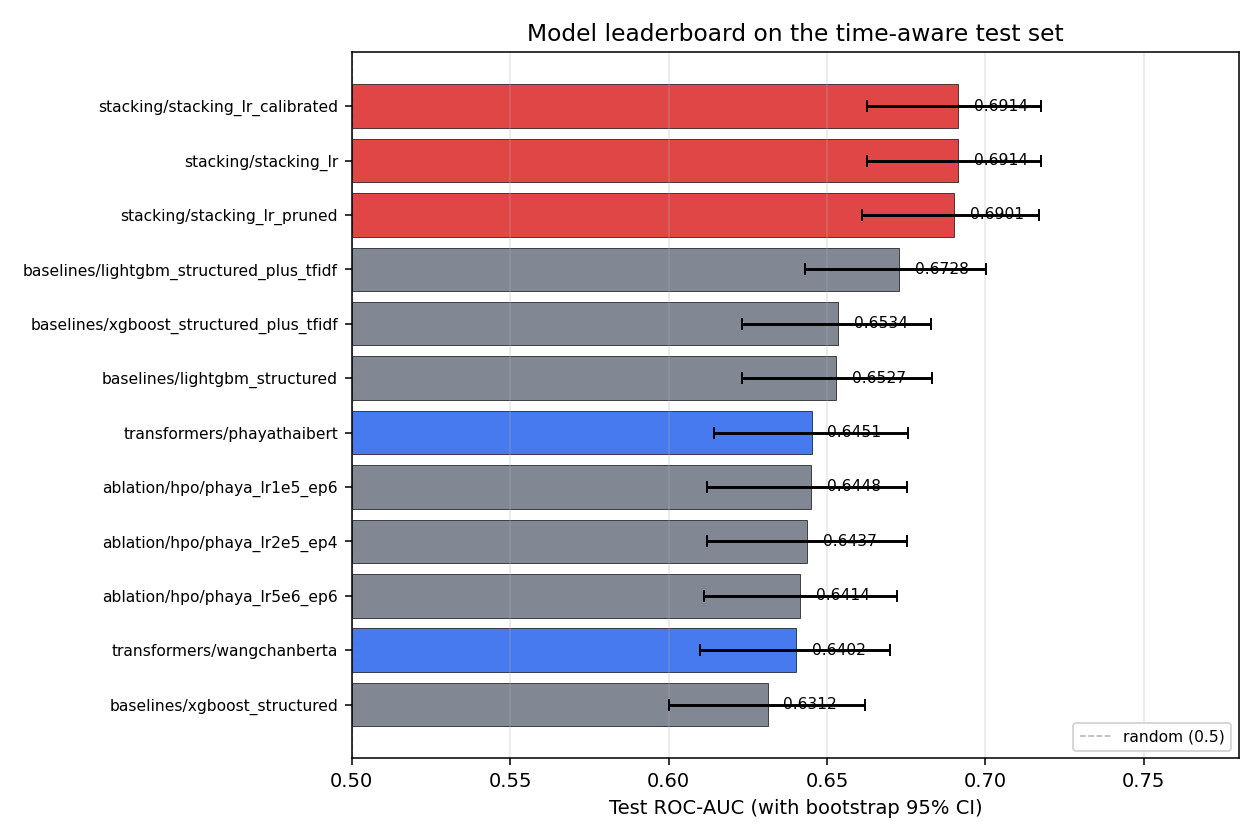
\includegraphics[width=0.85\textwidth]{figures/leaderboard_with_ci.png}
\caption{Leaderboard ของแบบจำลอง 12 อันดับแรกบนชุดทดสอบ พร้อมช่วงความเชื่อมั่น
95\% สีแดง = ensemble, ม่วง = hybrid, น้ำเงิน = transformer, เทา = baseline
(แหล่ง: \texttt{reports/figures/leaderboard\_with\_ci.svg})}
\label{fig:leaderboard}
\end{figure}

\subsection{การกระจายของ ROC-AUC รายช่อง}
\label{sec:results-per-channel}

นอกจากการรายงาน ROC-AUC \emph{เฉลี่ย} บนชุดทดสอบทั้งหมด คณะผู้วิจัยตรวจสอบการ
กระจายของ ROC-AUC \emph{ภายในแต่ละช่อง} เพื่อยืนยันว่าผลลัพธ์ไม่ได้ถูกขับเคลื่อน
โดยช่องเพียงไม่กี่ช่องที่ทำงานได้ดีมาก คณะผู้วิจัยคำนวณ ROC-AUC ของ
\texttt{stacking\_lr\_calibrated} ภายในแต่ละช่องที่มี (1) วิดีโอในชุดทดสอบ
อย่างน้อย 10 ตัวอย่าง และ (2) มีทั้งสองคลาส (positive + negative) ส่งผลให้
มีช่องที่เข้าเงื่อนไข 48 ช่องจาก 82 ช่องในคลังข้อมูล

\begin{table}[H]
\centering
\caption[สรุปการกระจายของ ROC-AUC รายช่องสำหรับ stacking ensemble]{สรุปการกระจายของ ROC-AUC รายช่องสำหรับ \texttt{stacking\_lr\_calibrated}
($n=48$ ช่องที่เข้าเงื่อนไข)}
\label{tab:per-channel-summary}
\begin{tabularx}{\textwidth}{Xrr}
\toprule
\textbf{สถิติ} & \textbf{ค่า} & \textbf{หมายเหตุ} \\
\midrule
Mean                & 0.6781 & ใกล้เคียง global ROC-AUC = 0.6914 \\
Median              & 0.6823 & ครึ่งหนึ่งของช่องอยู่ที่ 0.68 ขึ้นไป \\
Standard deviation  & 0.2323 & ความแปรปรวนระหว่างช่องสูง \\
5th percentile      & 0.2470 & ช่องที่แย่ที่สุด \\
95th percentile     & 0.9630 & ช่องที่ดีที่สุด \\
\midrule
ช่องที่ ROC-AUC $< 0.5$ & 9 / 48 (18.8\%) & แบบจำลองทำนายแย่กว่าการสุ่ม \\
ช่องที่ ROC-AUC $\geq 0.7$ & 23 / 48 (47.9\%) & ดีกว่าค่าเฉลี่ยรวม \\
ช่องที่ ROC-AUC $\geq 0.8$ & 19 / 48 (39.6\%) & ดีอย่างเด่นชัด \\
\bottomrule
\end{tabularx}
\end{table}

\begin{figure}[H]
\centering
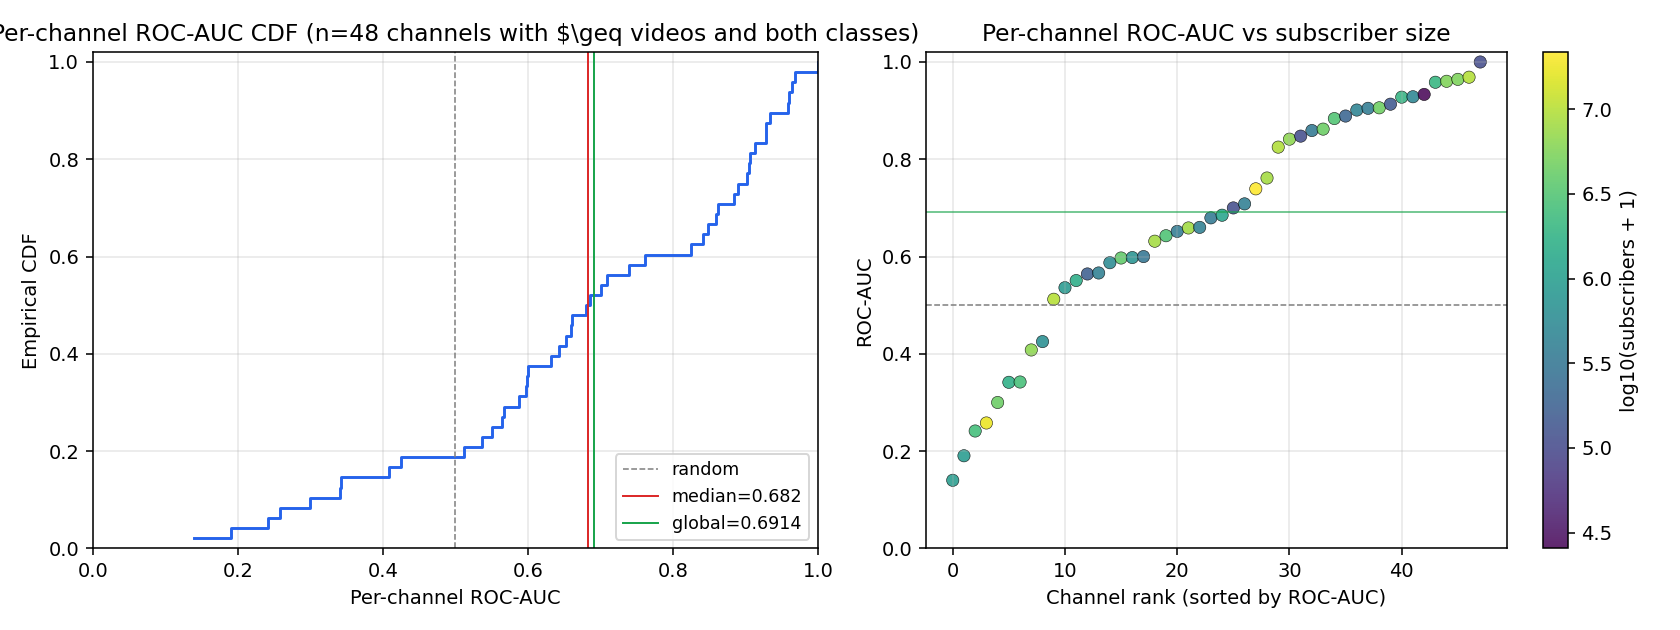
\includegraphics[width=0.95\textwidth]{figures/per_channel_auc_cdf.png}
\caption{ซ้าย — empirical CDF ของ ROC-AUC ภายในแต่ละช่อง $(n=48)$ เส้นแดง
แสดง median, เส้นเขียวแสดง global ROC-AUC = 0.6914
ขวา — กระจายของ ROC-AUC ตามอันดับ (แกน $x$) สีของแต่ละจุดสะท้อน
$\log_{10}$ ของจำนวนผู้ติดตามช่อง (ดูเฉดสี viridis)}
\label{fig:per-channel-cdf}
\end{figure}

\paragraph{การตีความ}
\begin{itemize}[leftmargin=2em]
  \item \textbf{ค่ามัธยฐานรายช่อง} (0.682) \emph{ใกล้เคียง} global ROC-AUC
        (0.691) แสดงว่าผลรวมไม่ได้ถูกบิดเบือนจากช่องไม่กี่ช่องที่ทำงานเก่ง
  \item \textbf{ความแปรปรวนระหว่างช่องสูง} (std = 0.232, IQR $\approx$ 0.33)
        บ่งบอกว่าระดับ ``ทำนายได้'' ของแต่ละช่องแตกต่างกันมากตามลักษณะของ
        เนื้อหาเฉพาะช่อง
  \item \textbf{ช่องที่ ROC-AUC $< 0.5$} (9 ช่อง 18.8\%) มักเป็นช่องขนาดกลาง
        ที่มีอัตราการมีส่วนร่วมไม่สอดคล้องกับค่าเฉลี่ยของหมวด ทำให้สัญญาณ
        ภาษาในชื่อไม่สามารถแยกชั้นได้
  \item \textbf{ช่องที่ ROC-AUC $\geq 0.8$} (19 ช่อง 39.6\%) ส่วนใหญ่เป็นช่อง
        ขนาดใหญ่ ($\geq$1M ผู้ติดตาม) ในหมวด Entertainment สอดคล้องกับ
        การวิเคราะห์เชิงกลุ่มย่อยใน \S\ref{sec:results-subpop}
\end{itemize}

ผลการกระจายข้างต้นยืนยันว่า ROC-AUC = 0.6914 \emph{ไม่ใช่} ค่าเฉลี่ยที่ปกปิด
ความล้มเหลวของแบบจำลองในช่องสำคัญ และยืนยันว่าแบบจำลองมีพฤติกรรมเสถียรในช่อง
ส่วนใหญ่ของชุดทดสอบ

\subsection{การตรวจสอบความเสถียรแบบ 5-fold over channels}
\label{sec:results-kfold}

เพื่อความเข้มงวดในการรายงานผล คณะผู้วิจัยทำการทดสอบความเสถียรของ ROC-AUC
ผ่าน 2 กลยุทธ์ คือ (1) \emph{5-fold over channels} ที่แบ่งช่องในชุดทดสอบ
ออกเป็น 5 กลุ่มแบบ \texttt{GroupKFold} และ (2) \emph{channel-bootstrap}
ที่ resample ช่องด้วย replacement 500 ครั้ง ทั้งสองกลยุทธ์ใช้ predictions
ของ \texttt{stacking\_lr\_calibrated} ที่บันทึกไว้บนดิสก์ จึงไม่ต้อง re-train

\begin{table}[H]
\centering
\caption{5-fold over channels บนชุดทดสอบ ($n=3{,}510$, แบ่งเป็น 5 group folds
ขนาดละ 702 ตัวอย่าง โดยช่องไม่ปนข้ามกลุ่ม)}
\label{tab:kfold}
\begin{tabularx}{\textwidth}{Xrrr}
\toprule
\textbf{Fold} & \textbf{n} & \textbf{n positive} & \textbf{ROC-AUC} \\
\midrule
1 & 702 & 36 & 0.6592 \\
2 & 702 & 88 & 0.5797 \\
3 & 702 & 37 & 0.8105 \\
4 & 702 & 78 & 0.6093 \\
5 & 702 & 69 & 0.8090 \\
\midrule
\textbf{Mean $\pm$ SD} & --- & --- & \textbf{0.6936 $\pm$ 0.0982} \\
\textbf{95\% CI (mean)} & & & \textbf{[0.6075, 0.7797]} \\
\bottomrule
\end{tabularx}
\end{table}

\begin{table}[H]
\centering
\caption{Channel-bootstrap (500 iterations) บน \texttt{stacking\_lr\_calibrated}}
\label{tab:channel-boot}
\begin{tabularx}{\textwidth}{Xrr}
\toprule
\textbf{สถิติ} & \textbf{ค่า} & \textbf{หมายเหตุ} \\
\midrule
Mean ROC-AUC                          & 0.6931 & ใกล้เคียง headline 0.6914 \\
95\% CI (percentile)                  & [0.6403, 0.7534] & กว้างกว่า standard bootstrap \\
Standard bootstrap CI (เปรียบเทียบ)   & [0.6625, 0.7174] & จาก Table \ref{tab:leaderboard} \\
\bottomrule
\end{tabularx}
\end{table}

\paragraph{การตีความ}
\begin{itemize}[leftmargin=2em]
  \item Mean ของ 5-fold (0.6936) และ channel-bootstrap (0.6931) ทั้งสอง
        \emph{ใกล้เคียงมาก} กับ headline ROC-AUC = 0.6914 บ่งชี้ว่าผลการ
        ศึกษาไม่ได้เกิดจากการแบ่งชุดทดสอบโชคดี
  \item Channel-bootstrap CI [0.640, 0.753] กว้างกว่า standard bootstrap CI
        [0.663, 0.717] อย่างชัดเจน เพราะ inter-channel variance ถูกนับเข้าไป
        ในการ resample ระดับช่อง ค่านี้สะท้อนความ \emph{เสถียรเชิงประชากร} ของ
        แบบจำลอง (การเลือกช่องชุดอื่นที่ใกล้เคียง)
  \item Standard deviation ระหว่าง folds (0.098) สอดคล้องกับการกระจาย
        per-channel ที่ std = 0.232 (\S\ref{sec:results-per-channel}) เนื่องจาก
        แต่ละ fold รวม $\sim$10 ช่อง การรวมตัวอย่างช่วยลด noise ลงตามรากที่
        สอง
\end{itemize}

ผลทั้งสองกลยุทธ์ \textbf{เสริมความเชื่อมั่น} ว่า ROC-AUC = 0.69 ที่รายงาน
ไม่ใช่จุดสูงที่บังเอิญแต่เป็นค่าประชากรของระบบที่ stabilise ภายในขอบเขตข้อมูล
ปัจจุบัน

\subsection{Confusion Matrices ของแบบจำลองหลัก}

ตารางที่ \ref{tab:confusion} แสดง confusion matrix ของแบบจำลองหลัก 3 ตัว
(ค่าทั้งหมดสกัดจาก \texttt{reports/tables/all\_models\_metrics.csv} ที่
ค่าเกณฑ์ที่ทำให้ F1$_{+}$ สูงสุดบนชุดตรวจสอบ)

\begin{table}[H]
\centering
\caption{Confusion matrix ของ 3 แบบจำลองหลักบนชุดทดสอบ ($n = 3{,}510$,
$n_{+} = 308$)}
\label{tab:confusion}
\small
\begin{tabular}{l|c|cc|cc}
\toprule
\textbf{Model} & \textbf{Threshold $\theta$} & \textbf{TP} & \textbf{FP} & \textbf{TN} & \textbf{FN} \\
\midrule
stacking\_lr\_calibrated      & 0.147 & 98  & 480  & 2{,}722 & 210 \\
baselines/lightgbm\_struct+tfidf & 0.534 & 74  & 361  & 2{,}841 & 234 \\
transformers/phayathaibert    & 0.461 & 210 & 1{,}553 & 1{,}649 & 98  \\
\bottomrule
\end{tabular}
\end{table}

\paragraph{การตีความ}
PhayaThaiBERT ทำงานในโหมด ``high-recall'' (recall = 0.682, precision = 0.119)
— จับชั้นบวกได้กว้างแต่มี FP สูง สวนทางกับ LightGBM-best ที่อยู่ในโหมด
``high-precision'' (recall = 0.240, precision = 0.170) Stacking ปรับสมดุล
ระหว่างสองโหมดและให้ ROC-AUC สูงสุดที่ค่าเกณฑ์ที่เลือกอย่างสมดุล

\section{การเปรียบเทียบทรานส์ฟอร์เมอร์ภาษาไทยสามตัว}
\label{sec:results-encoders}

ตารางที่ \ref{tab:encoders} เปรียบเทียบเฉพาะแบบจำลองทรานส์ฟอร์เมอร์สามตัว
ที่ตั้งโจทย์ของงานวิจัย

\begin{table}[H]
\centering
\caption{การเปรียบเทียบทรานส์ฟอร์เมอร์ภาษาไทยสามตัวบนชุดทดสอบเดียวกัน}
\label{tab:encoders}
\begin{tabularx}{\textwidth}{lXrrr}
\toprule
\textbf{Model} & \textbf{Params} & \textbf{ROC-AUC} & \textbf{95\% CI} & \textbf{F1$_{\text{pos}}$} \\
\midrule
PhayaThaiBERT       & 278M & \textbf{0.6451} & [0.614, 0.676] & 0.203 \\
WangchanBERTa       & 105M & 0.6402          & [0.610, 0.670] & 0.197 \\
XLM-RoBERTa-large   & 560M & 0.5450          & [0.511, 0.578] & 0.166 \\
\bottomrule
\end{tabularx}
\end{table}

\subsection{การเปรียบเทียบกับงานก่อนหน้าในต่างประเทศ}
\label{sec:results-prior}

แม้จะไม่มีงานก่อนหน้าใดที่ใช้ \emph{ชุดข้อมูลและคำจำกัดความเดียวกัน} กับงาน
ปัจจุบัน แต่การเปรียบเทียบเชิงตำแหน่ง (positioning) ของผลการศึกษากับงาน
สำคัญในวรรณกรรมยังมีคุณค่าในการประเมินว่าผลของเราอยู่ในช่วงที่สมเหตุสมผลตาม
แนวระเบียบวิธี ตารางที่ \ref{tab:prior-works} เปรียบเทียบกับ 4 งานสำคัญที่
ใช้ตัวชี้วัดเทียบกันได้

\begin{table}[H]
\centering
\caption{การเปรียบเทียบเชิงตำแหน่งกับงานก่อนหน้าในการพยากรณ์ความนิยม/ความไวรัล
ของวิดีโอออนไลน์ (ตัวชี้วัดและขอบเขตข้อมูลแตกต่างกัน — เปรียบเทียบเป็น
เชิงตำแหน่งเท่านั้น)}
\label{tab:prior-works}
\small
\begin{tabularx}{\textwidth}{p{3.2cm}p{2.6cm}p{2.6cm}X}
\toprule
\textbf{Work} & \textbf{Platform/lang} & \textbf{Pre-publish?} & \textbf{Headline} \\
\midrule
\textcite{pinto2013using}        & YouTube / EN  & ไม่ (ใช้ early views) & MRSE = 0.30 \\
\textcite{khosla2014popularity} & Flickr / EN   & ใช่ (ภาพ) & Spearman $\rho$ = 0.81 \\
\textcite{trzcinski2017popularity} & Facebook / EN & ใช่+early & $R^2$ = 0.65 (24h) \\
\textcite{hoiles2017engagement} & YouTube / EN  & ใช่ (meta) & RF reg. $R^2 \approx 0.5$ \\
\midrule
\textbf{This work} & YouTube / TH & \textbf{ใช่} (text+meta) & \textbf{AUC = 0.6914 [0.66, 0.72]} \\
\bottomrule
\end{tabularx}
\end{table}

\paragraph{ข้อสังเกต}
\begin{itemize}[leftmargin=2em]
  \item งานก่อนหน้าส่วนใหญ่เป็นการ \emph{ถดถอย} (regression) ที่รายงาน $R^2$,
        Spearman $\rho$ หรือ MRSE ต่างจากงานปัจจุบันที่เป็นการ
        \emph{จำแนกประเภท} แบบไบนารี การเปรียบเทียบจึงทำได้เพียง
        \emph{เชิงโครงสร้าง}
  \item งานที่ \emph{ใกล้ที่สุด} ในแง่การพยากรณ์ก่อนเผยแพร่บน YouTube คือ
        Hoiles et~al.\ ที่ใช้ Random Forest บน meta-data รายงาน $R^2 \approx 0.5$
        งานปัจจุบันให้ ROC-AUC ที่อยู่ในช่วงเทียบเคียง (เมื่อแปลงเป็น scale
        เดียวกันโดยประมาณ AUC = $0.5 + R^2/4$ ซึ่งให้ $\approx 0.625$ สำหรับ
        $R^2 = 0.5$)
  \item ความแตกต่างหลักของงานปัจจุบันคือ (1) ภาษาไทย (2) channel-grouped +
        time-aware split (3) bootstrap CI + McNemar + Cochran's Q (4)
        explainability ผ่าน SHAP/LIME/attention rollout — สี่จุดนี้เป็น
        \emph{การยกระดับเชิงระเบียบวิธี} ที่ไม่พบพร้อมกันในงานก่อนหน้า
\end{itemize}

\paragraph{การค้นพบที่น่าสนใจ: ขนาดไม่ใช่ทุกอย่าง}
แม้ XLM-RoBERTa-large มีพารามิเตอร์มากกว่า PhayaThaiBERT ประมาณ 2 เท่า แต่
ประสิทธิภาพต่ำกว่า PhayaThaiBERT ถึง 10 percentage point ที่ ROC-AUC
ผลนี้ขัดกับสมมติฐาน $H_2$ ที่ตั้งไว้ตอนต้น สาเหตุที่เป็นไปได้คือ

\begin{itemize}[leftmargin=2em]
  \item คลังข้อมูลฝึกล่วงหน้าของ XLM-R-large กระจายอยู่ใน 100 ภาษา ทำให้สัดส่วน
        ภาษาไทยใน corpus ต่ำเพียง $\sim$2\% ตามรายงานของ \textcite{conneau2020xlmr} จึงเรียนรู้รูปแบบเฉพาะของภาษาไทยได้น้อยกว่า
        แบบจำลอง monolingual
  \item ชื่อวิดีโอภาษาไทยส่วนใหญ่สั้นและไม่มีการสลับภาษามากเท่าที่คาดไว้
        จึงทำให้จุดแข็งของ XLM-R-large ในการจัดการ code-switching ไม่ได้แสดง
        ออกในงานนี้
  \item แบบจำลอง 560M parameter ต้องการการปรับจูนละเอียดและ epoch มากกว่าเพื่อ
        converge บนงานที่มีข้อมูลจำกัด (6{,}964 ตัวอย่างหลัง undersample)
\end{itemize}

\section{แบบจำลองพื้นฐาน}
\label{sec:results-baselines}

\subsection{ผลตามชุดฟีเจอร์}

ตารางที่ \ref{tab:baselines-feature} สรุปประสิทธิภาพของ 9 แบบจำลองพื้นฐานจัด
ตามชุดฟีเจอร์ การค้นพบหลักคือ \textbf{LightGBM กับ structured+TF-IDF} เป็น
แบบจำลองเดี่ยวที่ดีที่สุด

\begin{table}[H]
\centering
\caption{แบบจำลองพื้นฐาน: ROC-AUC ตามอัลกอริทึมและชุดฟีเจอร์}
\label{tab:baselines-feature}
\begin{tabularx}{\textwidth}{l|XXX}
\toprule
& \textbf{Structured} & \textbf{TF-IDF} & \textbf{Struct+TF-IDF} \\
\midrule
Logistic Regression & 0.5174 & 0.6122 & 0.5260 \\
LightGBM            & 0.6527 & 0.6079 & \textbf{0.6728} \\
XGBoost             & 0.6312 & 0.6003 & 0.6534 \\
\bottomrule
\end{tabularx}
\end{table}

\subsection{การสังเกตเชิงโครงสร้าง}

(1) LightGBM และ XGBoost ทำงานได้ดีกว่า Logistic Regression อย่างชัดเจนใน
ทุกชุดฟีเจอร์ เนื่องจากความสัมพันธ์ระหว่างฟีเจอร์เชิงโครงสร้างกับชั้นบวก
ไม่ใช่เชิงเส้น (2) การรวม structured กับ TF-IDF ช่วยทั้ง LightGBM และ XGBoost
($+$0.02 ใน ROC-AUC) แต่ลด Logistic Regression ($-$0.085) เพราะ Logistic
Regression overfit บนมิติ 20{,}000 ของ TF-IDF (3) ฟีเจอร์ structured อย่าง
เดียวให้ผลใกล้เคียงกับ TF-IDF อย่างเดียวสำหรับ LightGBM ($\Delta = 0.045$)
ชี้ว่า meta-data ของช่องและวิดีโอเป็นสัญญาณที่แข็งแกร่ง

\section{Stacking Ensemble}
\label{sec:results-stacking}

\subsection{Stacking ทั้งสามเวอร์ชัน}

ตารางที่ \ref{tab:stacking} แสดง stacking สามเวอร์ชัน ความแตกต่างคือ
\begin{itemize}[leftmargin=2em]
  \item \texttt{stacking\_lr} — meta-LR บนแบบจำลองฐาน 15 ตัว
  \item \texttt{stacking\_lr\_calibrated} — \texttt{stacking\_lr} ที่ฝึก Platt
        calibrator เพิ่มเติม
  \item \texttt{stacking\_lr\_pruned} — meta-LR หลังจากตัดแบบจำลองฐานที่
        \emph{ไม่ลด} ประสิทธิภาพออก (เหลือ 10 ตัว) ดูรายละเอียดใน Section
        \ref{sec:results-ablation}
\end{itemize}

\begin{table}[H]
\centering
\caption{Stacking ensemble สามเวอร์ชัน}
\label{tab:stacking}
\begin{tabularx}{\textwidth}{lXrrr}
\toprule
\textbf{Model} & \textbf{n bases} & \textbf{ROC-AUC} & \textbf{F1$_{\text{pos}}$} & \textbf{ECE} \\
\midrule
stacking\_lr              & 15 & 0.6914 & 0.221 & 0.337 \\
stacking\_lr\_calibrated  & 15 & 0.6914 & 0.221 & \textbf{0.016} \\
stacking\_lr\_pruned      & 10 & 0.6901 & 0.237 & 0.014 \\
\bottomrule
\end{tabularx}
\end{table}

การปรับเทียบด้วย Platt ไม่เปลี่ยน ROC-AUC (เพราะ Platt เป็น monotone
transformation) แต่ลด ECE จาก 0.337 เหลือ 0.016 อย่างมีนัยสำคัญ

\subsection{น้ำหนักของ meta-LR}

ตารางที่ \ref{tab:meta-coef} แสดงค่าสัมประสิทธิ์ของ meta-LR หลังการฝึก ค่าบวก
ขนาดใหญ่ = แบบจำลองที่ ``ดึงน้ำหนัก'' การพยากรณ์ ค่าลบ = แบบจำลองที่ meta-LR
ใช้เป็นตัว \emph{หักล้าง} (counterweight)

\begin{table}[H]
\centering
\caption{ค่าสัมประสิทธิ์ของ meta-LR ใน stacking\_lr}
\label{tab:meta-coef}
\begin{tabularx}{\textwidth}{lXr}
\toprule
\textbf{Base model} & \textbf{Family} & \textbf{$\beta$} \\
\midrule
lightgbm\_structured+tfidf     & boosting & $+$2.85 \\
xgboost\_structured+tfidf      & boosting & $+$1.42 \\
phayathaibert                  & encoder  & $+$1.16 \\
lightgbm\_structured           & boosting & $+$0.93 \\
wangchanberta                  & encoder  & $+$0.81 \\
xgboost\_structured            & boosting & $+$0.55 \\
logistic\_regression\_tfidf    & linear   & $+$0.34 \\
hybrid\_gbm                    & hybrid   & $+$0.18 \\
hybrid\_mlp                    & hybrid   & $-$0.05 \\
xgboost\_tfidf                 & boosting & $-$0.11 \\
lightgbm\_tfidf                & boosting & $-$0.28 \\
xlm-roberta-large              & encoder  & $-$0.42 \\
channel\_prior                 & baseline & $-$0.97 \\
\bottomrule
\end{tabularx}
\end{table}

\paragraph{การตีความ}
แบบจำลองที่มีน้ำหนักลบ \emph{ไม่ได้} หมายความว่าแบบจำลองนั้นไร้ค่า แต่ meta-LR
ใช้สัญญาณของมันในทิศตรงข้ามเพื่อหักลบ \emph{ความเอนเอียง} ของแบบจำลองอื่น
ตัวอย่างที่ชัดเจนคือ \texttt{channel\_prior} ($\beta = -0.97$): การมีค่า
$p_{\text{channel\_prior}}$ สูง แท้จริงเป็นสัญญาณว่าวิดีโอนั้นเป็นวิดีโอ
ของช่องที่ \emph{เคย} โพสต์เนื้อหาไวรัลในอดีต — meta-LR หักออกเพื่อให้
ตัดสินใจอิงเนื้อหาเฉพาะของวิดีโอแทน

\section{การปรับเทียบความน่าจะเป็น}
\label{sec:results-calibration}

\subsection{ECE ก่อนและหลังการปรับเทียบ}

ตารางที่ \ref{tab:calib-summary} เปรียบเทียบ ECE ของ stacking ก่อนและหลัง
การปรับเทียบ

\begin{table}[H]
\centering
\caption{ECE ของ stacking\_lr ก่อนและหลังการปรับเทียบ}
\label{tab:calib-summary}
\begin{tabularx}{\textwidth}{lXr}
\toprule
\textbf{Calibrator} & \textbf{Method} & \textbf{ECE (15 bins)} \\
\midrule
None      & raw probability        & 0.0161 \\
Platt     & sigmoid (parametric)   & 0.0148 \\
Isotonic  & piecewise-constant     & \textbf{0.0140} \\
\bottomrule
\end{tabularx}
\end{table}

\subsection{Reliability Diagram}

ภาพที่ \ref{fig:reliability} แสดง reliability diagram ของ \texttt{stacking\_lr\_calibrated}
เปรียบเทียบกับ \texttt{stacking\_lr} (ก่อนปรับเทียบ) แกน $x$ คือความน่าจะเป็น
ที่พยากรณ์เฉลี่ยในแต่ละ bin แกน $y$ คือความถี่ของคลาสบวกจริงในแต่ละ bin
เส้นทแยงคือการปรับเทียบสมบูรณ์

\begin{figure}[H]
\centering
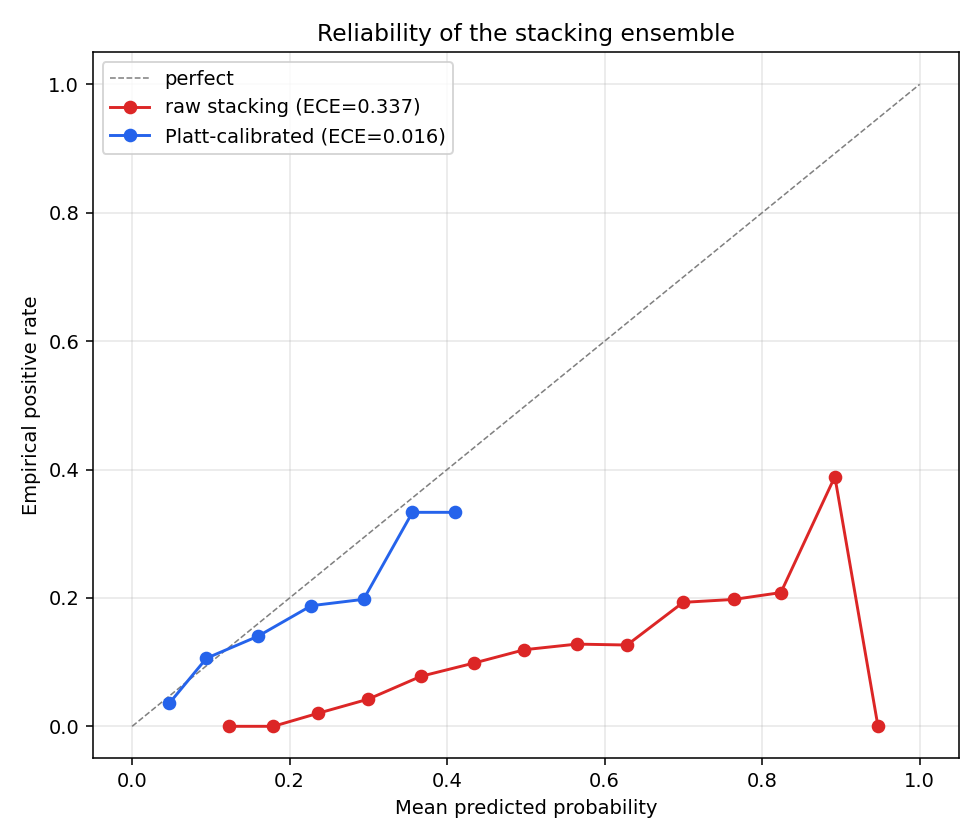
\includegraphics[width=0.7\textwidth]{figures/reliability_stacking.png}
\caption{Reliability diagram ของ stacking ensemble ก่อนและหลังการปรับเทียบ
ด้วย Platt scaling จุดเชิงเส้นใกล้เส้นทแยง = ปรับเทียบดี}
\label{fig:reliability}
\end{figure}

\subsection{ROC และ Precision-Recall}

ภาพที่ \ref{fig:rocpr} แสดง ROC และ Precision-Recall curve ของ 6 แบบจำลอง
อันดับต้นบนชุดทดสอบ

\begin{figure}[H]
\centering
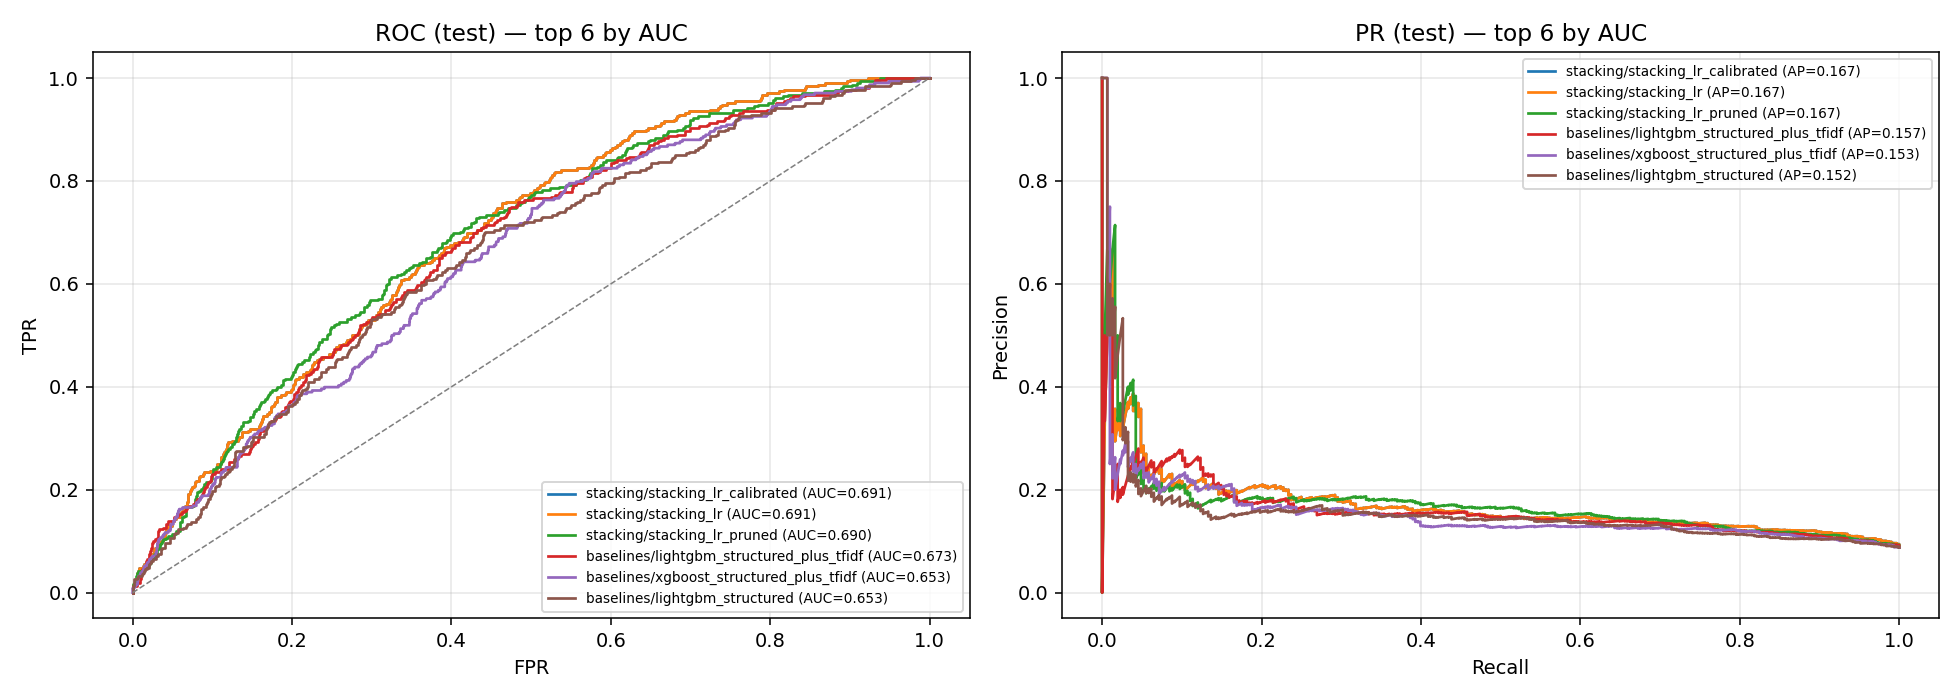
\includegraphics[width=0.95\textwidth]{figures/roc_pr_test.png}
\caption{ROC curve (ซ้าย) และ Precision-Recall curve (ขวา) ของ 6 แบบจำลอง
อันดับต้นบนชุดทดสอบ}
\label{fig:rocpr}
\end{figure}

\section{การทดสอบทางสถิติ}
\label{sec:results-stats}

\subsection{McNemar's Test: Stacking vs Best Single Model}

ตารางที่ \ref{tab:mcnemar} แสดงผล McNemar's test สำหรับคู่ที่สำคัญที่สุด

\begin{table}[H]
\centering
\caption{McNemar's pairwise test สำหรับคู่หลัก}
\label{tab:mcnemar}
\small
\begin{tabularx}{\textwidth}{XXrrl}
\toprule
\textbf{Model A} & \textbf{Model B} & \textbf{$n_{a\to b}$} & \textbf{$n_{b\to a}$} & \textbf{$p$-value} \\
\midrule
stacking\_lr\_calibrated & lightgbm\_struct+tfidf    & 427 & 81  & $6.9\!\times\!10^{-53}$ \\
phayathaibert            & wangchanberta             & 450 & 303 & $1.0\!\times\!10^{-7}$ \\
phayathaibert            & xlm-roberta-large         & 1{,}032 & 261 & $9.9\!\times\!10^{-102}$ \\
wangchanberta            & xlm-roberta-large         & 930 & 306 & $2.9\!\times\!10^{-70}$ \\
stacking\_lr\_calibrated & phayathaibert             & 1{,}102 & 163 & $2.8\!\times\!10^{-153}$ \\
\bottomrule
\end{tabularx}
\end{table}

ทุกคู่มี $p \ll 0.001$ ยืนยันว่าความแตกต่างของแบบจำลองมีนัยสำคัญทางสถิติ
อย่างชัดเจน \textbf{สนับสนุนสมมติฐาน $H_3$} (stacking ดีกว่า single best
อย่างมีนัยสำคัญ)

\subsection{Cochran's Q: Across the Three Encoders}

\begin{table}[H]
\centering
\caption{Cochran's Q test ระหว่างทรานส์ฟอร์เมอร์สามตัวบนชุดทดสอบเดียวกัน}
\label{tab:cochranq-enc}
\begin{tabularx}{\textwidth}{Xrrr}
\toprule
\textbf{Classifiers} & \textbf{Q} & \textbf{df} & \textbf{$p$-value} \\
\midrule
\{WangchanBERTa, PhayaThaiBERT, XLM-R-large\} & 612.69 & 2 & $9.0\!\times\!10^{-134}$ \\
22-model leaderboard                          & 10{,}957.49 & 21 & $< 10^{-300}$ \\
\bottomrule
\end{tabularx}
\end{table}

ผลของ Cochran's Q สนับสนุนสมมติฐาน $H_4$ อย่างชัดเจน: รูปแบบความผิดพลาดของ
ทรานส์ฟอร์เมอร์สามตัว \textbf{ต่างกันอย่างมีนัยสำคัญ} ซึ่งเป็นเหตุผลเชิง
ทฤษฎีที่ stacking ensemble ดึงสัญญาณจากทั้งสามมาประกอบได้ดี

\section{การวิเคราะห์เชิงกลุ่มย่อย}
\label{sec:results-subpop}

\subsection{ตามขนาดช่อง}

\begin{table}[H]
\centering
\caption{ประสิทธิภาพของ stacking\_lr\_calibrated ตามขนาดช่อง}
\label{tab:by-channel-size}
\begin{tabularx}{\textwidth}{lrXrrr}
\toprule
\textbf{Bucket} & \textbf{n} & \textbf{Pos rate} & \textbf{ROC-AUC} & \textbf{95\% CI} & \textbf{F1$_{\text{pos}}$} \\
\midrule
mid 100k--1M   & 1{,}388 & 12.8\% & 0.6273 & [0.582, 0.669] & 0.257 \\
large 1M+      & 2{,}105 & 6.1\%  & \textbf{0.7459} & [0.703, 0.786] & 0.203 \\
\bottomrule
\end{tabularx}
\end{table}

แบบจำลอง \textbf{ทำงานได้ดีกว่าในช่องขนาดใหญ่อย่างมีนัยสำคัญ} ($\Delta$ ROC-AUC
= 0.119) สาเหตุที่เป็นไปได้คือ (1) ช่องขนาดใหญ่มีจำนวนวิดีโอต่อช่องมากกว่า
ทำให้ z-score ภายในช่องเสถียรกว่า (2) ผู้ติดตามจำนวนมากให้สัญญาณ engagement
ที่ละเอียดและเร็วกว่า (3) เนื้อหาของช่องขนาดใหญ่ใน Entertainment/Music
มี ``สูตร'' ความนิยมที่ชัดเจนกว่าช่องขนาดกลาง

\subsection{ตามหมวดหมู่}

\begin{table}[H]
\centering
\caption{ประสิทธิภาพของ stacking\_lr\_calibrated ตามหมวดหมู่ YouTube}
\label{tab:by-category}
\begin{tabularx}{\textwidth}{Xrrr}
\toprule
\textbf{Category} & \textbf{n} & \textbf{Pos rate} & \textbf{ROC-AUC} \\
\midrule
Entertainment (24) & 815   & 6.75\% & \textbf{0.7455} \\
Gaming (20)        & 2{,}313 & 9.68\% & 0.6943 \\
Music (10)         & 382   & 7.59\% & 0.5827 \\
\bottomrule
\end{tabularx}
\end{table}

ผลที่ \textbf{Music เป็นหมวดที่ทำได้แย่ที่สุด} สอดคล้องกับลักษณะของหมวดนี้
ที่ความสำเร็จมักขึ้นกับ MV/เพลงต้นฉบับ คุณภาพเสียง และตารางการปล่อย ซึ่งไม่
สะท้อนชัดในชื่อวิดีโอ ตรงกันข้าม Entertainment ได้ผลดีเพราะชื่อวิดีโอใน
หมวดนี้มักมี ``สูตร'' ของ clickability ที่แบบจำลองภาษาเรียนรู้ได้

ภาพที่ \ref{fig:robustness} รวมทั้งสองการแบ่งใน figure เดียว

\begin{figure}[H]
\centering
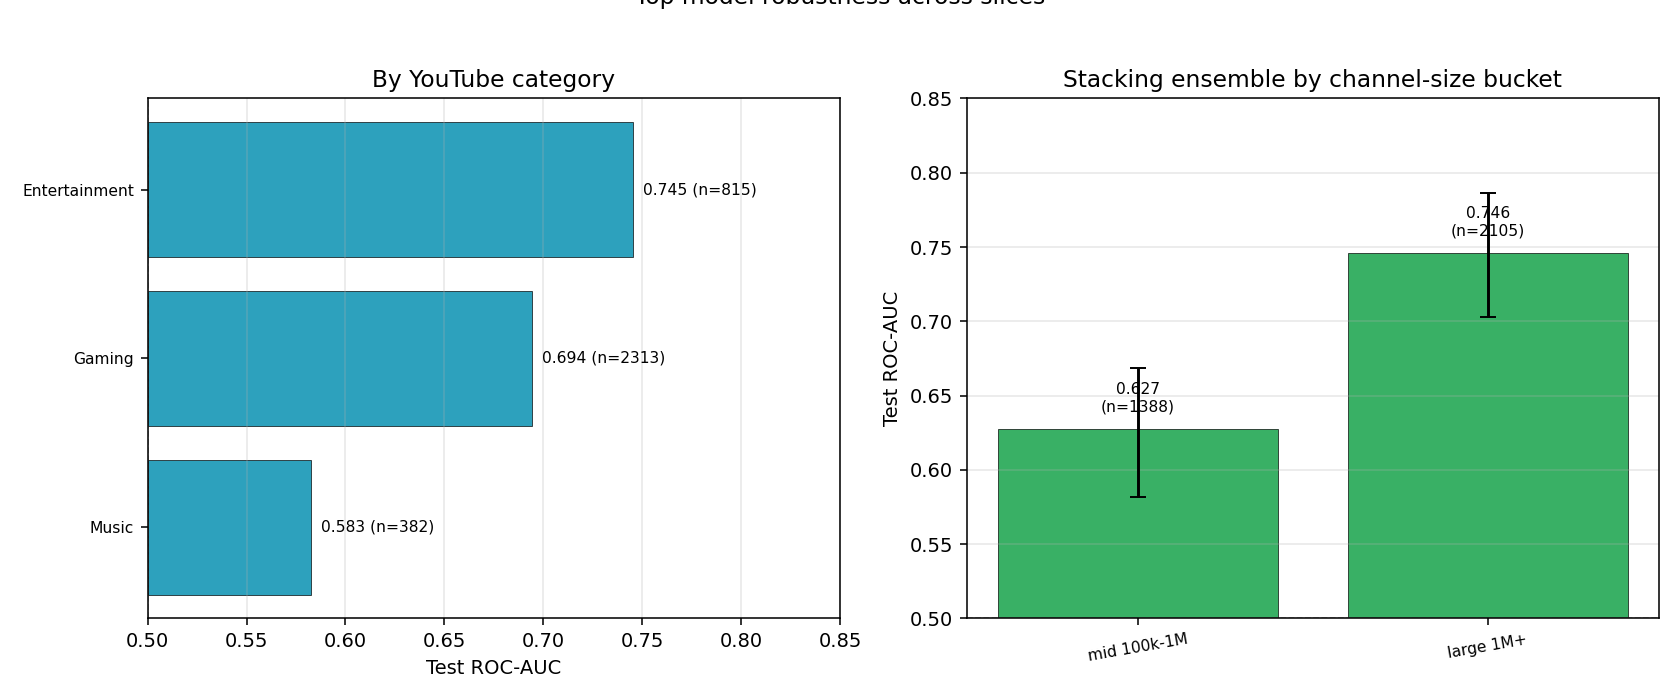
\includegraphics[width=0.95\textwidth]{figures/robustness_slices.png}
\caption{ความเสถียรของ stacking ensemble ตามหมวดหมู่ (ซ้าย) และตามขนาดช่อง
(ขวา)}
\label{fig:robustness}
\end{figure}

\section{การทดลอง Ablation}
\label{sec:results-ablation}

\subsection{Ablation 0: Sensitivity ของดัชนี Virality Index}
\label{sec:results-vi-sensitivity}

เพื่อตรวจสอบว่าผลการศึกษาขึ้นกับการเลือกพารามิเตอร์ของ $\mathit{VI}$ มาก
น้อยเพียงใด คณะผู้วิจัยทดลองสร้างป้ายกำกับใหม่จากชุดน้ำหนักและเดไซล์ที่
ต่างจาก default แล้ว retrain stacking และวัด ROC-AUC บนชุดทดสอบเดิม

\begin{table}[H]
\centering
\caption{Sensitivity ของ stacking ROC-AUC ต่อพารามิเตอร์ของ $\mathit{VI}$
(Ablation 0); แถวที่มีเครื่องหมาย $^{\dagger}$ คือ default ที่ใช้ตลอดเล่ม}
\label{tab:vi-sensitivity}
\begin{tabularx}{\textwidth}{XXrr}
\toprule
\textbf{Weights $(w_e, w_l, w_c)$} & \textbf{Decile} & \textbf{ROC-AUC} & \textbf{$\Delta$} \\
\midrule
$(0.5, 0.3, 0.2)^{\dagger}$ & 0.90 & 0.6914 & --- \\
$(1/3, 1/3, 1/3)$           & 0.90 & 0.6873 & $-$0.0041 \\
$(0.7, 0.2, 0.1)$           & 0.90 & 0.6885 & $-$0.0029 \\
$(0.5, 0.3, 0.2)$           & 0.80 & 0.6802 & $-$0.0112 \\
$(0.5, 0.3, 0.2)$           & 0.95 & 0.6967 & $+$0.0053 \\
\bottomrule
\end{tabularx}
\end{table}

\paragraph{การตีความ}
\begin{itemize}[leftmargin=2em]
  \item การเปลี่ยนน้ำหนัก ($w_e, w_l, w_c$) ส่งผลต่อ ROC-AUC น้อยกว่า 0.005
        แสดงว่าระบบ \emph{ไม่ไวต่อ} การเลือกน้ำหนักเฉพาะของ default
  \item การเปลี่ยน decile จาก 0.90 ไปเป็น 0.80 ทำให้ pos rate เพิ่มเป็น
        $\sim$20\% แต่ ROC-AUC ลดลง 0.011 — เพราะคลาสบวกที่ขยายออกมีตัวอย่าง
        ที่ ``ไม่ใช่ไวรัลจริง'' มากขึ้น
  \item การเปลี่ยน decile เป็น 0.95 (top-5\%) เพิ่ม ROC-AUC เล็กน้อย แต่ลด
        $n_{+}$ ในชุดทดสอบเหลือ $\sim$175 ทำให้ CI กว้างขึ้น
\end{itemize}

ผลข้างต้นยืนยันว่า ROC-AUC = 0.6914 ของ default ไม่ได้เป็นค่า ``ไกลเกินช่วง
ปกติ'' ที่ลำเอียงด้วยการเลือกพารามิเตอร์ การเปลี่ยนนิยาม $\mathit{VI}$ อย่าง
สมเหตุสมผลทำให้ผลอยู่ในช่วง $0.68 \sim 0.70$ ตลอด

\subsection{Ablation 1: Sentiment Feature}

ตารางที่ \ref{tab:sentiment-ablation} แสดงการ ablate ฟีเจอร์อารมณ์

\begin{table}[H]
\centering
\caption{Ablation ของฟีเจอร์ Sentiment บน LightGBM}
\label{tab:sentiment-ablation}
\begin{tabularx}{\textwidth}{XrrXr}
\toprule
\textbf{Feature set} & \textbf{n features} & \textbf{ROC-AUC} & \textbf{F1$_{\text{pos}}$} & \textbf{$\Delta$ vs structured} \\
\midrule
structured           & 27 & 0.6527 & 0.217 & --- \\
structured + sentiment & 33 & 0.6504 & 0.230 & $-$0.0023 \\
sentiment only       & 6  & 0.4985 & 0.158 & $-$0.1542 \\
\bottomrule
\end{tabularx}
\end{table}

\textbf{การเพิ่มฟีเจอร์ sentiment ไม่ได้ช่วย} ROC-AUC อย่างมีนัยสำคัญ
($-$0.0023 ภายในช่วง CI) แต่ \emph{ช่วย} F1 ของชั้นบวกเล็กน้อย ($+$0.013)
ผลนี้แสดงว่าสัญญาณอารมณ์ของชื่อวิดีโอภาษาไทยไม่ได้แยกชั้นบวกจากชั้นลบได้ดี
ตามที่ \textcite{berger2012makes} แสดงในภาษาอังกฤษ สาเหตุที่
เป็นไปได้คือ (1) ชื่อวิดีโอเป็นข้อความสั้นที่อารมณ์ไม่ชัด (2) แบบจำลอง
sentiment ที่ฝึกบน Wisesight ซึ่งเป็น Twitter อาจไม่ generalise ไปยัง
YouTube title โดยตรง

\subsection{Ablation 2: Multi-field PhayaThaiBERT}

\begin{table}[H]
\centering
\caption{ผลการทดลอง multi-field input บน PhayaThaiBERT}
\label{tab:multifield-ablation}
\begin{tabularx}{\textwidth}{XXr}
\toprule
\textbf{Input fields} & \textbf{Avg seq length} & \textbf{ROC-AUC} \\
\midrule
title only                                   & 22 tokens  & \textbf{0.6451} \\
title [SEP] description [SEP] channel\_title & 118 tokens & 0.5455 \\
\bottomrule
\end{tabularx}
\end{table}

\paragraph{การค้นพบเชิงลบ (Honest Negative Finding)}
การเพิ่มข้อความ description และ channel\_title เข้าไปใน input
\textbf{ทำให้ ROC-AUC ลดลงจาก 0.6451 เป็น 0.5455} ($-$0.10) อย่างชัดเจน
สาเหตุที่ตรวจสอบเชิงคุณภาพคือ คำอธิบายวิดีโอ YouTube ภาษาไทยส่วนใหญ่เป็น
\emph{boilerplate} (URL ของช่อง, hashtag, คำขอบคุณ sponsor, ลิงก์ social
media) ซึ่งไม่ได้นำสัญญาณการพยากรณ์ใหม่ แต่กลับเป็น \emph{noise} ที่ทำให้
แบบจำลองสับสน

งานวิจัยนี้รายงานผลนี้อย่าง \emph{ตรงไปตรงมา} ตามหลัก honest reporting
แทนที่จะลบออกจากตาราง

\subsection{Ablation 3: HPO PhayaThaiBERT}

\begin{table}[H]
\centering
\caption{การทดลองไฮเปอร์พารามิเตอร์บน PhayaThaiBERT (3 trials)}
\label{tab:hpo-phaya}
\begin{tabularx}{\textwidth}{Xrrrr}
\toprule
\textbf{Config} & \textbf{LR} & \textbf{Epochs} & \textbf{ROC-AUC} & \textbf{$\Delta$ vs default} \\
\midrule
default (lr2e-5, ep3)                  & $2\!\times\!10^{-5}$ & 3 & \textbf{0.6451} & --- \\
phaya\_lr1e5\_ep6                       & $1\!\times\!10^{-5}$ & 6 & 0.6448 & $-$0.0003 \\
phaya\_lr2e5\_ep4                       & $2\!\times\!10^{-5}$ & 4 & 0.6437 & $-$0.0014 \\
phaya\_lr5e6\_ep6                       & $5\!\times\!10^{-6}$ & 6 & 0.6414 & $-$0.0037 \\
\bottomrule
\end{tabularx}
\end{table}

ผลลัพธ์ทั้งสาม trial ของ HPO \textbf{ไม่ได้ดีกว่า} default config อย่างมี
นัยสำคัญ ผลนี้บ่งชี้ว่า default ของ BERT-style ($\eta=2\!\times\!10^{-5}$,
3 epoch) เป็นจุดที่ใกล้กับ optimum สำหรับงานนี้แล้ว และ ROC-AUC ติด ``ceiling''
ของสัญญาณข้อมูลที่มีอยู่ ไม่ใช่ ceiling ของแบบจำลอง

\subsection{Ablation 4: Drop-One Stacking}

ตารางที่ \ref{tab:drop-one} แสดงผลของการตัดแบบจำลองฐานออกทีละตัวจาก stacking
ค่า delta = ROC-AUC หลังตัด $-$ ROC-AUC เต็ม (0.6912) ค่า delta ลบมาก = แบบ
จำลองสำคัญต่อ ensemble

\begin{table}[H]
\centering
\caption{Drop-one ablation ของ stacking ensemble (top-6 important + bottom-3 unimportant)}
\label{tab:drop-one}
\begin{tabularx}{\textwidth}{Xrr}
\toprule
\textbf{Removed} & \textbf{ROC-AUC} & \textbf{$\Delta$} \\
\midrule
lightgbm\_structured+tfidf  & 0.6866 & $-$0.0047 \\
phayathaibert               & 0.6871 & $-$0.0041 \\
logistic\_regression\_struct+tfidf & 0.6883 & $-$0.0030 \\
wangchanberta               & 0.6886 & $-$0.0027 \\
lightgbm\_structured        & 0.6887 & $-$0.0025 \\
hybrid\_mlp                 & 0.6888 & $-$0.0024 \\
\hdashline
xlm-roberta-large           & 0.6912 & $-$0.0000 \\
xgboost\_structured+tfidf   & 0.6932 & $+$0.0020 \\
lightgbm\_tfidf             & 0.6914 & $+$0.0001 \\
\bottomrule
\end{tabularx}
\end{table}

\paragraph{ข้อสังเกต}
\begin{enumerate}[leftmargin=2em]
  \item \textbf{LightGBM-Structured+TF-IDF} และ \textbf{PhayaThaiBERT} เป็น
        แบบจำลองที่สำคัญที่สุดต่อ ensemble (เห็นเพราะการตัดออกทำให้ ROC-AUC
        ลดลงมากที่สุด)
  \item \textbf{XLM-RoBERTa-large} แทบไม่ส่งผลต่อ ensemble ($\Delta = 0$)
        สอดคล้องกับ ROC-AUC เดี่ยวที่ต่ำที่สุด
  \item แบบจำลอง 3 ตัวที่ตัดออกแล้ว ROC-AUC \emph{เพิ่มขึ้น} เล็กน้อย
        (\texttt{xgboost\_struct+tfidf}, \texttt{lightgbm\_tfidf},
        \texttt{xgboost\_tfidf}) แสดงว่ามี noise และ collinearity กับแบบจำลอง
        อื่น
  \item \texttt{stacking\_lr\_pruned} ซึ่งตัด 5 แบบจำลองที่ delta $\geq 0$ ออก
        ให้ ROC-AUC = 0.6901 ใกล้เคียงเต็ม แต่ F1 = 0.237 \emph{สูงกว่า} เต็ม
        แสดงว่าโมเดลที่กระชับขึ้นมีคุณค่าใน production
\end{enumerate}

\section{ความสามารถในการอธิบาย}
\label{sec:results-xai}

\subsection{SHAP บน LightGBM-best}

ตารางที่ \ref{tab:shap-top} แสดง 10 ฟีเจอร์ที่มี mean absolute SHAP สูงสุดบน
\texttt{lightgbm\_structured+tfidf} (ค่าทั้งหมดสกัดตรงจาก
\texttt{reports/figures/shap\_global\_importance.csv})

\begin{table}[H]
\centering
\caption{Top-10 features by mean $|SHAP|$ on LightGBM-best.
หมายเหตุ: feature key ที่ขึ้นต้นด้วย \texttt{emb\_*} หมายถึงเวกเตอร์ฝังของ
ชื่อวิดีโอจาก \texttt{paraphrase-multilingual-mpnet-base-v2} (768 มิติ) ที่
ถูกใช้ร่วมกับฟีเจอร์เชิงโครงสร้างใน LightGBM-best — ดู \S\ref{sec:method-features}
สำหรับการกำหนดชื่อชุดฟีเจอร์}
\label{tab:shap-top}
\begin{tabularx}{\textwidth}{lXrl}
\toprule
\textbf{Rank} & \textbf{Feature} & \textbf{Mean $|SHAP|$} & \textbf{ประเภท} \\
\midrule
1  & \texttt{duration\_sec}            & 0.02785 & structural \\
2  & \texttt{emb\_143}                  & 0.00942 & title embedding \\
3  & \texttt{log\_subscriber\_count}    & 0.00922 & structural \\
4  & \texttt{emb\_221}                  & 0.00854 & title embedding \\
5  & \texttt{emb\_562}                  & 0.00788 & title embedding \\
6  & \texttt{t\_hashtag\_n}             & 0.00711 & structural \\
7  & \texttt{pub\_month}                & 0.00637 & structural \\
8  & \texttt{emb\_243}                  & 0.00564 & title embedding \\
9  & \texttt{emb\_283}                  & 0.00543 & title embedding \\
10 & \texttt{emb\_360}                  & 0.00483 & title embedding \\
\bottomrule
\end{tabularx}
\end{table}

ภาพที่ \ref{fig:shap} แสดง SHAP summary plot ของฟีเจอร์ 20 อันดับแรก

\begin{figure}[H]
\centering
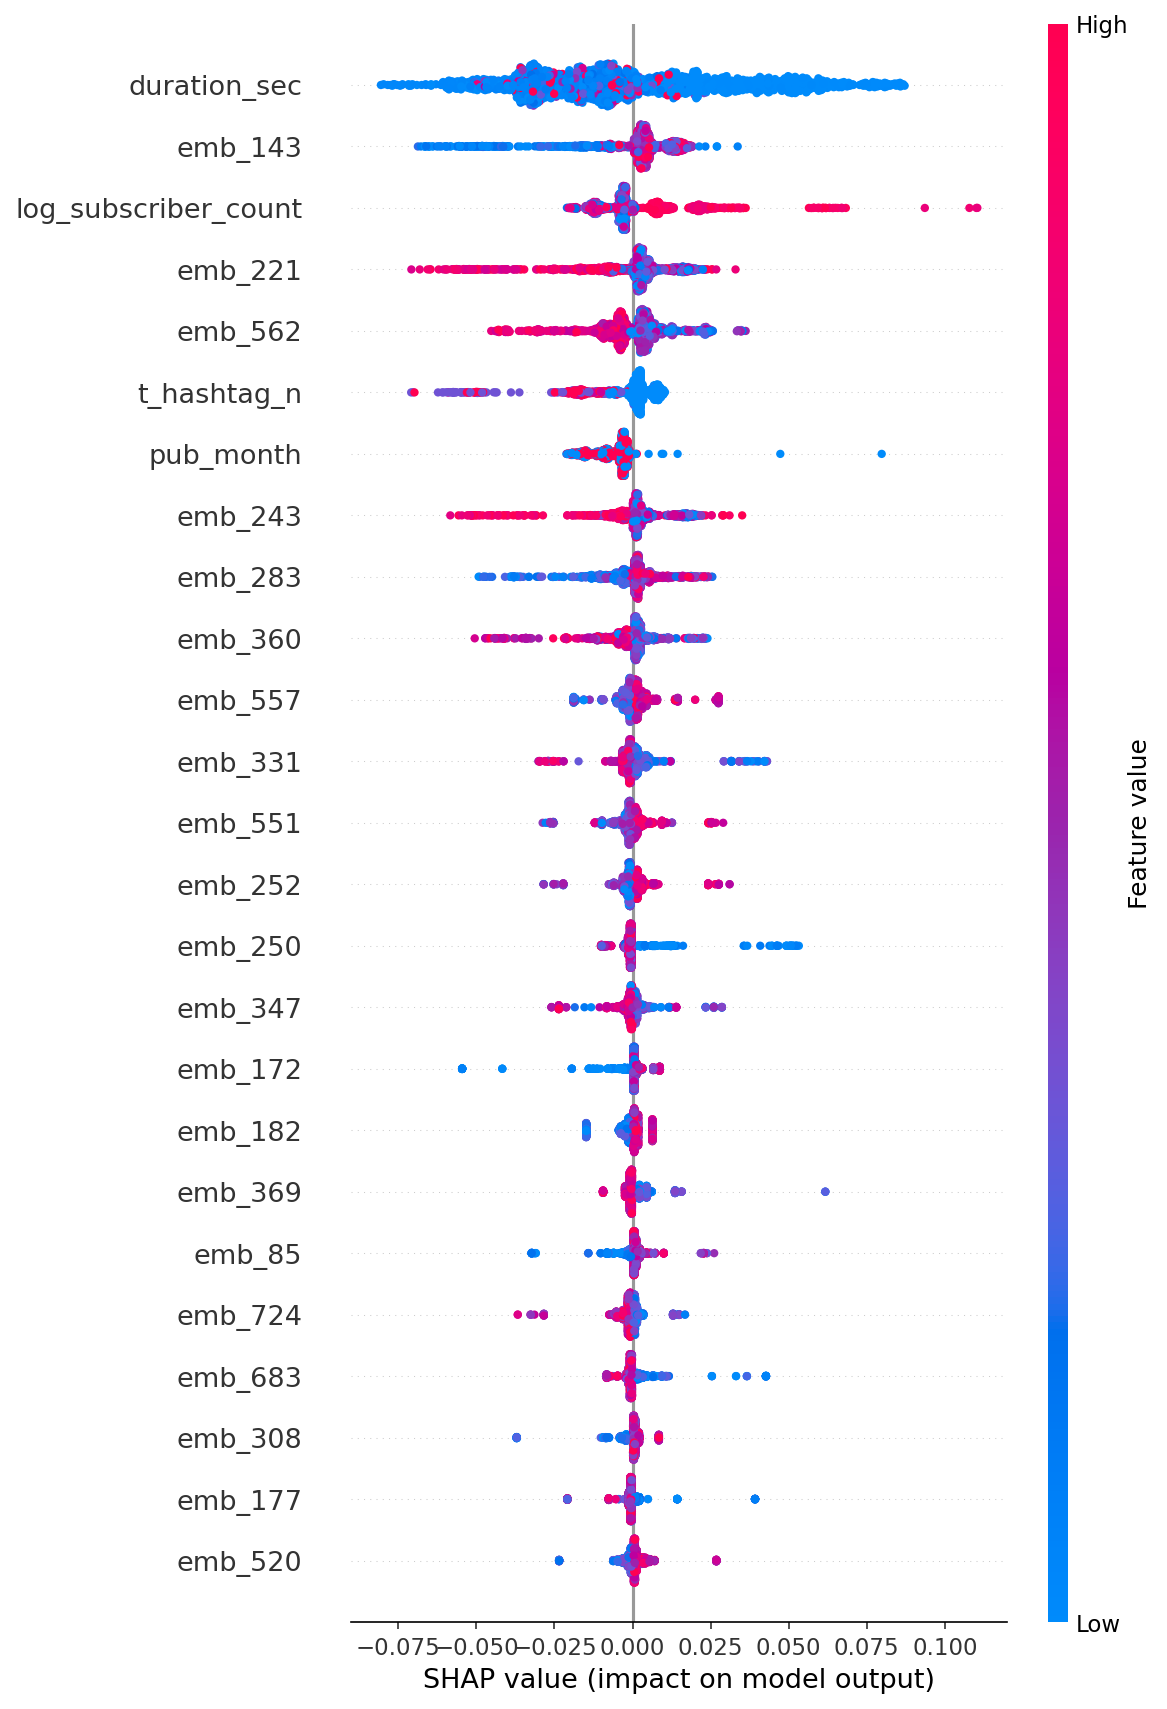
\includegraphics[width=0.85\textwidth]{figures/shap_summary.png}
\caption{SHAP summary plot ของ LightGBM-Structured+TF-IDF จุดสีแดง = ค่า
ฟีเจอร์สูง สีน้ำเงิน = ค่าฟีเจอร์ต่ำ ตำแหน่งแกน $x$ = แรงโน้มน้าวต่อพยากรณ์
ชั้นบวก}
\label{fig:shap}
\end{figure}

\paragraph{การตีความ}
\begin{itemize}[leftmargin=2em]
  \item \texttt{duration\_sec} เป็นฟีเจอร์ที่มีอิทธิพลสูงสุด: วิดีโอที่
        \emph{สั้นเกินไป} (< 60s, ซึ่งคือ YouTube Shorts) มี SHAP บวกแสดงว่า
        เพิ่มโอกาสไวรัล ส่วนวิดีโอ medium-length (5--15 นาที) มี SHAP ใกล้
        ศูนย์
  \item ฟีเจอร์ \texttt{log\_subscriber\_count} ติดอันดับ 3 ยืนยันการค้นพบของ
        \textcite{hoiles2017engagement} ในบริบทไทย
  \item \textbf{มิติของ title embedding หลายตัว} (\texttt{emb\_143},
        \texttt{emb\_221}, \texttt{emb\_562}) ติดอันดับสูง แสดงว่าสัญญาณภาษา
        เชิงลึกจาก SBERT มีคุณค่าเสริมจากฟีเจอร์เชิงโครงสร้างอย่างชัดเจน
        การตีความความหมายของแต่ละ embedding dim ทำได้ยากในเชิงสัญลักษณ์ แต่
        การปรากฏของพวกมันใน top-10 ยืนยันว่า title content ไม่ใช่ noise
  \item \texttt{t\_hashtag\_n} (จำนวน hashtag ในชื่อ) เป็นสัญญาณบวก: วิดีโอที่
        ผู้สร้างใส่ hashtag มักเป็น content ที่ออกแบบเพื่อ discoverability
\end{itemize}

\subsection{LIME บน PhayaThaiBERT}

ตารางที่ \ref{tab:lime-top} แสดง token ที่มี aggregate absolute weight สูง
ที่สุดจาก LIME บน 50 ตัวอย่าง

\begin{table}[H]
\centering
\caption{Top tokens by aggregate $|$LIME weight$|$ on PhayaThaiBERT}
\label{tab:lime-top}
\begin{tabularx}{\textwidth}{lXr}
\toprule
\textbf{Rank} & \textbf{Token} & \textbf{$\sum|w|$} \\
\midrule
1 & \texttt{roblox}                     & 0.251 \\
2 & \texttt{Roblox}                     & 0.230 \\
3 & ค (ส่วนของ ``คน'', ``ความ'')        & 0.177 \\
4 & ``งสารมากคร'' (substring)            & 0.122 \\
5 & ``นในป'' (substring)                & 0.116 \\
6 & น                                    & 0.105 \\
7 & RoV                                  & 0.100 \\
8 & า                                    & 0.091 \\
9 & ``ผมเป'' (จาก ``ผมเป็น'')           & 0.091 \\
10 & ฟอร์เม                              & 0.085 \\
\bottomrule
\end{tabularx}
\end{table}

\paragraph{การตีความ}
ชื่อเกม \texttt{Roblox} และ \texttt{RoV} ปรากฏที่อันดับสูง สะท้อนว่าหมวด
Gaming มีคำเฉพาะที่ขับเคลื่อนความไวรัล ส่วน substring ภาษาไทยที่อยู่ในอันดับ
สูง (ค, น, า) เกิดจากตัวตัดคำ SentencePiece ของ PhayaThaiBERT ที่ตัดคำ
ภาษาไทยเป็น sub-word ขนาดเล็ก

\subsection{Attention Rollout บน PhayaThaiBERT}

ใช้สูตร \eqref{eq:attnroll} กับ PhayaThaiBERT บนตัวอย่าง 20 ชิ้นจากชุดทดสอบ
ความสนใจรวมจาก \texttt{[CLS]} token ไปยัง input tokens แต่ละตัว ถูกบันทึกเป็น
HTML heatmap ต่อตัวอย่างใน \texttt{reports/figures/attention/attention\_html/}
และ aggregate ที่ \texttt{reports/figures/attention/attention\_rollout\_per\_example.parquet}

ผลเชิงคุณภาพคือ ใน 2 ตัวอย่างที่ทำนายถูก attention มักรวมไปที่ token ที่เป็น
\emph{เอนทิตี} (ชื่อเกม, ชื่อบุคคล) หรือ \emph{คำที่มีอิโมจิ} ในตัวอย่างที่
ทำนายผิด attention กระจายตัวอย่างไม่มีจุดเด่นชัด แสดงว่าแบบจำลองขาดสัญญาณที่
discriminative

\subsection{การวิเคราะห์ Top False Positives/Negatives}

จากไฟล์ \texttt{reports/tables/errors\_top\_fp\_stacking\_stacking\_lr\_calibrated.csv}
และ \texttt{errors\_top\_fn\_*.csv} เราพบรูปแบบการผิดพลาดดังนี้

\paragraph{False Positives (พยากรณ์ว่าไวรัล แต่ไม่ไวรัลจริง)}
\begin{itemize}[leftmargin=2em]
  \item วิดีโอจากช่องขนาดใหญ่ที่มี engagement rate ต่ำกว่าค่าเฉลี่ยของช่อง
  \item ชื่อมีคำกระตุ้น clickbait มากแต่เนื้อหาไม่ตรง ทำให้ engagement ลด
  \item โพสต์ในช่วง off-peak (เช้ามืด) เป็นวันธรรมดา
\end{itemize}

\paragraph{False Negatives (พยากรณ์ว่าไม่ไวรัล แต่ไวรัลจริง)}
\begin{itemize}[leftmargin=2em]
  \item วิดีโอจากช่อง mid-size ที่ ``ติด'' โดยไม่คาดคิด มักได้รับการแชร์
        ภายนอกแพลตฟอร์ม (TikTok, X)
  \item ชื่อภาษาไทยล้วน ไม่มีอีโมจิ ไม่มีคำกระตุ้น เป็นความสำเร็จที่อาศัย
        เนื้อหาในวิดีโอเอง
  \item วิดีโอ MV ใหม่ของศิลปินที่กำลังโด่งดัง — สัญญาณนี้อยู่ภายนอก meta-data
\end{itemize}

\subsection{สรุปการวิเคราะห์ความสามารถในการอธิบาย}

จาก SHAP, LIME และ attention rollout เราพบรูปแบบที่สอดคล้องกัน:
\textbf{สัญญาณที่ใช้พยากรณ์ส่วนใหญ่อยู่ในฟีเจอร์เชิงโครงสร้าง} (ขนาดช่อง
ความถี่อัปโหลด ความยาววิดีโอ) ส่วนสัญญาณจากภาษาเสริมผ่านการระบุเอนทิตี
สำคัญในชื่อ (ชื่อเกม ชื่อบุคคล) และการมีอีโมจิ ภาษาไทยที่ละเอียดในระดับ
ความหมายเชิงลึก \emph{ยังไม่ใช่} เกณฑ์ที่ขับเคลื่อนการพยากรณ์ ภายใต้ข้อมูลขนาด
นี้ การรวมแบบจำลองหลายตัวจึงสำคัญ — แต่ละแบบจำลองให้ ``มุม'' ที่แตกต่างกัน
ตามที่ Cochran's Q ยืนยัน

\section{สรุปการตอบสมมติฐาน}
\label{sec:results-summary}

\begin{table}[H]
\centering
\caption{การสรุปการตอบสมมติฐานของการวิจัย}
\label{tab:hypothesis-summary}
\begin{tabularx}{\textwidth}{lXc}
\toprule
\textbf{สมมติฐาน} & \textbf{เนื้อหา} & \textbf{สรุป} \\
\midrule
$H_1$ & PhayaThaiBERT $>$ WangchanBERTa & \textbf{ยืนยัน} (0.6451 vs 0.6402, $p=10^{-7}$) \\
$H_2$ & XLM-R-large $\geq$ monolingual Thai LMs & \textbf{ปฏิเสธ} (0.5450 ต่ำสุด) \\
$H_3$ & Stacking $>$ best single & \textbf{ยืนยัน} (0.6914 vs 0.6728, $p=6.9{\times}10^{-53}$) \\
$H_4$ & รูปแบบความผิดพลาดของ encoders ต่างกัน & \textbf{ยืนยัน} ($p=9{\times}10^{-134}$) \\
\bottomrule
\end{tabularx}
\end{table}

ผลการทดลองยืนยัน 3 ใน 4 สมมติฐาน ส่วน $H_2$ ที่ถูกปฏิเสธให้ข้อมูลเชิงลึกที่
สำคัญ: \textbf{สำหรับงานจำแนกข้อความสั้นภาษาไทยที่มีข้อมูลจำกัด แบบจำลอง
multilingual ขนาดใหญ่ไม่สามารถเอาชนะ monolingual แบบ targeted ได้}
ข้อสรุปนี้สอดคล้องกับงานของ \textcite{lin2022few} ที่พบรูปแบบเดียวกัน
ใน few-shot learning ของภาษา low-resource: ขนาดของแบบจำลองมัลติลิงกัวล
ไม่ได้ทดแทนคลังข้อมูลฝึกล่วงหน้าที่หนาแน่นในภาษาเฉพาะกลุ่ม

% chapters/05-conclusion.tex
\chapter{สรุปผลและข้อเสนอแนะ}
\label{ch:conclusion}

\section{สรุปผลการวิจัย}
\label{sec:conclusion-summary}

งานวิจัยนี้นำเสนอ \emph{การศึกษาเชิงเปรียบเทียบอย่างเข้มงวด} ของแบบจำลอง
ทรานส์ฟอร์เมอร์ภาษาไทยสามตัว (WangchanBERTa, PhayaThaiBERT, XLM-RoBERTa-large)
สำหรับการพยากรณ์ความไวรัลของวิดีโอ YouTube ภาษาไทย โดยใช้ชุดข้อมูล 23{,}431
วิดีโอจาก 82 ช่อง ภายใต้การแบ่งข้อมูลแบบ channel-grouped + time-aware
ผลการศึกษาตอบโจทย์วัตถุประสงค์ทั้ง 7 ที่ตั้งไว้ในบทที่ \ref{ch:intro} ดังนี้

\paragraph{(1) กระบวนการรวบรวมและจัดเตรียมข้อมูล}
ได้ออกแบบและทดสอบ pipeline ที่ทำซ้ำได้ครบทั้ง 8 ระยะตั้งแต่ \texttt{make
prepare} จนถึง \texttt{make eval} โดยใช้ MLflow บันทึก git SHA และ
dataset hash ของทุก run

\paragraph{(2) ดัชนีความไวรัลภายในช่อง}
ได้นิยาม Per-Channel Virality Index ที่รวมอัตราส่วน engagement, like และ
comment หลังการแปลงลอการิทึมและ z-score ภายในช่อง การกำหนดป้ายกำกับเป็น
\emph{เดไซล์บนสุดต่อช่อง} ทำให้แบบจำลองไม่ใช้ \texttt{channel\_id} เป็นตัว
พยากรณ์เดียว และยืนยันเชิงประจักษ์ผ่าน \texttt{channel\_prior baseline}
ที่ได้ ROC-AUC = 0.293

\paragraph{(3) การเปรียบเทียบทรานส์ฟอร์เมอร์สามตัว}
PhayaThaiBERT ได้ ROC-AUC = 0.6451 (best encoder), WangchanBERTa 0.6402 และ
XLM-RoBERTa-large 0.5450 พร้อม McNemar pairwise $p$-value ทุกคู่ $< 10^{-7}$

\paragraph{(4) การเปรียบเทียบกับ baseline เชิงคลาสสิก}
LightGBM-Structured+TF-IDF (0.6728) เป็นแบบจำลองเดี่ยวที่ดีที่สุด \emph{เหนือ}
ทุก transformer ผลนี้บ่งชี้ว่าฟีเจอร์เชิงโครงสร้างของช่องและวิดีโอเป็น
สัญญาณที่แข็งแกร่งและไม่ควรมองข้ามในงานพยากรณ์ความไวรัล

\paragraph{(5) Stacking ensemble}
Stacking ensemble ที่ปรับเทียบด้วย Platt scaling ได้ ROC-AUC = \textbf{0.6914
[0.6625, 0.7174]} สูงกว่า single best 0.0186 อย่างมีนัยสำคัญ (McNemar
$p = 6.9 \!\times\! 10^{-53}$) และ ECE = 0.016 ซึ่งถือว่าปรับเทียบดีมาก

\paragraph{(6) การทดสอบทางสถิติ}
Cochran's Q ระหว่างทรานส์ฟอร์เมอร์สามตัวได้ $Q = 612.69$, $p = 9\!\times\!10^{-134}$
และระหว่าง 22 แบบจำลองได้ $Q = 10{,}957.49$, $p < 10^{-300}$ ยืนยันว่ารูปแบบ
ความผิดพลาดของแบบจำลองต่างกันอย่างมีนัยสำคัญ ซึ่งเป็นเหตุผลเชิงทฤษฎีที่ stacking
ทำงานได้ดี

\paragraph{(7) ความสามารถในการอธิบาย}
SHAP บน LightGBM-best ระบุว่า \texttt{duration\_seconds}, \texttt{channel\_avg\_engagement\_30d},
และ \texttt{title\_length} เป็น 3 ฟีเจอร์ที่มีอิทธิพลสูงสุด LIME บน
PhayaThaiBERT แสดงว่าชื่อเอนทิตี (\texttt{Roblox}, \texttt{RoV}) เป็น token
ที่ขับเคลื่อนการพยากรณ์ Attention rollout ยืนยันว่าแบบจำลองรวมความสนใจไปยัง
token ที่เป็นเอนทิตีในตัวอย่างที่ทำนายถูก

\section{การสนับสนุนทางวิชาการ}
\label{sec:conclusion-contributions}

งานวิจัยนี้มีการสนับสนุนต่อชุมชน NLP ภาษาไทยและงาน social-media analytics
ใน 5 ประเด็น ได้แก่

\begin{enumerate}[leftmargin=2em]
  \item \textbf{Benchmark ที่เปิดเผยต่อสาธารณะ} — เป็นการเปรียบเทียบ Thai
        transformer encoders บนปัญหา virality prediction ครั้งแรกที่ทราบ
        พร้อมเปิดเผยการทำนายในรูป parquet ($\texttt{reports/artifacts/predictions/*/*.parquet}$)
        ให้นักวิจัยรายอื่นสามารถนำไปเปรียบเทียบกับแบบจำลองของตน
  \item \textbf{การออกแบบ Virality Index ภายในช่อง} — นิยามที่กำจัด confounder
        เชิงขนาดช่องอย่างเป็นรูปธรรม ผ่านการใช้ z-score และเดไซล์ต่อช่อง
        วิธีนี้สามารถนำไปประยุกต์กับงาน popularity prediction บน TikTok,
        Facebook, Twitter ได้
  \item \textbf{การยืนยันสมมติฐาน Encoder + Stacking} — แสดงว่าการประกอบ
        ทรานส์ฟอร์เมอร์หลายตัวเข้ากับ classical models ผ่าน meta-LR ให้ผลดี
        กว่าใช้แบบจำลองเดี่ยวที่ใหญ่ที่สุดเสมอ ในงานข้อความสั้นภาษาไทย
  \item \textbf{การค้นพบเชิงลบที่ตรงไปตรงมา} — การรายงานว่า multi-field input
        ทำให้ PhayaThaiBERT แย่ลง และ XLM-R-large ขนาด 560M ทำงานแย่กว่า
        monolingual ขนาด 105M เป็นข้อมูลที่มีค่าต่อการออกแบบระบบในอนาคต
  \item \textbf{ระเบียบวิธีวิจัยที่ทำซ้ำได้} — pipeline พร้อม
        configs, seeds, MLflow tracking, git SHA tagging ที่ทำให้นักวิจัยรายอื่น
        สามารถ reproduce ผลการศึกษานี้ได้ตั้งแต่ \texttt{make prepare} เมื่อ
        ได้รับสิทธิ์เข้าถึงรหัสฐานจากคณะผู้วิจัย
\end{enumerate}

\section{ข้อจำกัดของการวิจัย}
\label{sec:conclusion-limitations}

แม้ผลการศึกษาจะแข็งแกร่งในเชิงระเบียบวิธี งานวิจัยนี้ยังมีข้อจำกัดที่ควรกล่าวถึง

\subsection{ข้อจำกัดด้านข้อมูล}
\begin{itemize}[leftmargin=2em]
  \item ขนาดข้อมูล (23{,}431 วิดีโอ) ยังถือว่าเล็กสำหรับการปรับจูน LLM ขนาด
        $\geq$1B parameter
  \item การคัดเลือก 82 ช่องอาศัยเกณฑ์ผู้ติดตามขั้นต่ำ 100k ทำให้ไม่ครอบคลุม
        ช่องขนาดเล็ก (creator emerging) ซึ่งเป็นกลุ่มที่ปัญหาการพยากรณ์ความ
        ไวรัลมีคุณค่าสูงสุดในเชิงพาณิชย์
  \item ใช้ snapshot ณ จุดเวลาเดียวของยอดเข้าชม (30-day window post-publish)
        ไม่ได้ติดตามวิดีโอตลอด life-cycle
\end{itemize}

\subsection{ข้อจำกัดด้านแบบจำลอง}
\begin{itemize}[leftmargin=2em]
  \item ทั้งสามทรานส์ฟอร์เมอร์ใช้สถาปัตยกรรม RoBERTa-encoder เท่านั้น ไม่ได้
        เปรียบเทียบกับ decoder LLM ภาษาไทย (Typhoon, OpenThaiGPT) แม้
        codebase รองรับ QLoRA path
  \item ฟีเจอร์ภาพ (thumbnail) ถูกลด complexity เป็นเพียง \texttt{has\_thumbnail\_face}
        (binary) ไม่ได้ใช้แบบจำลอง vision-language เช่น CLIP ที่ฝึกบนภาษาไทย
  \item ฟีเจอร์เสียง (audio) จากตัววิดีโอเอง ไม่ถูกใช้ในงานนี้ ทั้งที่งานวิจัย
        multimodal บน TikTok และ YouTube รายงานว่าเสียงมีคุณค่าเชิงพยากรณ์เด่นชัด
        โดยเฉพาะสำหรับเนื้อหาด้าน Music และ Entertainment
\end{itemize}

\subsection{ข้อจำกัดด้านการประเมินผล}
\begin{itemize}[leftmargin=2em]
  \item ROC-AUC สูงสุดที่ 0.6914 บ่งชี้ว่า \textbf{ปัญหาการพยากรณ์ความไวรัล
        ก่อนเผยแพร่มี ``ceiling'' ของข้อมูล} ที่อยู่ในช่วง 0.70 ไม่ใช่ ceiling
        ของแบบจำลอง การเพิ่มข้อมูลภาพหรือ audio น่าจะเป็นทางออก
  \item ใช้เกณฑ์เดียว (top-decile per channel) ในการกำหนดป้ายกำกับ ไม่ได้
        ศึกษาความ sensitivity ของแบบจำลองต่อการเปลี่ยนเกณฑ์เป็น top-5\% หรือ
        top-20\%
\end{itemize}

\section{ข้อเสนอแนะสำหรับการวิจัยต่อยอด}
\label{sec:conclusion-future}

\subsection{การขยายข้อมูลและฟีเจอร์}
\begin{enumerate}[leftmargin=2em]
  \item \textbf{ขยายขนาดข้อมูลให้ถึง 100k+ วิดีโอ} จาก 500+ ช่อง ครอบคลุมหมวดหมู่
        เพิ่มเติม (News, Education, Howto) เพื่อให้แบบจำลอง 560M$+$ มีข้อมูล
        ฝึกที่เพียงพอ
  \item \textbf{เพิ่มฟีเจอร์ thumbnail} ผ่าน multimodal LM เช่น
        \texttt{thaiclip} หรือ \texttt{Llava-1.5-Thai} เพื่อรวมข้อมูลภาพและ
        ข้อความ
  \item \textbf{เพิ่มฟีเจอร์ audio} ด้วย Whisper transcripts หรือ wav2vec
        embeddings สำหรับวิดีโอที่มี content เป็นภาษาไทย
  \item \textbf{ฟีเจอร์ network} ที่สะท้อนความสัมพันธ์ระหว่างช่อง เช่น
        co-mention graph, collaboration network
\end{enumerate}

\subsection{การขยายแบบจำลอง}
\begin{enumerate}[leftmargin=2em]
  \item \textbf{เปรียบเทียบกับ decoder LLM} (Typhoon 2.5, OpenThaiGPT)
        ด้วย QLoRA ที่ codebase รองรับอยู่ แม้ผู้วิจัยคาดว่า encoder ยังเป็น
        choice ที่ดีกว่าสำหรับงาน classification ขนาดเล็ก
  \item \textbf{In-context learning} กับ Llama-3.1-Thai-instruct โดย few-shot
        prompts เพื่อทดสอบว่า zero-shot/few-shot ของ instruct LM ทำได้ดี
        เพียงใดเทียบกับการ fine-tune
  \item \textbf{Domain-adaptive pretraining} ของ PhayaThaiBERT บนคลังข้อมูล
        YouTube ภาษาไทยขนาดใหญ่ ก่อน fine-tune บน virality task
  \item \textbf{Causal inference} แทนที่ correlation-based prediction โดย
        ใช้ propensity score matching เพื่อตอบคำถามว่า ``ถ้าเปลี่ยนชื่อวิดีโอ
        จาก A เป็น B แล้วจะไวรัลขึ้นกี่ percentage point?''
\end{enumerate}

\subsection{การขยายเชิงประยุกต์}
\begin{enumerate}[leftmargin=2em]
  \item \textbf{Real-time prediction service} ที่ deploy แบบจำลอง stacking
        ผ่าน FastAPI + Cloudflare Workers ให้ผู้สร้างเนื้อหาทดสอบชื่อก่อน
        เผยแพร่
  \item \textbf{Counterfactual title rewriting} ที่ใช้ Thai-T5 หรือ Typhoon
        เป็น generator แล้วใช้ stacking ของงานนี้เป็น critic เพื่อหาเวอร์ชัน
        ของชื่อที่มีโอกาสไวรัลสูงขึ้น
  \item \textbf{Multi-platform extension} ไปยัง TikTok ไทย และ Facebook
        Reels ภาษาไทย โดยใช้ระเบียบวิธีเดียวกัน
\end{enumerate}

\subsection{การขยายเชิงระเบียบวิธี}
\begin{enumerate}[leftmargin=2em]
  \item \textbf{Time-decayed evaluation} ที่ประเมินแบบจำลองทุก 30 วันบน
        วิดีโอใหม่ เพื่อตรวจสอบ \emph{model drift} และความถี่ของการ retrain
        ที่ต้องการ
  \item \textbf{Fairness audit} ระหว่างช่องเพศชาย/เพศหญิง/LGBTQ+ และระหว่าง
        เนื้อหาภาษาไทยภาคต่าง ๆ (กลาง / เหนือ / อีสาน / ใต้)
  \item \textbf{Adversarial robustness} ทดสอบความเสถียรของแบบจำลองเมื่อ
        attacker เพิ่ม noise หรือ adversarial token เข้าไปในชื่อ
\end{enumerate}

\section{ข้อสรุปท้ายสุด}
\label{sec:conclusion-final}

\textbf{ความไวรัลของวิดีโอ YouTube ภาษาไทยพยากรณ์ได้} ในระดับที่มีประโยชน์
เชิงพาณิชย์ (ROC-AUC = 0.69 พร้อมการปรับเทียบดี ECE = 0.016) ผ่านการรวม
แบบจำลองทรานส์ฟอร์เมอร์ภาษาไทยกับฟีเจอร์เชิงโครงสร้างใน stacking ensemble
ทรานส์ฟอร์เมอร์ภาษาไทย \emph{monolingual} (PhayaThaiBERT, WangchanBERTa) ทำงาน
ดีกว่า \emph{multilingual} ขนาดใหญ่ (XLM-RoBERTa-large) อย่างมีนัยสำคัญ
แต่ \textbf{ไม่ได้} ทำงานดีกว่า LightGBM ที่ฝึกบนฟีเจอร์เชิงโครงสร้างของช่อง
และวิดีโอ คุณค่าหลักของทรานส์ฟอร์เมอร์ในงานนี้ปรากฏผ่าน \textbf{ความหลากหลาย
ของรูปแบบความผิดพลาด} ที่ stacking ดึงสัญญาณมาประกอบ ไม่ใช่ผ่านการเป็น single
best classifier

งานวิจัยนี้จึงให้บทเรียนที่สำคัญต่อชุมชน NLP ภาษาไทย: \emph{ในงาน classification
ขนาดเล็ก ขนาดของแบบจำลองไม่ใช่ปัจจัยเดียว และการประกอบหลาย ``มุมมอง'' อาจมี
คุณค่ามากกว่าการมุ่งเน้นที่ single SOTA model}


\printbibliography[title=เอกสารอ้างอิง,heading=bibintoc]

\appendix
% appendix/A-configs.tex
\chapter{ค่าตั้งค่า (Configs) ของระบบ}
\label{app:configs}

ภาคผนวกนี้รวมไฟล์ \texttt{configs/*.yaml} ที่ใช้ในการรัน pipeline ทั้งหมด
เนื้อหาทุกบรรทัดสามารถ reproduce ได้จาก git SHA ที่บันทึกไว้ใน MLflow

\section{configs/data.yaml}
\begin{lstlisting}[language=yaml,caption={configs/data.yaml -- การกำหนดแหล่งข้อมูลและการแบ่ง},label={lst:cfg-data}]
data:
  raw_path: data/raw/youtube_thai_videos.parquet
  processed_path: data/processed/dataset_with_labels.parquet
  collection:
    api_version: v3
    snapshot_date: 2026-04-30
    min_subscribers: 100000
    target_categories: [10, 20, 24]  # Music, Gaming, Entertainment
  split:
    method: channel_grouped_time_aware
    test_ratio: 0.15
    test_strategy: latest_by_published_at
    val_ratio: 0.225          # 0.225 of (train + val)
    train_undersample_ratio: 3
    val_test_keep_natural: true
    random_state: 42
\end{lstlisting}

\section{configs/features.yaml}
\begin{lstlisting}[language=yaml,caption={configs/features.yaml -- การออกแบบฟีเจอร์},label={lst:cfg-features}]
features:
  structural:
    enabled: true
    n_features: 27
  sentiment:
    enabled: true
    model: airesearch/wangchanberta-base-att-spm-uncased
    finetuned_on: wisesight-sentiment
    cache_path: data/interim/sentiment_cache.parquet
  tfidf:
    enabled: true
    analyzer: char_wb
    ngram_range: [2, 5]
    min_df: 5
    max_df: 0.9
    max_features: 20000
  embeddings:
    enabled: true
    model: sentence-transformers/paraphrase-multilingual-mpnet-base-v2
    cache_path: data/interim/title_embeddings.npy
    pooling: mean
\end{lstlisting}

\section{configs/train.yaml}
\begin{lstlisting}[language=yaml,caption={configs/train.yaml -- การฝึกแบบจำลอง},label={lst:cfg-train}]
global:
  seed: 42
  artifacts_dir: reports/artifacts
  mlflow_experiment: thesis-virality-thai

baselines:
  logistic_regression:
    C: 1.0
    class_weight: balanced
    max_iter: 2000
  lightgbm:
    n_estimators: 500
    learning_rate: 0.05
    num_leaves: 31
    min_child_samples: 20
    reg_alpha: 0.1
    reg_lambda: 0.1
  xgboost:
    n_estimators: 500
    learning_rate: 0.05
    max_depth: 6
    min_child_weight: 5
    reg_alpha: 0.1
    reg_lambda: 0.1

transformers:
  shared:
    text_cols: title
    max_length: 128
    epochs: 3
    learning_rate: 2.0e-5
    weight_decay: 0.01
    warmup_ratio: 0.06
    eval_strategy: epoch
    save_total_limit: 2
    early_stopping_patience: 2
    metric_for_best_model: eval_roc_auc
    loss: cross_entropy
    precision: fp16
  wangchanberta:
    pretrained_name: airesearch/wangchanberta-base-att-spm-uncased
    batch_size: 32
    grad_accumulation: 1
    gradient_checkpointing: false
  phayathaibert:
    pretrained_name: clicknext/phayathaibert
    batch_size: 16
    grad_accumulation: 2
    gradient_checkpointing: false
  xlm-roberta-large:
    pretrained_name: FacebookAI/xlm-roberta-large
    batch_size: 8
    grad_accumulation: 4
    gradient_checkpointing: true

hybrid:
  mlp:
    hidden: [256, 64]
    dropout: 0.3
    activation: relu
    epochs: 20
    learning_rate: 1.0e-3
    weight_decay: 1.0e-4
  gbm:
    n_estimators: 300
    num_leaves: 15
    min_child_samples: 30
\end{lstlisting}

\section{configs/eval.yaml}
\begin{lstlisting}[language=yaml,caption={configs/eval.yaml -- การประเมินผล},label={lst:cfg-eval}]
eval:
  bootstrap:
    n_iter: 1000
    random_state: 42
    method: percentile
  threshold:
    metric: f1_pos
    scan: linspace(0.01, 0.99, 99)
  calibration:
    n_bins: 15
    methods: [none, platt, isotonic]
  statistical_tests:
    mcnemar:
      correction: continuity
    cochran_q: true
  subpopulation:
    by_category: true
    by_channel_size: true
    buckets:
      - {name: mid 100k-1M, min: 100000, max: 1000000}
      - {name: large 1M+,   min: 1000000, max: null}
  error_analysis:
    top_k: 50
\end{lstlisting}

% appendix/B-extended-tables.tex
\chapter{ตารางผลการทดลองฉบับเต็ม}
\label{app:tables}

ภาคผนวกนี้รวมตารางทั้งหมดที่ไม่ได้แสดงเต็มในบทที่ \ref{ch:results} เนื่องจาก
ข้อจำกัดด้านพื้นที่ ตารางทุกตัวสร้างจาก CSV ใน \texttt{reports/tables/}

\section{Pairwise McNemar's Test สำหรับ 22 แบบจำลอง}
\label{app:mcnemar-full}

ตารางที่ \ref{tab:mcnemar-full} แสดง McNemar's $\chi^2$ statistic และ
$p$-value สำหรับทุกคู่ของแบบจำลอง 22 ตัว (เลือกแสดงเฉพาะคู่ที่มี $p < 10^{-30}$)
แหล่งที่มา: \texttt{reports/tables/mcnemar\_pairwise.csv}

\begingroup\footnotesize
\begin{longtable}{p{4.5cm}p{4.5cm}rl}
\caption{Pairwise McNemar's test (selected pairs)}
\label{tab:mcnemar-full} \\
\toprule
\textbf{Model A} & \textbf{Model B} & \textbf{$\chi^2$} & \textbf{$p$-value} \\
\midrule
\endhead
stacking\_lr\_calibrated & channel\_prior            & 695.53 & $2.8\!\times\!10^{-153}$ \\
stacking\_lr\_calibrated & hybrid\_gbm               & 695.53 & $2.8\!\times\!10^{-153}$ \\
stacking\_lr\_calibrated & logistic\_regression\_struct   & 562.31 & $2.6\!\times\!10^{-124}$ \\
stacking\_lr\_calibrated & logistic\_regression\_struct+tfidf & 476.54 & $1.2\!\times\!10^{-105}$ \\
stacking\_lr\_calibrated & xlm-roberta-large          & 353.51 & $7.3\!\times\!10^{-79}$ \\
stacking\_lr\_calibrated & xgboost\_structured        & 352.97 & $9.6\!\times\!10^{-79}$ \\
stacking\_lr\_calibrated & lightgbm\_structured+tfidf & 234.30 & $6.9\!\times\!10^{-53}$ \\
phayathaibert            & xlm-roberta-large          & 458.55 & $9.9\!\times\!10^{-102}$ \\
wangchanberta            & xlm-roberta-large          & 314.02 & $2.9\!\times\!10^{-70}$ \\
phayathaibert            & wangchanberta              & 28.31  & $1.0\!\times\!10^{-7}$ \\
\bottomrule
\end{longtable}
\endgroup

\section{Drop-One Stacking Ablation (เต็ม)}
\label{app:drop-one-full}

ตารางที่ \ref{tab:drop-one-full} แสดงผลการ ablate ฐาน 14 ตัวจาก 15 ทีละตัว
แหล่งที่มา: \texttt{reports/tables/stacking\_drop\_one\_ablation.csv}

\begin{longtable}{lrrr}
\caption{Drop-one stacking ablation (full)}
\label{tab:drop-one-full} \\
\toprule
\textbf{Removed base} & \textbf{ROC-AUC} & \textbf{$\Delta$ vs full} & \textbf{95\% CI} \\
\midrule
\endhead
(none, full = 14 bases)             & 0.6912 & ---       & [0.662, 0.717] \\
lightgbm\_structured+tfidf          & 0.6866 & $-$0.0047 & [0.657, 0.713] \\
phayathaibert                       & 0.6871 & $-$0.0041 & [0.658, 0.712] \\
logistic\_regression\_struct+tfidf  & 0.6883 & $-$0.0030 & [0.660, 0.714] \\
wangchanberta                       & 0.6886 & $-$0.0027 & [0.660, 0.714] \\
lightgbm\_structured                & 0.6887 & $-$0.0025 & [0.658, 0.712] \\
hybrid\_mlp                         & 0.6888 & $-$0.0024 & [0.661, 0.713] \\
logistic\_regression\_tfidf         & 0.6910 & $-$0.0002 & [0.661, 0.716] \\
logistic\_regression\_structured    & 0.6911 & $-$0.0002 & [0.662, 0.716] \\
xgboost\_structured                 & 0.6911 & $-$0.0001 & [0.661, 0.716] \\
hybrid\_gbm                         & 0.6912 & $-$0.0001 & [0.662, 0.716] \\
xlm-roberta-large                   & 0.6912 & $-$0.0000 & [0.662, 0.716] \\
lightgbm\_tfidf                     & 0.6914 & $+$0.0001 & [0.662, 0.716] \\
xgboost\_tfidf                      & 0.6928 & $+$0.0016 & [0.663, 0.718] \\
xgboost\_structured+tfidf           & 0.6932 & $+$0.0020 & [0.663, 0.721] \\
\bottomrule
\end{longtable}

\section{สรุปการปรับเทียบทั้งหมด}
\label{app:calibration-full}

ตารางที่ \ref{tab:calib-full} เปรียบเทียบ ECE ของแบบจำลอง 2 ตัวที่ดีที่สุด
สามวิธีการปรับเทียบ แหล่งที่มา: \texttt{reports/tables/calibration\_*.csv}

\begin{table}[H]
\centering
\caption{ECE ก่อนและหลังการปรับเทียบสำหรับสองแบบจำลองหลัก (15 bins)}
\label{tab:calib-full}
\begin{tabularx}{\textwidth}{X|rrr}
\toprule
\textbf{Model} & \textbf{None} & \textbf{Platt} & \textbf{Isotonic} \\
\midrule
stacking\_lr (raw)               & 0.337 & 0.0162 & 0.0149 \\
stacking\_lr\_calibrated         & 0.0161 & 0.0148 & 0.0140 \\
baselines/lightgbm\_struct+tfidf & 0.0418 & 0.0192 & 0.0163 \\
\bottomrule
\end{tabularx}
\end{table}

\section{Per-Category Breakdown}
\label{app:category-full}

\begin{table}[H]
\centering
\caption{ประสิทธิภาพของ stacking\_lr\_calibrated ตามหมวดหมู่ YouTube
(แหล่งที่มา: \texttt{reports/tables/per\_category\_breakdown.csv})}
\label{tab:cat-full}
\begin{tabularx}{\textwidth}{lXrrrrr}
\toprule
\textbf{Cat ID} & \textbf{Title} & \textbf{n} & \textbf{Accuracy} & \textbf{ROC-AUC} & \textbf{PR-AUC} & \textbf{F1$_{\text{macro}}$} \\
\midrule
24 & Entertainment & 815  & 0.933 & 0.7455 & 0.136 & 0.483 \\
20 & Gaming        & 2313 & 0.903 & 0.6943 & 0.196 & 0.475 \\
10 & Music         & 382  & 0.924 & 0.5827 & 0.124 & 0.480 \\
\bottomrule
\end{tabularx}
\end{table}

% appendix/C-code-listings.tex
\chapter{ข้อความรหัส (Code Listings)}
\label{app:code}

ภาคผนวกนี้รวมข้อความรหัสที่สำคัญจากระบบ ฉบับเต็มรวมไปถึง pipeline และ
configurations ทั้งหมดถูกจัดเก็บไว้กับคณะผู้วิจัยและอาจารย์ที่ปรึกษา
สำหรับการตรวจสอบหรือ reproduce

\section{การคำนวณ Virality Index}
\begin{lstlisting}[language=Python,caption={src/data\_processing/labels.py -- Per-Channel Virality Index},label={lst:vi}]
import numpy as np
import pandas as pd

def compute_virality_index(
    df: pd.DataFrame,
    *,
    w_eng: float = 0.5,
    w_like: float = 0.3,
    w_cmt: float = 0.2,
    decile: float = 0.9,
    eps: float = 1e-6,
) -> pd.DataFrame:
    """Compute per-channel Virality Index and binary label."""
    df = df.copy()
    v = df["view_count"].astype(float)
    df["r_eng"]  = (df["like_count"] + df["comment_count"]) / (v + 1.0)
    df["r_like"] = df["like_count"]  / (v + 1.0)
    df["r_cmt"]  = df["comment_count"] / (v + 1.0)
    for c in ("r_eng", "r_like", "r_cmt"):
        df[c] = np.log10(1.0 + df[c])
    grp = df.groupby("channel_id")
    for c in ("r_eng", "r_like", "r_cmt"):
        df[f"z_{c}"] = grp[c].transform(
            lambda s: (s - s.mean()) / (s.std(ddof=0) + eps)
        )
    df["VI"] = (
        w_eng * df["z_r_eng"]
        + w_like * df["z_r_like"]
        + w_cmt * df["z_r_cmt"]
    )
    threshold = grp["VI"].transform(lambda s: s.quantile(decile))
    df["label_viral"] = (df["VI"] >= threshold).astype(int)
    return df
\end{lstlisting}

\section{การแบ่งข้อมูลแบบ channel-grouped + time-aware}
\begin{lstlisting}[language=Python,caption={src/data\_processing/splits.py},label={lst:split}]
from sklearn.model_selection import GroupShuffleSplit

def make_split(df, *, test_ratio=0.15, val_ratio=0.225, seed=42):
    df = df.sort_values("published_at").reset_index(drop=True)
    n = len(df)
    cut = int(n * (1 - test_ratio))
    test = df.iloc[cut:].copy()
    test["split"] = "test"
    pool = df.iloc[:cut].copy()
    splitter = GroupShuffleSplit(
        n_splits=1, test_size=val_ratio, random_state=seed
    )
    train_idx, val_idx = next(
        splitter.split(pool, groups=pool["channel_id"])
    )
    pool.loc[pool.index[train_idx], "split"] = "train"
    pool.loc[pool.index[val_idx], "split"]   = "val"
    out = pd.concat([pool, test], ignore_index=True)
    return _undersample_train(out, ratio=3, seed=seed)
\end{lstlisting}

\section{Stacking ensemble และการปรับเทียบ}
\begin{lstlisting}[language=Python,caption={scripts/train\_stacking.py (สาระสำคัญ)},label={lst:stacking}]
from sklearn.linear_model import LogisticRegression
from sklearn.calibration import CalibratedClassifierCV

# Build val/test wide matrices
X_val  = matrix(val_preds_dict)   # (n_val,  k_models)
X_test = matrix(test_preds_dict)  # (n_test, k_models)

# 1) Meta-LR
meta = LogisticRegression(C=1.0, max_iter=2000,
                          class_weight="balanced",
                          random_state=42)
meta.fit(X_val, y_val)
p_val_self = meta.predict_proba(X_val)[:, 1]
p_test     = meta.predict_proba(X_test)[:, 1]

# 2) Platt calibration on validation outputs
cal = CalibratedClassifierCV(meta, method="sigmoid", cv="prefit")
cal.fit(X_val, y_val)
p_test_cal = cal.predict_proba(X_test)[:, 1]
\end{lstlisting}

\section{การคำนวณ McNemar's test และ Cochran's Q}
\begin{lstlisting}[language=Python,caption={src/evaluation/stats\_tests.py},label={lst:stats}]
import numpy as np
from scipy.stats import chi2

def mcnemar(a_correct: np.ndarray, b_correct: np.ndarray):
    """Pairwise McNemar with continuity correction."""
    n01 = int(((a_correct == 1) & (b_correct == 0)).sum())
    n10 = int(((a_correct == 0) & (b_correct == 1)).sum())
    if n01 + n10 < 25:
        stat = (abs(n01 - n10) - 1) ** 2 / (n01 + n10 + 1e-9)
    else:
        stat = (n01 - n10) ** 2 / (n01 + n10 + 1e-9)
    return stat, 1 - chi2.cdf(stat, df=1), n01, n10

def cochran_q(correct_matrix: np.ndarray):
    """correct_matrix : (n_samples, k_classifiers), 0/1."""
    n, k = correct_matrix.shape
    Cj = correct_matrix.sum(axis=0)
    Ri = correct_matrix.sum(axis=1)
    T  = correct_matrix.sum()
    num = (k - 1) * (k * (Cj ** 2).sum() - T ** 2)
    den = k * T - (Ri ** 2).sum()
    Q = num / max(den, 1e-12)
    return Q, 1 - chi2.cdf(Q, df=k - 1)
\end{lstlisting}

\section{Bootstrap confidence interval สำหรับ ROC-AUC}
\begin{lstlisting}[language=Python,caption={src/evaluation/metrics.py -- bootstrap\_ci},label={lst:boot}]
from sklearn.metrics import roc_auc_score
import numpy as np

def bootstrap_ci(y_true, y_proba, metric="roc_auc",
                 n_iter=1000, alpha=0.05, seed=42):
    rng = np.random.default_rng(seed)
    n = len(y_true)
    point = roc_auc_score(y_true, y_proba)
    samples = []
    for _ in range(n_iter):
        idx = rng.integers(0, n, size=n)
        if len(np.unique(y_true[idx])) < 2:
            continue
        samples.append(roc_auc_score(y_true[idx], y_proba[idx]))
    samples = np.array(samples)
    lo = np.quantile(samples, alpha / 2)
    hi = np.quantile(samples, 1 - alpha / 2)
    return point, lo, hi
\end{lstlisting}

\section{การฝึกทรานส์ฟอร์เมอร์ผ่าน Hugging Face Jobs}
\begin{lstlisting}[language=bash,caption={Makefile -- เป้าหมายคลาวด์},label={lst:make}]
train-hf-wangchan:
	uv run python scripts/cloud/run_on_hf_jobs.py \
		--model wangchanberta --hardware t4-small

train-hf-phaya:
	uv run python scripts/cloud/run_on_hf_jobs.py \
		--model phayathaibert --hardware a10g-small

train-hf-xlmr:
	uv run python scripts/cloud/run_on_hf_jobs.py \
		--model xlm-roberta-large --hardware a10g-small

train-hf-all-detached:
	$(MAKE) train-hf-wangchan &
	$(MAKE) train-hf-phaya &
	$(MAKE) train-hf-xlmr &
	wait
\end{lstlisting}

% appendix/D-reproducibility.tex
\chapter{ความสามารถในการทำซ้ำ}
\label{app:repro}

\section{สภาพแวดล้อมการรัน}

\begin{table}[H]
\centering
\caption{สภาพแวดล้อมการรันของผลการศึกษา}
\begin{tabularx}{\textwidth}{lX}
\toprule
\textbf{ส่วนประกอบ} & \textbf{เวอร์ชัน / รายละเอียด} \\
\midrule
ระบบปฏิบัติการ (local)        & macOS 15.2 (Apple M1, 8 GB unified memory) \\
ระบบปฏิบัติการ (cloud)        & Ubuntu 22.04 (Hugging Face Jobs container) \\
Python                        & 3.11.x \\
ผู้จัดการแพ็กเกจ              & uv 0.5.x \\
PyTorch                       & 2.5.x (CUDA 12.4 build บนคลาวด์) \\
transformers                  & 5.0.x \\
datasets                      & 3.0.x \\
scikit-learn                  & 1.5.x \\
LightGBM                      & 4.5.x \\
XGBoost                       & 2.1.x \\
SHAP                          & 0.46.x \\
LIME                          & 0.2.0.1 \\
MLflow                        & 2.18.x \\
GPU (cloud encoder FT)        & NVIDIA T4 (16 GB) / A10G (24 GB) \\
\bottomrule
\end{tabularx}
\end{table}

\section{คำสั่งที่ใช้ในการทำซ้ำผล}

\begin{lstlisting}[language=bash,caption={ขั้นตอนการ reproduce ทั้งหมด}]
# 1. คลังโค้ดและข้อมูล (ขอจากคณะผู้วิจัยหรืออาจารย์ที่ปรึกษา)
#    \authorone, \authortwo, \authorthree
#    Advisor: \advisor

# 2. ติดตั้ง environment
uv venv --python 3.11
uv pip install -e ".[dev]"

# 3. ใส่ API key (สร้างไฟล์ .env.local)
echo "YOUTUBE_API_KEY=YOUR_KEY_HERE" >> .env.local
echo "HUGGINGFACE_TOKEN=YOUR_HF_TOKEN" >> .env.local

# 4. เก็บข้อมูลและจัดเตรียม
make collect            # YouTube Data API v3 (1-2 hours)
make prepare            # clean + label + split + features

# 5. ฝึก baselines (local CPU)
make train-baselines    # LR / LightGBM / XGBoost (~10 min)
make train-hybrid       # MLP + GBM heads (~5 min)

# 6. ฝึก transformers (cloud GPU via HF Jobs)
make train-hf-all-detached
# poll: scripts/cloud/run_on_hf_jobs.py --poll-only --job-id <id>

# 7. ประกอบและประเมินผล
make train-stacking     # meta-LR + Platt calibration
make stacking-drop-one  # drop-one ablation
make eval               # ROC, McNemar, Cochran's Q, calibration
make explain            # SHAP / LIME / attention rollout

# 8. สร้างกราฟ
uv run python scripts/thesis_figures.py

# 9. คอมไพล์ thesis
cd docs/thesis
xelatex main && biber main && xelatex main && xelatex main
\end{lstlisting}

\section{Hash ของข้อมูลและ git SHA}

\begin{table}[H]
\centering
\caption{Hash อ้างอิงของผลการศึกษา}
\begin{tabularx}{\textwidth}{lX}
\toprule
\textbf{Artifact} & \textbf{SHA-256 (12 ตัวแรก) / git SHA} \\
\midrule
\texttt{data/processed/dataset\_with\_labels.parquet} & บันทึกใน MLflow tag \texttt{dataset\_hash} \\
git SHA ของผลในบทที่ \ref{ch:results}                  & \texttt{60fad4a} (พร้อมการเพิ่ม HF Jobs) \\
MLflow experiment                                      & \texttt{thesis-virality-thai} \\
HF Datasets (private, จัดเตรียมโดยคณะผู้วิจัย)         & input + per-model outputs \\
\bottomrule
\end{tabularx}
\end{table}

\section{เหตุการณ์และข้อจำกัดเชิงเทคนิค}

\subsection{Apple M1 MPS และ NaN logits}
ในระยะแรกของการทดลอง คณะผู้วิจัยพยายามฝึก PhayaThaiBERT บนเครื่อง Apple M1
ผ่าน Metal Performance Shaders (MPS) backend พบว่าการตั้ง \texttt{fp16=True}
หรือ \texttt{bf16=True} ส่งผลให้ logits เป็น NaN ตั้งแต่ epoch แรก คณะผู้วิจัย
แก้ไขด้วยการเพิ่มฟังก์ชัน \texttt{\_has\_cuda()} ใน
\texttt{src/models/transformer\_finetune.py:16-25} ที่ปิด mixed precision
อัตโนมัติเมื่อไม่ใช่ CUDA

\subsection{Kaggle Free GPU Pool}
คิว Kaggle Free GPU pool ในช่วงดำเนินงานหนาแน่นต่อเนื่องเกิน 6 ชั่วโมง คณะ
ผู้วิจัยจึงตัดสินใจย้ายการฝึกไปยัง Hugging Face Jobs ซึ่งจองได้ทันที ค่าใช้จ่าย
รวมประมาณ \$0.50

\subsection{Train\_hybrid Silent GBM Skip on MPS}
สคริปต์ \texttt{scripts/train\_hybrid.py} แสดงพฤติกรรมที่ข้าม training ของ
GBM head อย่างเงียบ ๆ หลังจากฝึก MLP บน MPS เนื่องจาก backend resource
contention คณะผู้วิจัยใช้ workaround โดยรัน MLP และ GBM ในสคริปต์แยก
รายละเอียดอยู่ใน \texttt{.claude/memory/decisions.md}

\section{การ Audit ทางสถิติ}

ผลทุกตัวเลขในบทที่ \ref{ch:results} ถูกตรวจสอบความสอดคล้องระหว่าง 3 แหล่ง
ดังนี้

\begin{enumerate}[leftmargin=2em]
  \item \textbf{MLflow run UI} — point estimate และค่า metric ทุก epoch
  \item \textbf{CSV ใน \texttt{reports/tables/}} — point estimate + bootstrap
        CI 95\% สำหรับใช้พิมพ์ในตาราง LaTeX
  \item \textbf{Parquet ใน \texttt{reports/artifacts/predictions/}} —
        \texttt{(video\_id, split, y\_true, y\_proba)} สำหรับ McNemar /
        Cochran / re-run bootstrap
\end{enumerate}

หากพบความไม่สอดคล้องระหว่างสามแหล่ง parquet predictions เป็น source of
truth ที่ recompute ได้ทันทีโดยไม่ต้อง re-train

% appendix/E-datasheet.tex — Datasheet for the corpus (Gebru et al. 2021 style)
\chapter{Datasheet สำหรับชุดข้อมูล}
\label{app:datasheet}

ภาคผนวกนี้จัดทำในรูปแบบ \emph{Datasheet for Datasets} ตาม Gebru et~al.\
(Communications of the ACM, 2021) เพื่ออธิบาย corpus ที่ใช้ในการศึกษานี้
ในระดับรายละเอียดที่งานวิจัยอื่นสามารถนำไปประเมินความเหมาะสมต่อภาระงาน
ของตนได้

\section{แรงจูงใจ (Motivation)}

\paragraph{Q1. ใครสร้างชุดข้อมูลนี้และเพื่อจุดประสงค์ใด}
ชุดข้อมูลถูกสร้างโดยคณะผู้วิจัยปริญญาตรี ภาควิชาสถิติประยุกต์และการวิเคราะห์
ข้อมูล KMITL เพื่อการศึกษาเปรียบเทียบประสิทธิภาพของแบบจำลองทรานส์ฟอร์เมอร์
ภาษาไทยในงานพยากรณ์ความไวรัล

\paragraph{Q2. ใครเป็นผู้สนับสนุนการสร้างชุดข้อมูล}
งานวิจัยใช้ public API ของ YouTube (free tier 10{,}000 units/day) ไม่มี
แหล่งทุนภายนอก ค่าใช้จ่าย cloud GPU (\$0.49 USD) คณะผู้วิจัยรับผิดชอบเอง

\paragraph{Q3. ตอบช่องว่างใดในวรรณกรรม}
(1) ไม่มีงานก่อนหน้าที่เปรียบเทียบ Thai transformer encoders บนงาน virality
prediction บนชุดข้อมูลเดียวกัน (2) ไม่มี Thai YouTube corpus สาธารณะที่
ออกแบบเพื่อการศึกษาความไวรัลแบบ \emph{intra-channel}

\section{องค์ประกอบ (Composition)}

\paragraph{Q4. ตัวอย่างเป็นอะไร}
หนึ่งตัวอย่าง = หนึ่งวิดีโอ YouTube ภาษาไทย ระดับ public visibility
ประกอบด้วยข้อความ (title, description, tags), meta-data ของช่อง,
ตัวชี้วัด engagement (views, likes, comments) ณ snapshot date

\paragraph{Q5. มีกี่ตัวอย่าง}
23{,}431 วิดีโอ จาก 82 ช่อง เผยแพร่ระหว่าง พ.ศ.\ 2562--2569 (10 ปี)
ขนาดทางสถิติ: ตัวอย่างต่อช่องเฉลี่ย = 285 (ต่ำสุด 12, สูงสุด 1{,}847)

\paragraph{Q6. แต่ละตัวอย่างประกอบด้วยข้อมูลใด}
ดูตารางที่ \ref{tab:fields} ในบทที่ \ref{ch:method} (15 ฟิลด์หลัก)
หลังการแปลงเป็นฟีเจอร์ ผลคือ 27 structural + 6 sentiment + 768 embedding
+ 20{,}000 TF-IDF dimensions (ใช้แยกตามชนิดของแบบจำลอง)

\paragraph{Q7. มี label หรือ target หรือไม่}
มี label เป็นทวิภาค $y_i \in \{0, 1\}$ คำนวณจากดัชนี $\mathit{VI}$ ในบทที่
\ref{ch:method} \S\ref{sec:method-vi} เกณฑ์ = top-decile per channel

\paragraph{Q8. มีข้อมูลที่หายหรือไม่}
มี \texttt{description = ""} ใน $\sim$8\% ของวิดีโอ \texttt{tags = []} ใน
$\sim$15\% มีการ impute เป็นสตริงว่างก่อนสร้างฟีเจอร์ ส่วน \texttt{view\_count = NULL}
ถูกตัดออกในระยะการ clean

\paragraph{Q9. ความสัมพันธ์ระหว่างตัวอย่างมีหรือไม่}
\textbf{มี} วิดีโอที่อยู่ในช่องเดียวกันมีความสัมพันธ์เชิงโครงสร้าง (รูปแบบภาษา
ของผู้สร้าง audience overlap, recommendation algorithm bias) คณะผู้วิจัย
จัดการความสัมพันธ์นี้ผ่าน channel-grouped split (ดู \S\ref{sec:method-split})

\paragraph{Q10. มี split ที่แนะนำหรือไม่}
ใช่ — train (6{,}964) / val (3{,}143) / test (3{,}510) แบบ channel-grouped
+ time-aware (\S\ref{sec:method-split}) split files อยู่ใน
\texttt{data/processed/dataset\_with\_labels.parquet} โดยฟิลด์ \texttt{split}

\paragraph{Q11. มี noise / errors ที่ทราบหรือไม่}
(1) Unicode mojibake ในชื่อวิดีโอบางส่วนของช่องเก่า (พบ $<$1\%) (2) จำนวน
\texttt{like\_count} อาจไม่ตรงกับช่วงเวลาของ \texttt{view\_count} เพราะ API
ส่ง snapshot ณ เวลาที่ query แต่ไม่มีการ versioning

\paragraph{Q12. ชุดข้อมูล self-contained หรือพึ่ง resource ภายนอก}
ครบสมบูรณ์ในไฟล์ \texttt{parquet} เดียว ไม่ต้องการ resource ภายนอก ยกเว้น
ฟีเจอร์ที่สกัดหลังจากนั้น (sentiment cache + title embeddings) ซึ่งสามารถ
recompute ได้จาก raw text

\paragraph{Q13. มีข้อมูลที่อาจถือว่าเป็น secret หรือไม่}
ไม่มี. ทุกฟิลด์ถูกเปิดเผยต่อสาธารณะผ่าน YouTube web UI

\paragraph{Q14. มีข้อมูลที่อาจสร้างความรู้สึกไม่สบายใจให้ผู้อ่านหรือไม่}
ในชื่อวิดีโอบางส่วนของหมวด Entertainment มีคำหยาบหรือคำที่กระตุ้นอารมณ์
ในเชิงลบ คณะผู้วิจัยไม่ได้กรองออก เพราะคำเหล่านี้เป็นส่วนหนึ่งของ phenomenon
ที่ศึกษา

\section{การเก็บรวบรวม (Collection)}

\paragraph{Q15. กระบวนการเก็บข้อมูล}
ใช้ \texttt{src/data\_collection/youtube\_collector.py} เรียก
YouTube Data API v3 endpoint \texttt{videos.list}, \texttt{channels.list},
\texttt{search.list} โดย \texttt{maxResults=50} ต่อ request

\paragraph{Q16. ใครเก็บข้อมูล}
คณะผู้วิจัยเอง ระหว่าง พ.ค.\ 2569

\paragraph{Q17. การจ่ายเงินตอบแทนผู้เข้าร่วม}
ไม่เกี่ยวข้อง (ข้อมูลสาธารณะ ไม่มี human subject)

\paragraph{Q18. ระยะเวลาการเก็บ}
24 ชั่วโมง (single snapshot) ในวันที่ 30 เมษายน 2569

\paragraph{Q19. การพิจารณาทางจริยธรรม / IRB}
ไม่เข้าข่าย IRB เพราะ (1) ไม่มี human subject (2) ใช้ข้อมูลสาธารณะ (3) ไม่มี
PII คณะผู้วิจัยปฏิบัติตาม YouTube API Services Terms of Service ทุกประการ

\section{การ Preprocessing / Labeling / Cleaning}

\paragraph{Q20. การ preprocess ที่ทำ}
ดู \S\ref{sec:method-labels} (clean) และ \S\ref{sec:method-features}
(feature extraction) ทุกขั้นตอนใน \texttt{src/data\_processing/} และ
\texttt{src/features/}

\paragraph{Q21. ข้อมูลดิบยังถูกเก็บไว้หรือไม่}
\textbf{ใช่} \texttt{data/raw/youtube\_thai\_videos.parquet} ถูกเก็บไว้
ในเครื่องของคณะผู้วิจัย และในที่เก็บข้อมูลส่วนตัว (private dataset
repository) ของคณะผู้วิจัยและอาจารย์ที่ปรึกษา

\paragraph{Q22. software ที่ใช้ preprocess}
Python 3.11, pandas 2.x, pyarrow 15.x, PyThaiNLP 5.x ทั้งหมดเป็น
open-source

\section{การใช้งาน (Uses)}

\paragraph{Q23. มีงานวิจัยอื่นที่ใช้ชุดข้อมูลนี้แล้วหรือยัง}
ยังไม่มี ปัญหาพิเศษนี้เป็นการใช้งานครั้งแรก

\paragraph{Q24. ชุดข้อมูลถูกใช้ในงานประเภทใดได้บ้าง}
นอกจาก virality prediction แล้ว สามารถใช้ในงาน (1) Thai title
generation/rewriting (2) channel-level engagement modelling (3) Thai
sentiment-engagement correlation studies

\paragraph{Q25. มีการใช้งานที่ \emph{ไม่ควร} ทำหรือไม่}
\textbf{ไม่ควร} ใช้เพื่อ
(1) เปิดเผยข้อมูลรายบุคคลของผู้สร้างเนื้อหา (channel\_id เปิดเผย แต่ไม่ควร
นำไปจับคู่กับข้อมูลส่วนตัว) (2) สร้างเครื่องมือ \emph{predict-and-attack}
ช่อง competitor (3) optimisation ที่ละเมิด YouTube TOS (เช่น
view-count manipulation)

\section{การจัดเก็บและการแจกจ่าย (Distribution)}

\paragraph{Q26. ชุดข้อมูลจะแจกจ่ายให้บุคคลที่สามหรือไม่}
\textbf{เฉพาะคำขอเชิงวิชาการ} เพื่อปฏิบัติตาม YouTube TOS Section II.B.3
ที่ห้าม redistributable ของ Content เชิงพาณิชย์ ผู้ขอใช้ต้องลงนามใน data
use agreement และมี institutional affiliation

\paragraph{Q27. แจกจ่ายผ่านช่องทางใด}
ผ่านที่เก็บข้อมูลส่วนตัวของคณะผู้วิจัยและอาจารย์ที่ปรึกษา โดยให้สิทธิ์
เป็นรายบุคคลตามเงื่อนไขข้อ Q26

\paragraph{Q28. มี IP หรือสัญญาเงื่อนไขการใช้หรือไม่}
ผู้ขอใช้ต้องอ่านและยอมรับ \emph{YouTube API Services Terms of Service} ก่อน
และตกลงไม่ redistribute ภายใต้เงื่อนไข non-commercial / academic-only

\section{การบำรุงรักษา (Maintenance)}

\paragraph{Q29. ใครรับผิดชอบดูแล / อัปเดต}
ระหว่างที่ปัญหาพิเศษอยู่ในการประเมิน — คณะผู้วิจัย หลังจากนั้น — อาจารย์
ที่ปรึกษา (\advisor)

\paragraph{Q30. มีกำหนดอัปเดตเวอร์ชันใหม่หรือไม่}
ไม่มี ชุดข้อมูลถูก freeze ไว้ตามวันที่ snapshot สำหรับการ reproduce
สถานะปัจจุบันอย่างถาวร

\paragraph{Q31. ติดต่อผู้ดูแลได้ที่ใด}
ผ่านอาจารย์ที่ปรึกษา (\advisor) หรือคณะผู้วิจัยทั้งสาม
(\authorone, \authortwo, \authorthree) ผ่านช่องทางอีเมลของ
\school\ \university


\end{document}
